\makeatletter
\def\input@path{{etc/}{body/}}
\makeatother

\documentclass[ALICE,manyauthors]{cernphprep}
\usepackage{ALICE_CDS_cernphprep}

\begin{document}

\begin{titlepage}
% the dates below correspond to CERN approval
% please don't touch: EB chairs will take care
\PHyear{2021}   % required, will be obtained from CERN
\PHnumber{XXX}  % required, will be obtained from CERN
\PHdate{11 Aug} % required, will be obtained from CERN
%%%%%%%%%%%%%%%%%%%%%%%%%%%%%%%%%%%%%%%%%%%%%%%%%%%%%%%%%%%%%%%%%%%%%%%%%%%%%%%

\title{Production of \kzero, \lmb (\almb), \Xis and \Oms in jets and underlying events in \pp and \pPb collisions with ALICE}
\ShortTitle{Production of (multi-)strange particles in jets and UE in \pp and \pPb}

%%% Do not change the next lines
\Collaboration{ALICE Collaboration\thanks{See Appendix~\ref{app:collab} for the list of collaboration members}}
\ShortAuthor{ALICE Collaboration} % appears on right page headers, do not change

\begin{abstract}
%!TEX root = ../AliStrangeJets.tex

\begin{abstract}
\label{sec:Abs}

In this paper, we explore the connection between the baryon-to-meson ratio enhancement and jet production via the measurement of the $\pT$-differential spectrum of strange and multi-strange particles ($\kzero$, $\lmb$, $\Xis$ and $\Oms$) in pp collisions at \thirteen and \pPb collisions at \fivenn both inclusively and within energetic jets with ALICE at LHC.
Furthermore, the the $\pT$-differential spectrum of multi-strange particle($\Xis$ and $\Oms$) in jets and underlying evens are reported here for the first time.
The $\pT$ dependent baryon-to-meson yield ratio in hadronic and nuclear collisions is sensitive to the collective expansion of the system, the partonic recombination into hadrons, the jet fragmentation and hadronization.
In $2<\pT< 6$~\GeVc, this ratio for inclusive hadrons is significantly enhanced at high multiplicity in small collision systems, such as \pp and \pPb collisions, relative to that at lower multiplicity.
A significant enhancement on production ratio between strange ($\kzero$, $\lmb$ ($\almb$), $\Xis$ and $\Oms$) and non-strange ($\pip + \pim$, p + $\pbar$) hadrons is observed with increasing event multiplicity in \pp and \pPb collisions.
The result of this paper set new constraints on the particle production mechanisms in jets, and provide new insight into the understanding of the origin of flow-like correlations observed in small systems.


\end{abstract}
\end{abstract}
\end{titlepage}
%%%%%%%%%%%%%%%%%%%%%%%%%%%%%%%%%%%%%%%%%%%%%%%%%%%%%%%%%%%%%%%%%%%%%%%%%%%%%%%

\setcounter{page}{2} %please do not remove this line

%%%%%%%%%%%%%%%%%%%%%%%%%%%%%%%%
% begin main text
%%%%%%%%%%%%%%%%%%%%%%%%%%%%%%%%

\section{Introduction}%
\label{sec:Introduction}

High-energy heavy-ion (A--A) collisions are expected to create, under extreme conditions of temperature and density, a deconfined state in which the degrees of freedom are partonic rather than hadronic, the Quark-Gluon Plasma (QGP)~\cite{Rafelski:126179, Satz:2000bn, Shuryak:1983ni, Jacak:2012dx, Cleymans:1985wb, Bass:1998vz, BraunMunzinger:2007zz}.
The structure and dynamical behavior of the QGP arise at the microscopic level from the interactions between quarks and gluons described by Quantum Chromodynamics (QCD)~\cite{Laermann:2003cv, Gupta:2011wh, Bhattacharya:2014ara}.
The interpretation of the heavy-ion results depends crucially on understanding results from small collision systems such as proton-proton (\pp) or proton-nucleus (p-A).
In \pPb collisions, where hot-matter effects are not expected, it is essential to investigate cold nuclear initial- and final-state effect as the baseline for heavy-ion collisions~\cite{Salgado:2011wc, Eskola:2016oht}.
On the other hand, \pp collisions constitutes a baseline for the nuclear effects in both A--A and p--A collisions.
In \pp collisions, there are not expected any hot and cold nuclear initial- and final-state effects.
So it constitutes a baseline for the nuclear effects in both A--A and p-A collisions.

Several collective phenomena have been observed in high-multiplicity \pp and \pPb collisions that are reminiscent of the observation attributed to the creation of QGP in \PbPb collisions~\cite{Aad:2015gqa, Abelev:2012ola, ABELEV:2013wsa, Khachatryan:2015waa, Acharya:2019vdf, Abelev:2014uua, Adam:2015vsf}.
These include the long-range angular correlations on the near and away side of a trigger particle~\cite{Aad:2015gqa, Abelev:2012ola, ABELEV:2013wsa}, non-vanishing 2$^\mathrm{nd}$ order Fourier coefficients ($v_{2}$) in multi-particle cumulant studies~\cite{Acharya:2019vdf, Khachatryan:2015waa}, etc.
In particular, in \pp and \pPb collisions, the baryon-to-meson ratios p$/\pi$ and $\Lambda/\kzero$ manifest an enhancement at intermediate $\pT$ ($\sim 3$~\GeVc)~\cite{Acharya:2018orn, Khachatryan:2016yru, Abelev:2013xaa, ALICE:2017jyt} which is qualitatively similar to that observed in \PbPb collisions.
The evolution of strange to non-strange hadron ratio increases as a function of \dndeta from low multiplicity \pp collisions to high multiplicity \pPb collisions and reaches the values observed in \PbPb collisions~\cite{Abelev:2013haa, ALICE:2017jyt, Khachatryan:2016yru}.
On the other hand, several measurements show the absence of a robust nuclear effect on the jet production at mid-rapidity in small systems~\cite{ALICE:2017svf, Acharya:2019jyg, Acharya:2019tku, ALICE:2014dla, Abelev:2013fn, Acharya:2018eat, Acharya:2017okq, Adam:2015xea, Adam:2016jfp}.
To understand particle production mechanisms in small collision systems, the separation of particle produced in hard processes (jet) from those of the underlying event is important.
In a recent study, the ALICE Collaboration has studied baryon-to-meson ratios with a new method: by studying the ratios in two parts of the events separately -- inside jets and in the event portion perpendicular to a jet cone in \pp collisions at \seven and \pPb collisions at \fivenn~\cite{Acharya:2021oaa}.
It is shown that the $(\lmb + \almb)/2\kzero$ ratio at intermediate $\pT$ found in the inclusive particle measurements in \PbPb and high multiplicity small collision systems is not present for particles associated with hard scatterings tagged by jets.
In this contribution, the baryon-to-meson ratio and multi-strange-to-strange particle ratio will be studied in charged-particle jets and underlying event.
It will provide further insight into disentangling the soft process or hard scattering contributions of the baryon-to-meson ratio enhancement at intermediate $\pT$ and the strange particle production increasing with multiplicity in small systems.

In this paper, the production of \kzero, \lmb (\almb), \Xis and \Oms in charged-particle jets and underlying event in \pp collisions at \thirteen and \pPb collisions at \fivenn is reported.
Strange particles are reconstructed in the pseudo-rapidity range $|\eta| < 0.75$.
Jets are reconstructed in the transverse momentum range $\pTjch > 10$~\GeVc and in the pseudo-rapidity range $|\eta| < 0.35$.
The (multi-)strange particles associated with the jet are defined as a function of distance between particle momentum and jet axis in $\eta-\varphi$ plane.
The results presented in this paper significantly improve the precision of the $\pT$-differential measurements  compared to ALICE previous one~\cite{Acharya:2021oaa}, including also the centrality dependence and extending to the multi-strange sector in both pp (at different energy) and p–Pb collisions.
The baryon-to-meson and baryon-to-baryon ratios in energetic jets are compared with the case of particles not associated with jets and PYTHIA~8~\cite{Sjostrand:2014zea} simulation.

The paper is structured as follows.
In Sec.~\ref{sec:Detector}, the ALICE apparatus and the data samples used for the analysis are presented. In Sec.~\ref{sec:Analysis}, the methods adopted for charged-particle jet reconstruction, (multi-)strange particle reconstruction, and particle-jet matching are described.
Estimated of the associated systematic uncertainties are also reported in Sec.~\ref{sec:Analysis}.
The transverse momentum dependence of (multi-)strange hadrons distributions and particle ratios, the model comparisons, and an interpretation of the results are presented and discussed in Sec.~\ref{sec:Results}.

\section{ALICE detector and data selection}%
\label{sec:Detector}

A detailed description of the ALICE apparatus and its performance can be found in~\cite{Collaboration_2008, Abelev:2014ffa}.
This analysis relies on the central tracking system and the forward VZERO detector~\cite{Abbas:2013taa}.
The two forward scintillator arrays V0A (covering pseudo-rapidity range of $2.8 < \eta < 5.1$), and V0C ($-3.7 < \eta < -1.7$) were employed for both as triggering detectors and to determine the event multiplicity class.
The main central barrel detectors used for this analysis are the Inner Tracking System (ITS)~\cite{Aamodt:2010aa}, the Time Projection Chamber (TPC)~\cite{Alme:2010ke} and the Time Of Flight detector (TOF)~\cite{Akindinov:2004cj, Akindinov:2009zze, Akindinov:2010zzb, Carnesecchi:2018oss}, which cover the pseudo-rapidity region $|\eta| < 0.9$ and are located inside a large solenoidal magnet providing a 0.5~T magnetic field.

The innermost barrel detector is the ITS consisting of six cylindrical layers of high spatial resolution silicon detector using three different technologies.
The two innermost layers~(SPD) are based on silicon pixel technology and cover $|\eta| < 2.0$ and $|\eta| < 1.4$, respectively.
The SPD was used to reconstruct the collision's primary vertex and short track segments, which are called "tracklets".
The four outer ITS layers consist of silicon drift (SDD) and strip (SSD) detectors, with the outermost layer having a radius $r = 43$~cm.
The SDD and SSD are able to measure the specific ionization energy loss (\dEdx) with a relative resolution around $10\%$ in the low $\pT$ region (up to $\sim 1$~\GeVc).
The ITS is also used to reconstruct and identify low momentum particles down to $100$~\MeVc that can not reach the TPC.

The TPC is a large cylindrical drift detector which is filled with a $\mathrm{Ne-CO_{2}}$ gas mixture.
The radius and the longitude dimensions of the TPC are about $85 < r < 250 $~cm and $-250 < z < 250 $~cm, respectively.
As the main tracking device, the TPC provides full azimuthal acceptance for tracks in the pseudo-rapidity region $|\eta| < 0.9$.
In addition, it provides charged-hadron identification via measurement of the specific ionization energy loss \dEdx.
At low transverse momenta ($\pT \lesssim 1.0$~\GeVc), the \dEdx resolution of 5.2\% for a minimum ionizing particle allows a track-by-track identification. On the other hand, at high transverse momenta ($\pT \gtrsim 2.0$~\GeVc), the overlapping energy loss has to be statistically distinguished via a multi-Gaussian fit to the \dEdx distributions.

Outside of the TPC and located at a radius of approximately $4$~m, the TOF measures the particles' time of flight.
The TOF is a cylindrical array of multi-gap resistive plate chambers with an intrinsic time resolution of $50$~ps.
It covers the pseudo-rapidity range $\abs{\eta} < 0.9$ with full azimuthal acceptance.
It can provide particle identification over a broad range at intermediate transverse momenta ($0.5 \lesssim \pT \lesssim 2.7$~\GeVc).
The total time-of-flight resolution, including the collision time resolution, is about $90$~ps in \pp and \pPb collisions~\cite{Acharya:2020uxl, Jacazio:2018slq}.

Data of \pp collisions at \thirteen and of \pPb collisions at \fivenn are used in this analysis.
The \pp data sample was recorded in $2016$--$2017$, the \pPb sample in 2016 with ALICE detector, respectively.
The data were collected with a minimum bias (MB) trigger requiring at least one hit in both V0 scintillators in coincidence with proton bunches' arrival from both directions.
Interaction vertices are reconstructed by the extrapolation of ITS track segments towards the nominal interaction point.
Pile-up events, due to multiple interactions in the triggered bunch crossing, are removed by exploiting the correlation between the number of pixel hits and the number of SPD tracklets.
In addition, the coordinate of the primary vertex along the beam direction is within $\pm 10$~cm with respect to the ALICE nominal interaction point.
After event selection, the \pp sample consists of $1.5$ billion events.
The average number of inelastic interactions per bunch crossing ranges between $2\%$ and $14\%$.
The integrated luminosity of $\lumi_{\rm int} = 9.38\pm 0.47$~nb$^{-1}$ based on the visible cross section observed by the V0 trigger was extracted from a van der Meer scan~\cite{ALICE-PUBLIC-2016-002}.
About $500$ million events from the \pPb samples were selected, which correspond to an integrated luminosity of $\lumi_{\rm int} = 295 \pm 11 $~$\mu{\rm b}^{-1}$~\cite{ALICE:2019oyn}.
The \pPb events were divided into three multiplicity classes based on the total charge deposited in the V0A (the Pb-going direction).
The multiplicity intervals and their corresponding mean charged-particle density (\dndeta) measured at mid-rapidity ($\abs{\eta} < 0.5$) are given in Ref.~\cite{Adam:2015pza}.

\section{Analysis}%
\label{sec:Analysis}

\subsection{Charged-particle jet reconstruction}%
\label{sec:JetRec}

In this analysis, the FastJet package~\cite{Cacciari:2011ma} is used to find jets using charged particles with the \akT algorithm~\cite{Cacciari:2008gp}.
The \akT algorithm is a commonly used jet finding algorithm which starts particle clustering from the highest momentum particles, in contrast to the $\kT$ algorithm, which does the opposite.
Charged particles, which are used as input for jet reconstruction, are reconstructed using ITS and TPC information.
The charged particle tracks are selected in $\abs{\eta_{\rm trk}} < 0.9$ ($\TPC$ acceptance) and $\pT> 0.15$~\GeVc.
The jet resolution parameter is $R = 0.4$ and the reconstructed jet clusters are selected in $\abs{\eta_{\rm jet}} < 0.35$.
This condition ensures the jet cone is fully overlapping with the acceptances of both charged-particle tracks and the strange particles ($|\eta| < 0.75$).
A $\pTj^{\rm ch} > 10$~\GeVc cut on charged-particle jet transverse momentum, according to ALICE previous study~\cite{Acharya:2021oaa} is applied, to tag the hard scattering process.


Besides the hard parton-parton interactions in the collisions, there is also the soft contribution which did not correlate with the hard collisions.
The background density~($\rhobkg$) determined from the $\kT$ algorithm~\cite{Catani:1993hr, Ellis:1993tq} in \pp collisions is around $1$~\GeVc~rad$^{-1}$ and is not subtracted.
In \pPb collisions, the underlying background is larger and the reconstructed jet is therefore further corrected for contributions from the underlying event to the jet momentum as
\begin{equation}
\pTj = \pTjch - \rhobkg\cdot\Ajet
\label{eq:DeltaPt}
\end{equation}
where the $\pTj^{\rm rec}$ is the reconstructed jet $\pT$, $\Ajet$ is the jet area and $\rhobkg$ is the event-by-event background density~\cite{Cacciari:2007fd}.
The $\Ajet$ is calculated using the FastJet algorithm with a ghost area of $0.005$~\cite{Cacciari:2008gn}.
A method that is suitable for the background density estimation for sparse systems to circumvent the problems arising from using the ghost jets is introduced in \cite{Chatrchyan:2012tt}.
The basic idea is to neglect the ghosts and instead account for the empty areas by introducing a factor correcting the background density for it.
It can be implemented by the following formula
\begin{equation}
\rhobkg = C\cdot{\rm median}\{\frac{p_{\rm T,i}}{A_{i}}\} ~ {\rm with}~ C = \frac{\sum_{j}A_{j}}{A_{\rm acc}}.
\label{eq:RhoCMS}
\end{equation}
Where $A_{j}$ is the area of each $\kT$ jet with at least one real track, i.e. excluding ghosts and $A_{\rm acc}$ is the area of the charged-particle acceptance, namely $(2 \times 0.9) \times 2\pi$.
This method has the advantage that it uses the median and takes empty areas into account.
This method can be further refined for the specific case of \pPb collisions.
It can be shown that the exclusion of the two $\kT$ jets with highest $\pT$ from Eq.~(\ref{eq:RhoCMS}) is enhancing the background quality~\cite{ALICE:2015umm, ALICE:2016faw}.

\subsection{Strange particles reconstruction}%
\label{sec:ParRec}

The strange particles \kzero, \lmb, \almb, \Xis and \Oms are reconstructed at mid-rapidity ($\abs{\eta} < 0.75$) via their specific weak decay topology.
The following decay channels are studied~\cite{PhysRevD.98.030001}:
$$
\begin{aligned}
\kzero      & \to \pip + \pim               & B.R. & = (69.20 \pm 0.05) \%, \\
\lmb (\almb) & \to \mathrm{p}(\pbar) + \pim (\pip)    & B.R. & = (63.9  \pm 0.5)  \%, \\
\X (\Ix)    & \to \lmb (\almb) + \pim (\pip) & B.R. & = (99.887 \pm 0.035) \%, \\
\Om (\Mo)   & \to \lmb (\almb) + \kam (\kap) & B.R. & = (67.8  \pm 0.7)  \%. \\
\end{aligned}
$$
The proton, pion, and kaon tracks (daughter tracks) are identified in the TPC via their measured energy deposition~\cite{Abelev:2014ffa}.
The identification of the \Vzero (\kzero and \lmb (\almb) which decay into two oppositely charged daughter particles) and cascade (\Xis and \Oms which decay into a bachelor charged meson plus a \Vzero decaying particle, giving the cascade decay topology) candidates follows those presented in earlier ALICE publications~\cite{Aamodt:2011zza, Abelev:2012jp, Acharya:2018orn, Abelev:2013haa, Acharya:2020uxl, Acharya:2019kyh}.
In addition, removal of contributions from pileup collisions outside the trigger proton bunch (``out-of-bunch pileup''), it is achieved by requiring  that at least one of the charged decay track matches a hit in a ``fast'' detector (either the ITS or the TOF detector).
The selections used in this paper are summarized in Tab.~\ref{tab:V0Cut}, \ref{tab:CascadeCut}.

The signal extraction is performed as a function of $\pT$.
In each $\pT$ interval, an invariant mass histogram is filled with the corresponding counts.
Then a Gaussian function is used to fit the signal, and a linear function is used to fit the combinatorial background.
This allows for the extraction of the mean ($\mu$) and width ($\sigma$) of the signal.
A ``peak'' region is defined within $\pm 6\sigma$ for \Vzeros and $\pm 3\sigma$ ($\pm 4\sigma$) for cascades in \pp (and \pPb) with respect to $\mu$ for each $\pT$ bin.
The ``background'' regions are defined on both sides of the peak region.
The $\pT$-differential yields of (multi-)strange particles are obtained by subtraction the integral of the background fit function in the peak region from the total bin counting in the same region.
Examples of the invariant mass signal for all particles are shown in Fig.~\ref{fig:InvM}.
\begin{figure}[!ht]
\begin{center}
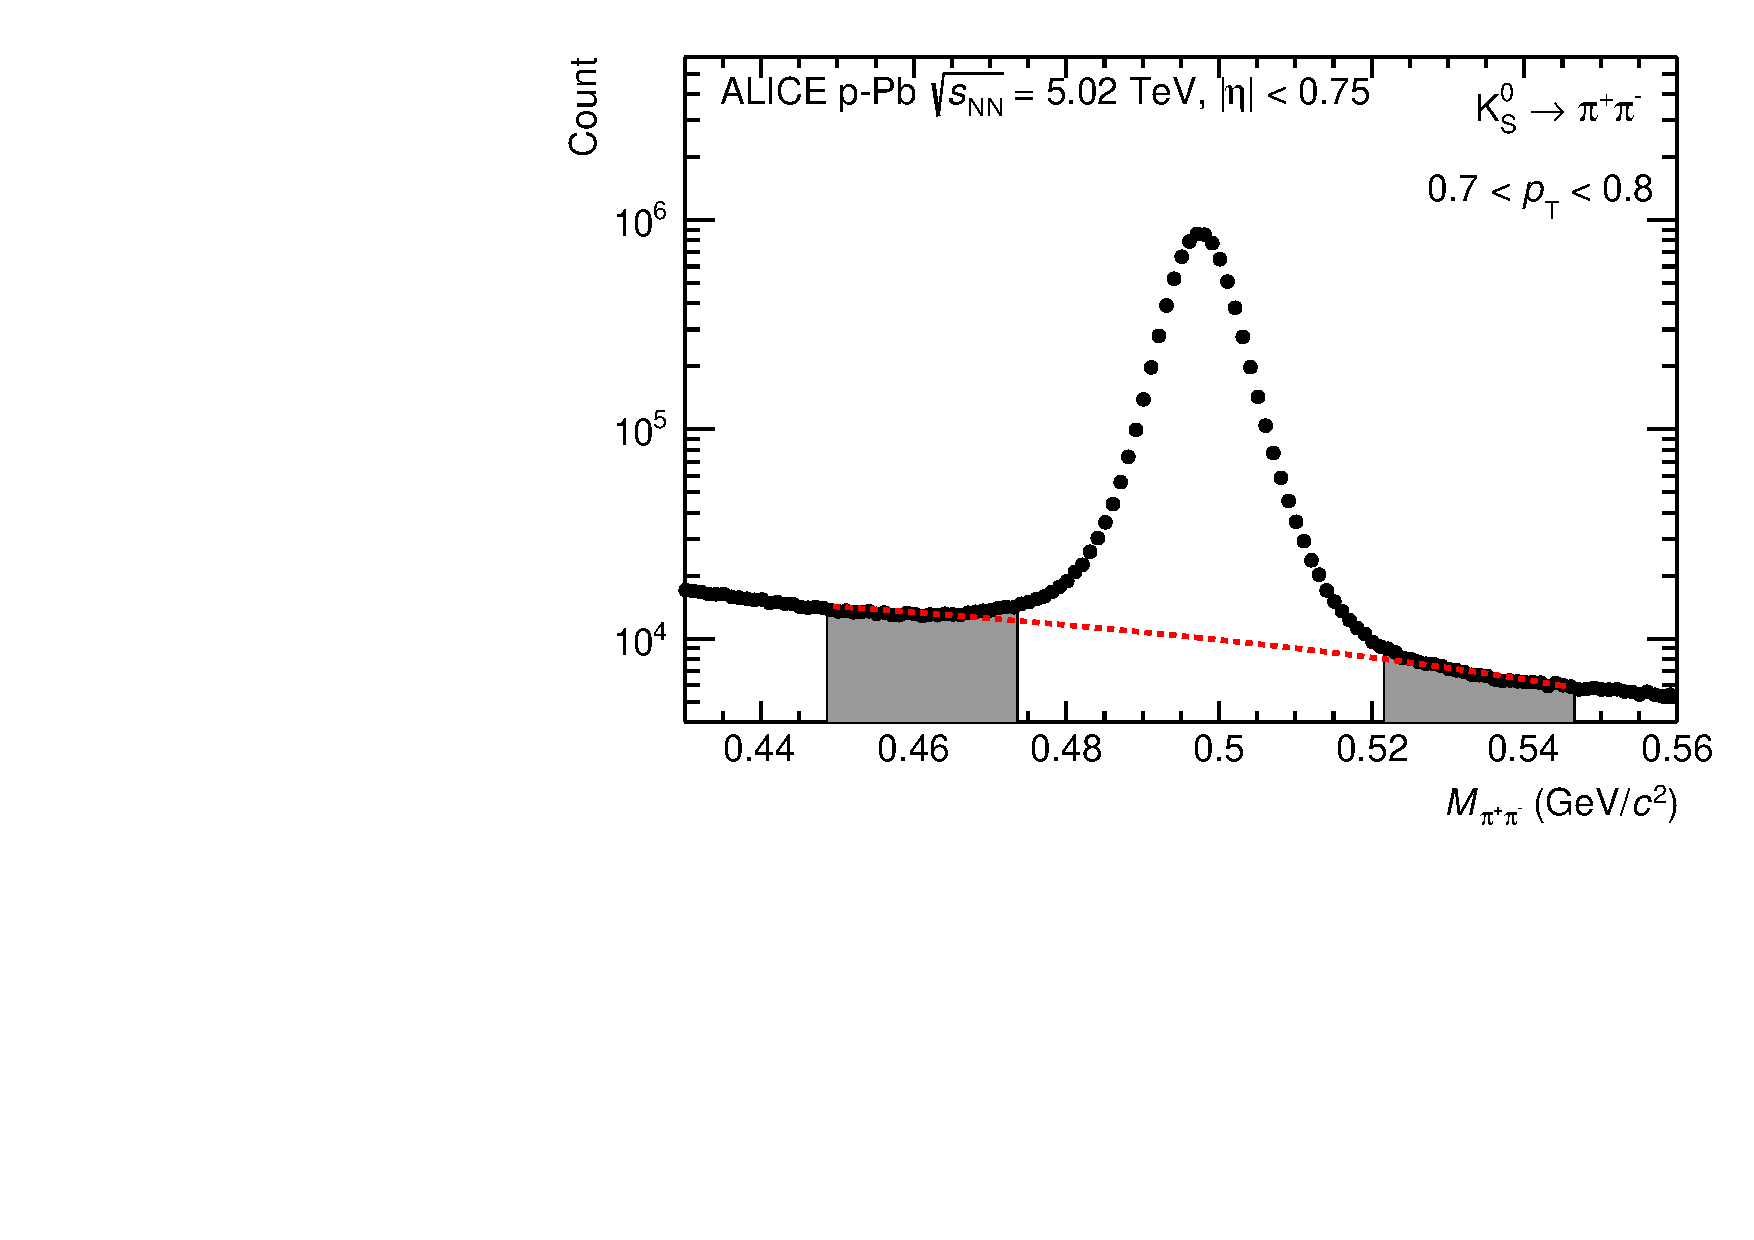
\includegraphics[width=.49\textwidth]{cf01_1}
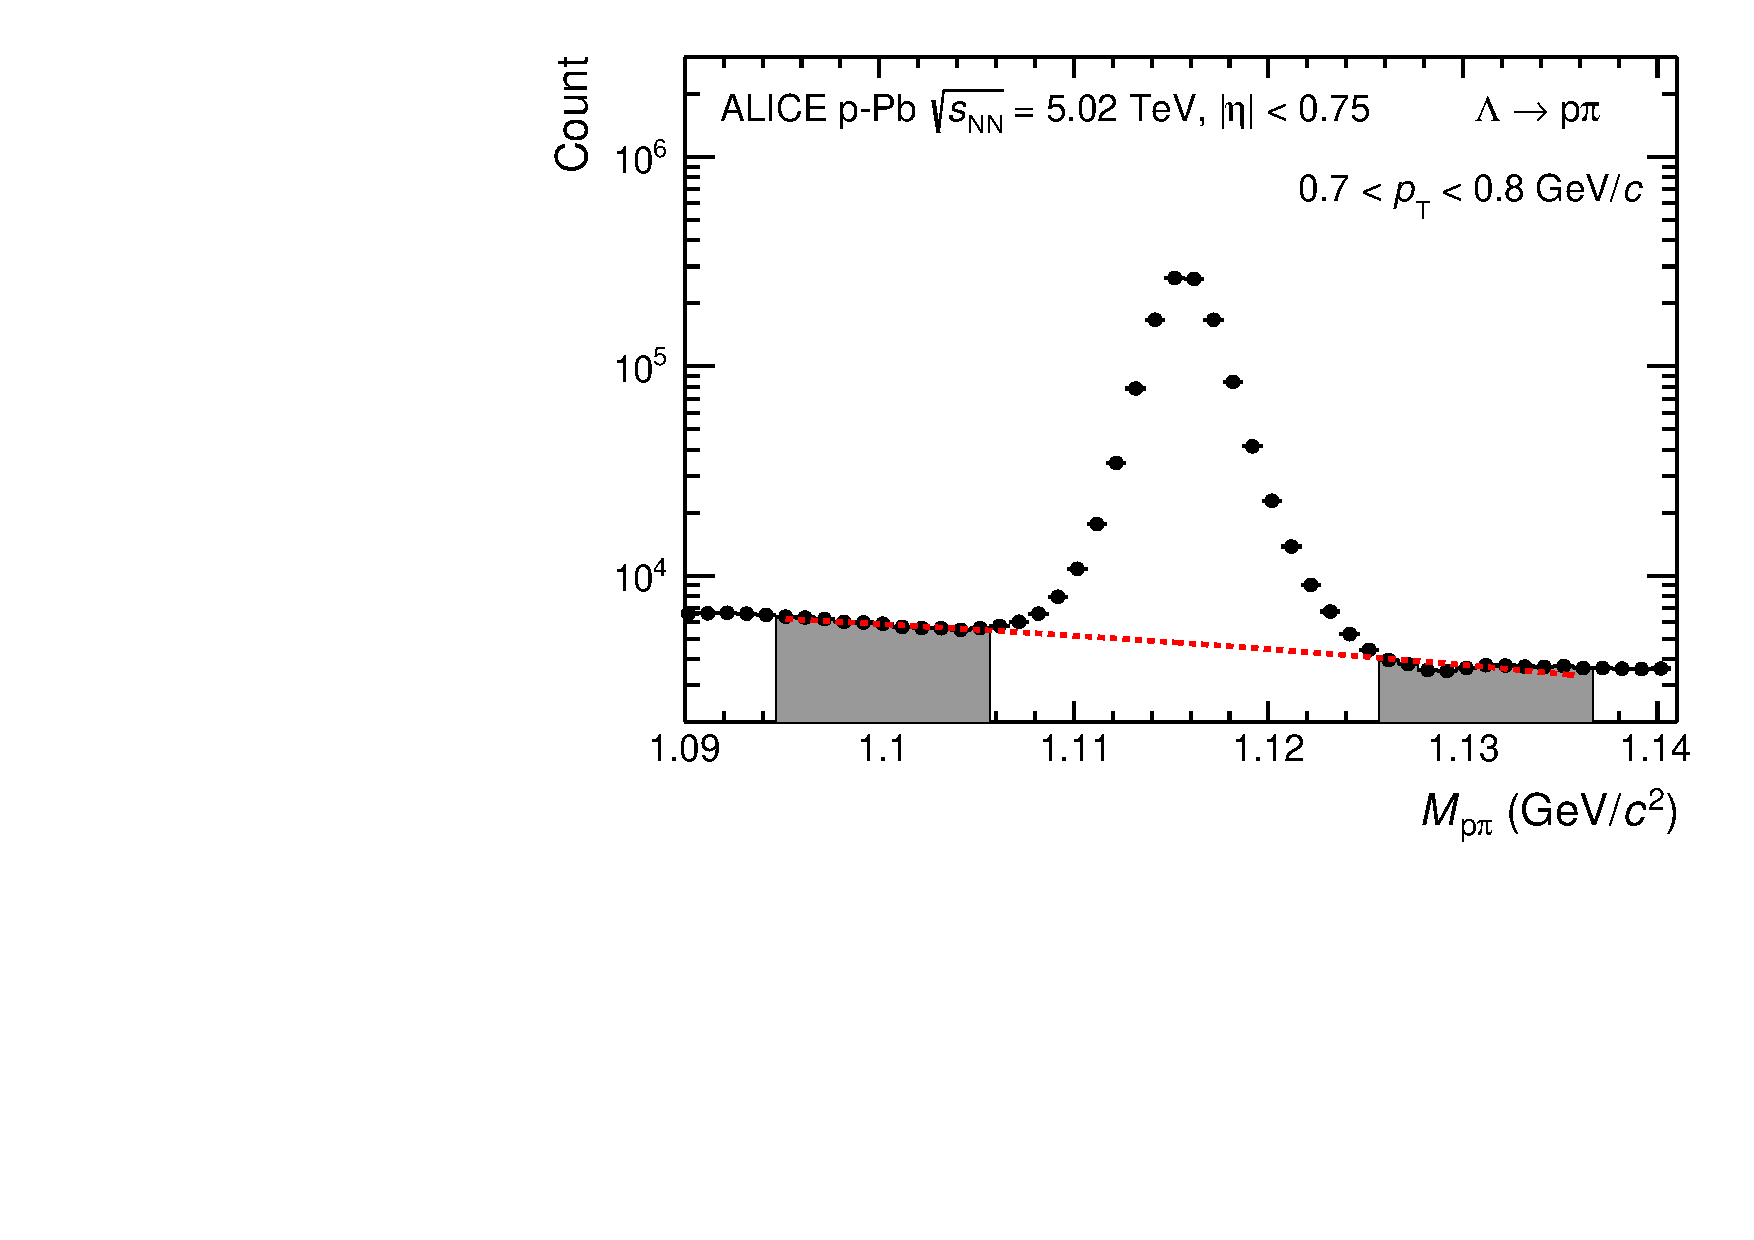
\includegraphics[width=.49\textwidth]{cf01_2}
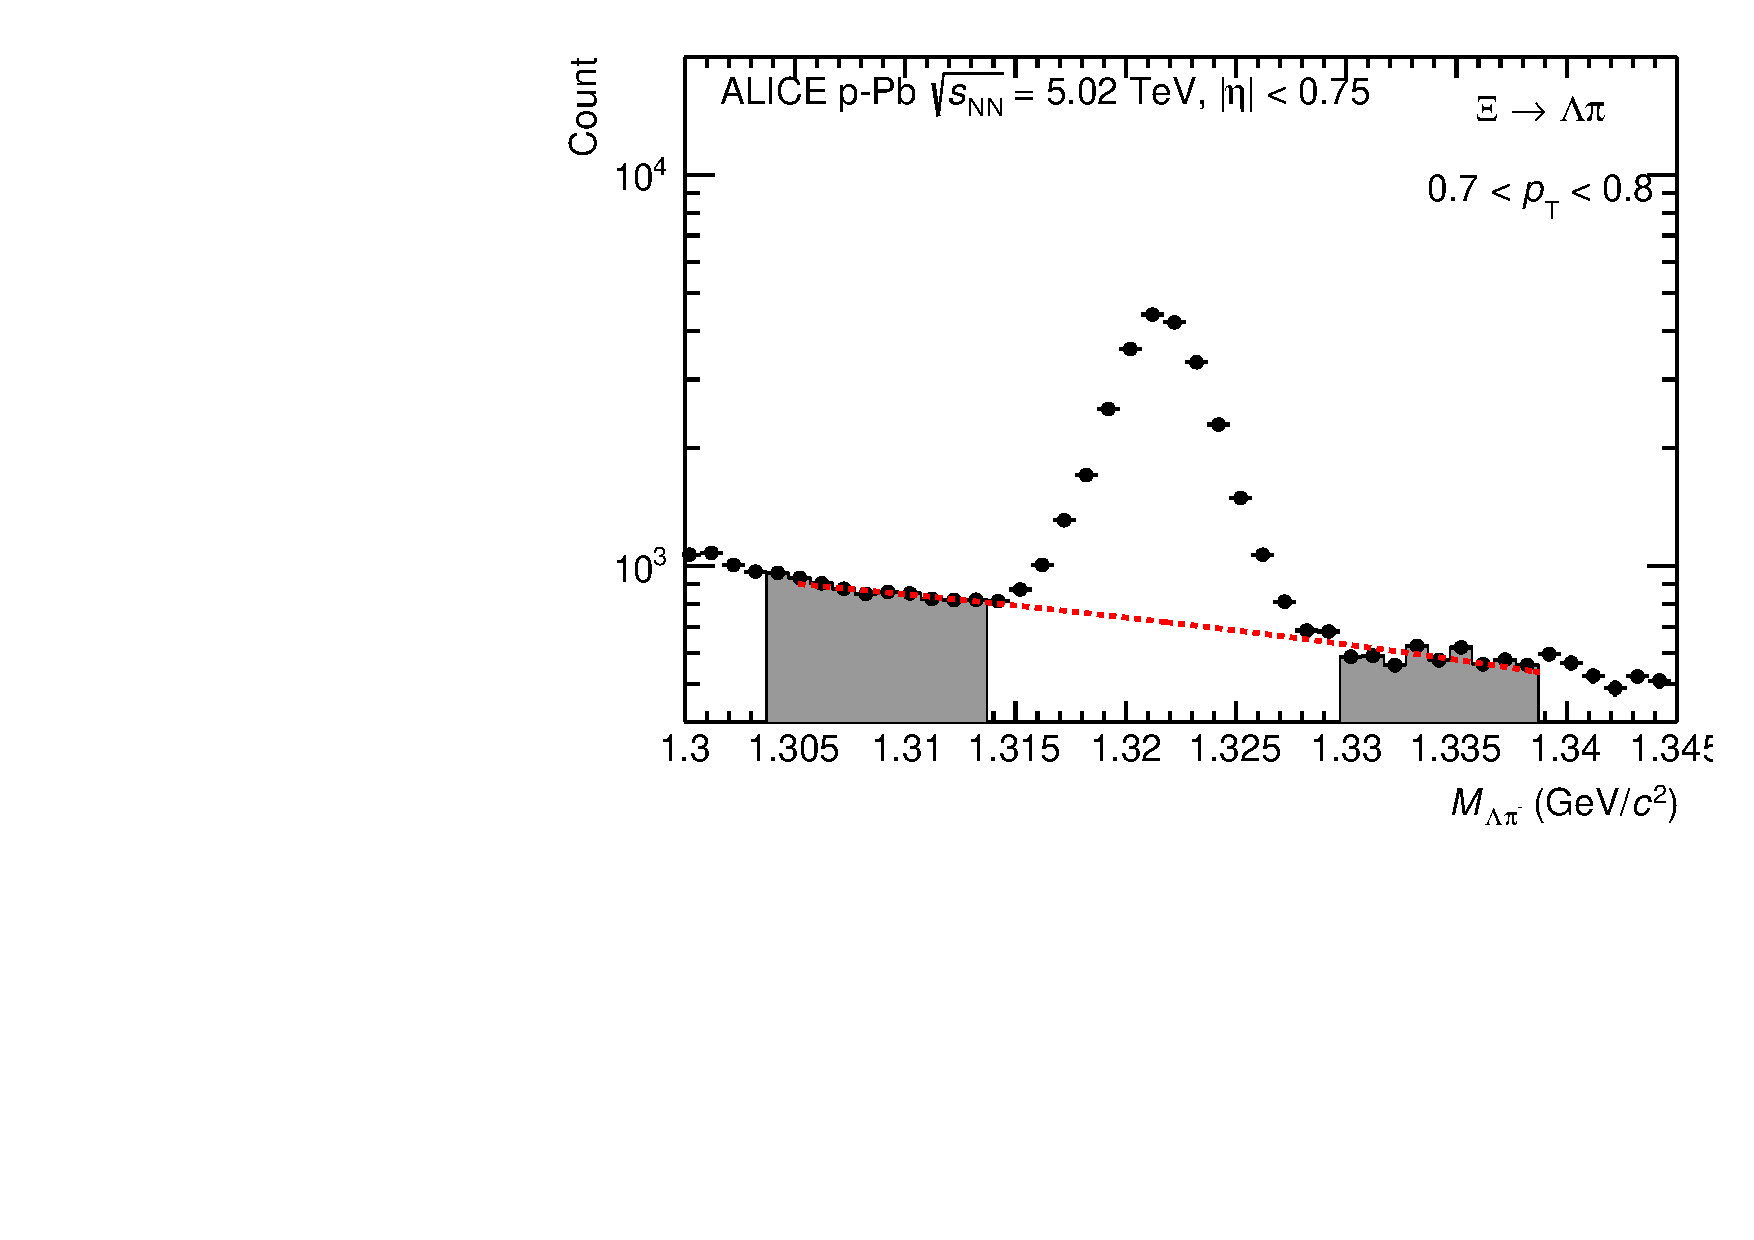
\includegraphics[width=.49\textwidth]{cf01_3}
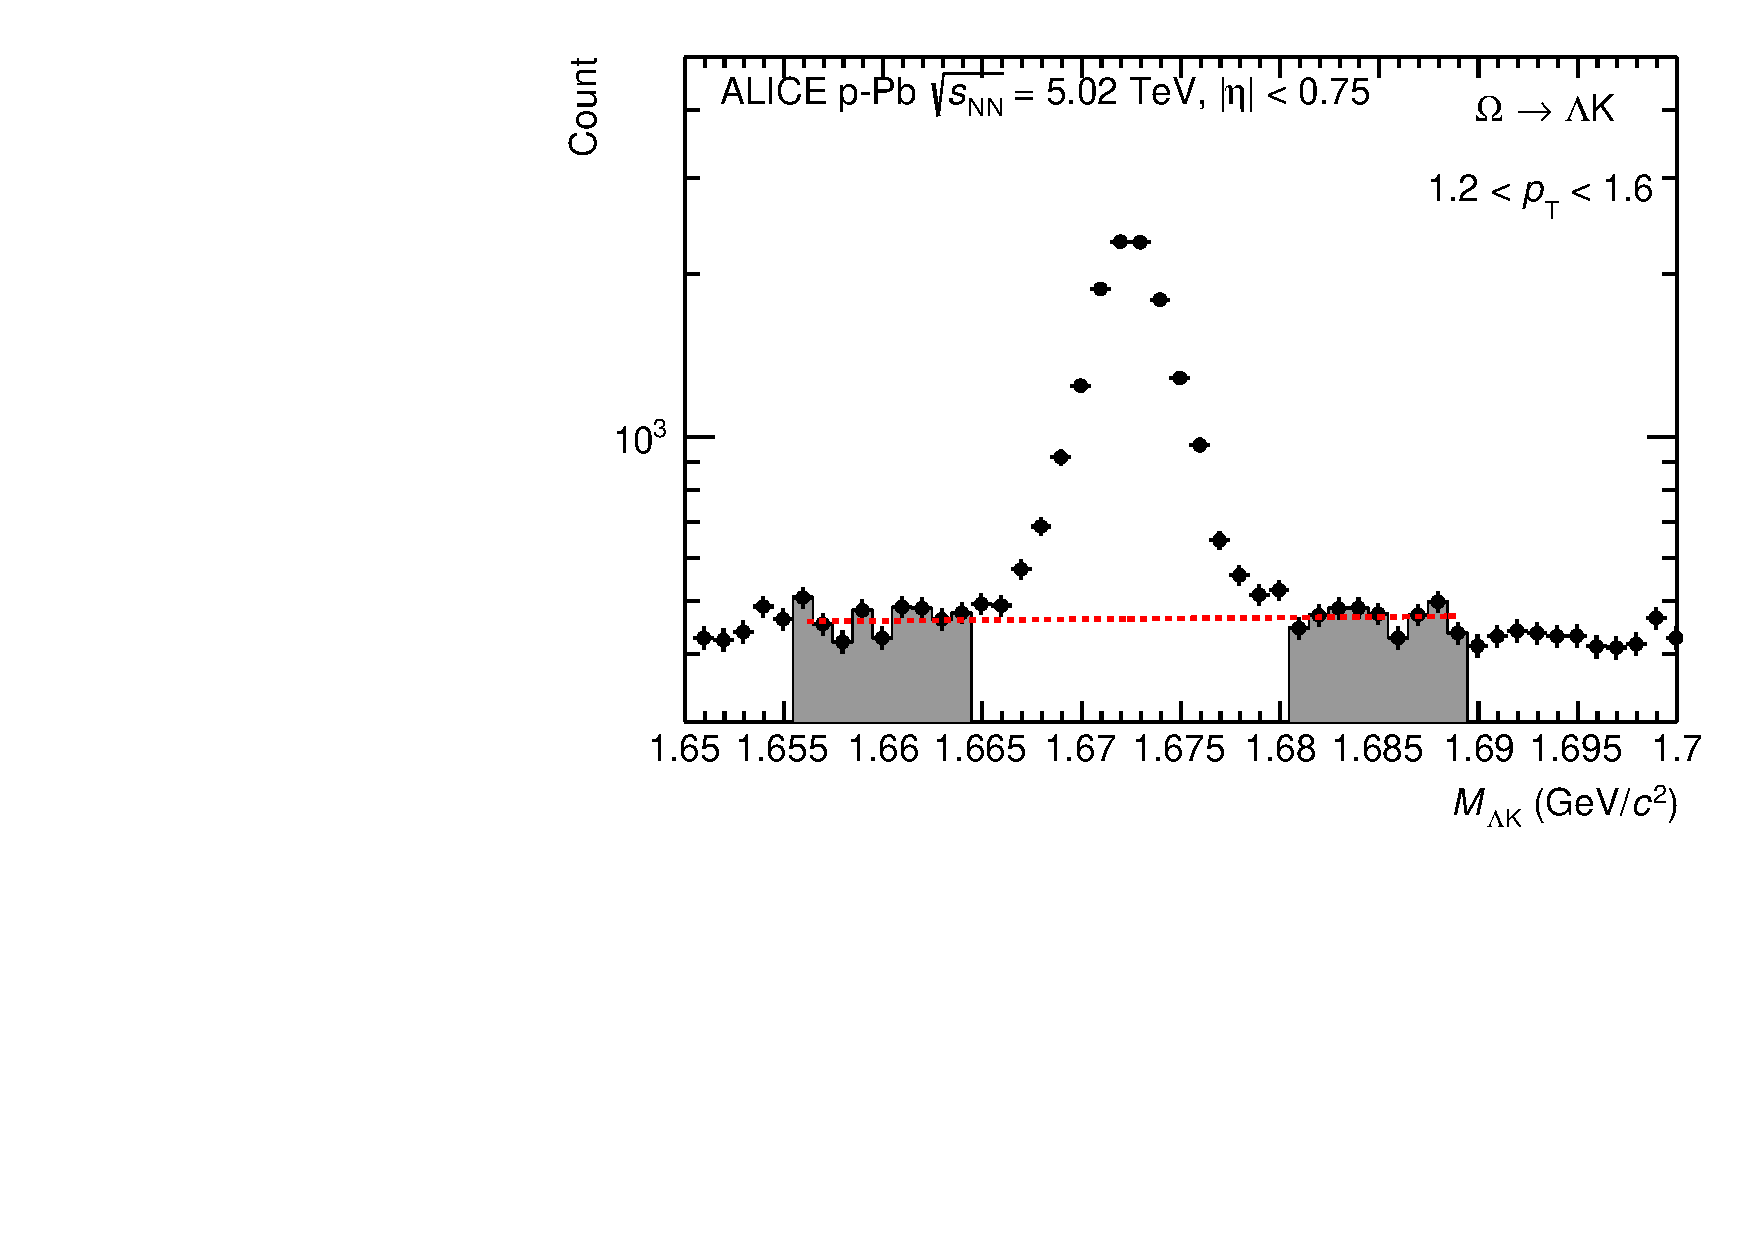
\includegraphics[width=.49\textwidth]{cf01_4}
\caption{Invariant mass distribution for $\kzero$, $\lmb$, $\Xi$ and $\Omega$ in different $\pT$ intervals in MB \pPb collisions at \fivenn. The candidates are reconstructed in $|\eta|<0.75$.
The grey areas are used for background estimation applied in the signal extraction in the bin counting procedure.}
\label{fig:InvM}
\end{center}
\end{figure}

\subsection{Matching of strange particles to jets and underlying event}%
\label{sec:ParJetMatch}

The strategy of matching the (multi-)strange particles with jets follows those presented in earlier work~\cite{Acharya:2021oaa}.
The matching is done on a geometrical basis according to the distance variable defined in Eq.~\ref{eq:DParJet}.
\begin{equation}
d(\mathrm{particle, jet}) = \sqrt{(\eta_\mathrm{particle} -\eta_{\rm jet})^{2} + (\varphi_\mathrm{particle} -\varphi_{\rm jet})^{2}}
\label{eq:DParJet}
\end{equation}
If the distance between the particle candidate and the jet ($d$) is smaller than a pre-defined maximum distance ($D_\mathrm{max}$ = 0.4), the candidate is considered to be inside the jet cone (JC).
The raw yields in JC are not only composed of the hadrons produced via jet fragmentation (JE), but also from hadrons from the underlying event (UE) defined as the sum of all particles which are not produced via hard parton fragmentation.
The UE contribution is estimated by perpendicular cone (PC) yields.
The PC indicates the cone in the $\eta$--$\varphi$ space located at the perpendicular direction with respect to the jet axis at the same $\eta$.
In addition, the acceptance selections of inclusive (regardless of the association between the particle and hard scattering), JC and UE (multi-)strange particles are different in the $\eta$--$\varphi$ plane.
To estimate the contribution from JE the $\pT$-differential particle density (d$\rho$/d$\pT$) is defined in:
\begin{equation}
\begin{split}
{\rm Inclusive:}\qquad & \frac{\dd\rho}{\dd\pT} = \frac{1}{N_{\rm ev}}\times\frac{1}{\Delta\eta\Delta\varphi}\times\frac{\dd N}{\dd\pT}, \\
{\rm JC:}\qquad & \frac{\dd\rho}{\dd\pT} = \frac{1}{N_{\rm ev}^{\rm jet}} \times\frac{1}{A_{\rm jet}}\times\frac{\dd N}{\dd\pT}, \\
{\rm PC:}\qquad & \frac{\dd\rho}{\dd\pT} = \frac{1}{N_{\rm ev}^{\rm jet}} \times\frac{1}{A_{\rm PC}}\times\frac{\dd N}{\dd\pT}. \\
\end{split}
\label{eq:normalize}
\end{equation}
Where the $\Delta\eta\Delta\varphi$ is the acceptance in pseudo-rapidity and azimuthal angle, the $A_\mathrm{jet}$ is the jet area, and the $A_\mathrm{PC}$ is the perpendicular cone area.
The density of particles within jet (JE) can be defined as: ${\rm JE = JC - PC}$.

\subsection{Corrections for strange particles reconstruction and feed-down}
\label{SubSec:Correction}
The reconstruction efficiency of each particle is obtained from Monte Carlo simulated data.
For this purpose PYTHIA 8.2~\cite{Sjostrand:2014zea} and DPMJet~\cite{Roesler:2000he} in \pp and \pPb collisions are used and the simulated data are propagated through the detector by GEANT 3~\cite{Brun:1994aa} to simulate ALICE detector response.
Due to differences in the experimental acceptance for particles associated with jets and underlying event, the efficiencies of particles are estimated separately for every case~\cite{Acharya:2021oaa}.
Fig.~\ref{fig:EffiJCIncl} shows the difference of reconstruction efficiency of JC particle yields and the inclusive one.

\begin{figure}[!ht]
\begin{center}
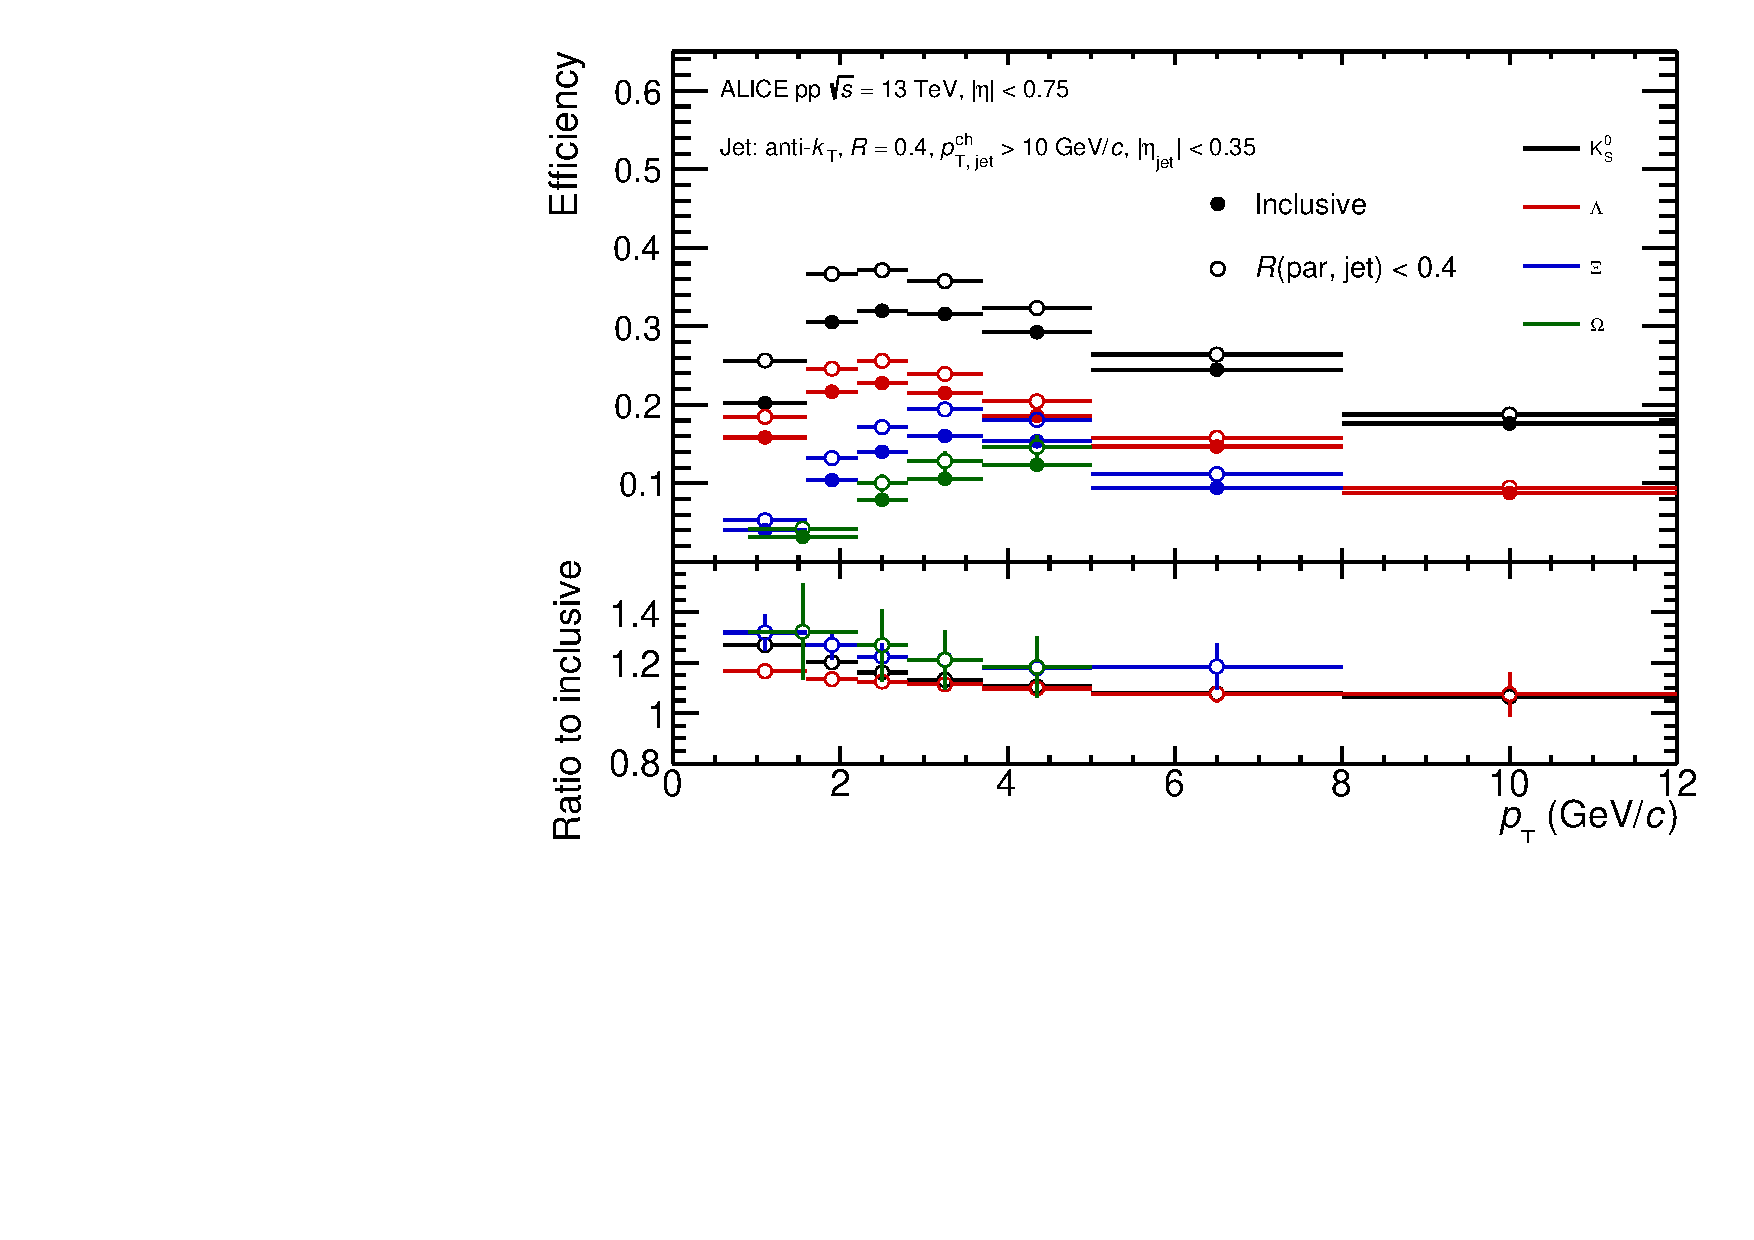
\includegraphics[width=.49\textwidth]{cf02_1}
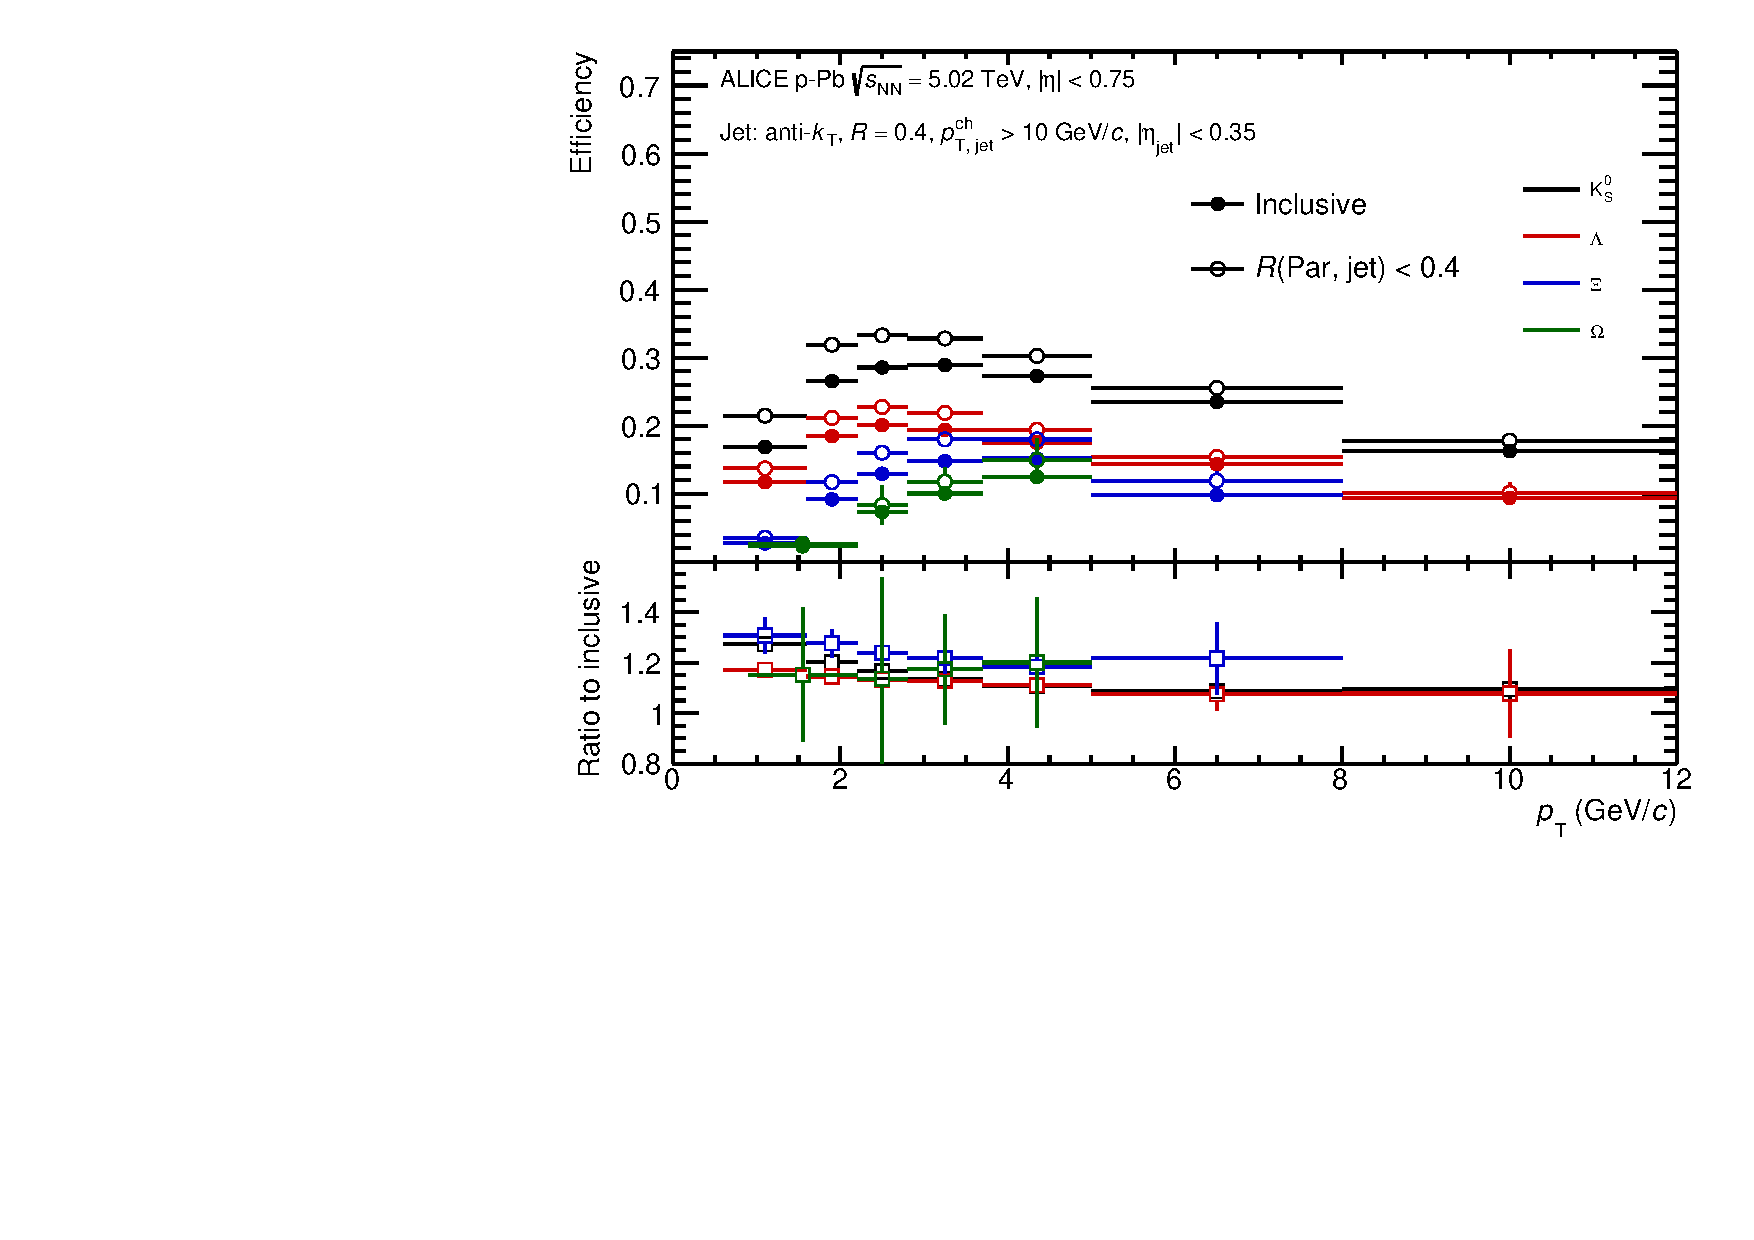
\includegraphics[width=.49\textwidth]{cf02_2}
\end{center}
\caption{Strange particle reconstruction efficiency in \pp collisions at \thirteen (left) and in \pPb collisions at \fivenn (right) for two selections: inside jet cone, $R(\mathrm{par, jet}) < 0.4$ and the inclusive one.}
\label{fig:EffiJCIncl}
\end{figure}

Only the yields for $\lmb$ and $\almb$ are significantly affected by secondary particles coming from the decays of charged and neutral $\Xi$ baryons.
The feed-down fraction is calculated with a data-driven approach~\cite{Abelev:2013haa}.
The detailed of inclusive feed-down method have been introduced in previous ALICE analyses~\cite{Acharya:2019kyh, Acharya:2020uxl, ALICE:2017jyt}.
In particular, the $\lmb$ and $\almb$ in jet and UE feed-down component is usually estimated by inclusive $\Xis$ spectra and PYTHIA simulations~\cite{Acharya:2021oaa}, due to lack of $\Xis$ in jet and UE results.
In this work, the feed-down fraction in jets and UE is computed for each $\pT$ bin by the measured $\Xis$ in jets and UE spectra, thereby assuming that the production rates of charged and neutral $\Xi$ are equal.
Figure~\ref{fig:FdFrac} shows the results of feed-down fraction in JC and the inclusive one.

\begin{figure}[!ht]
\begin{center}
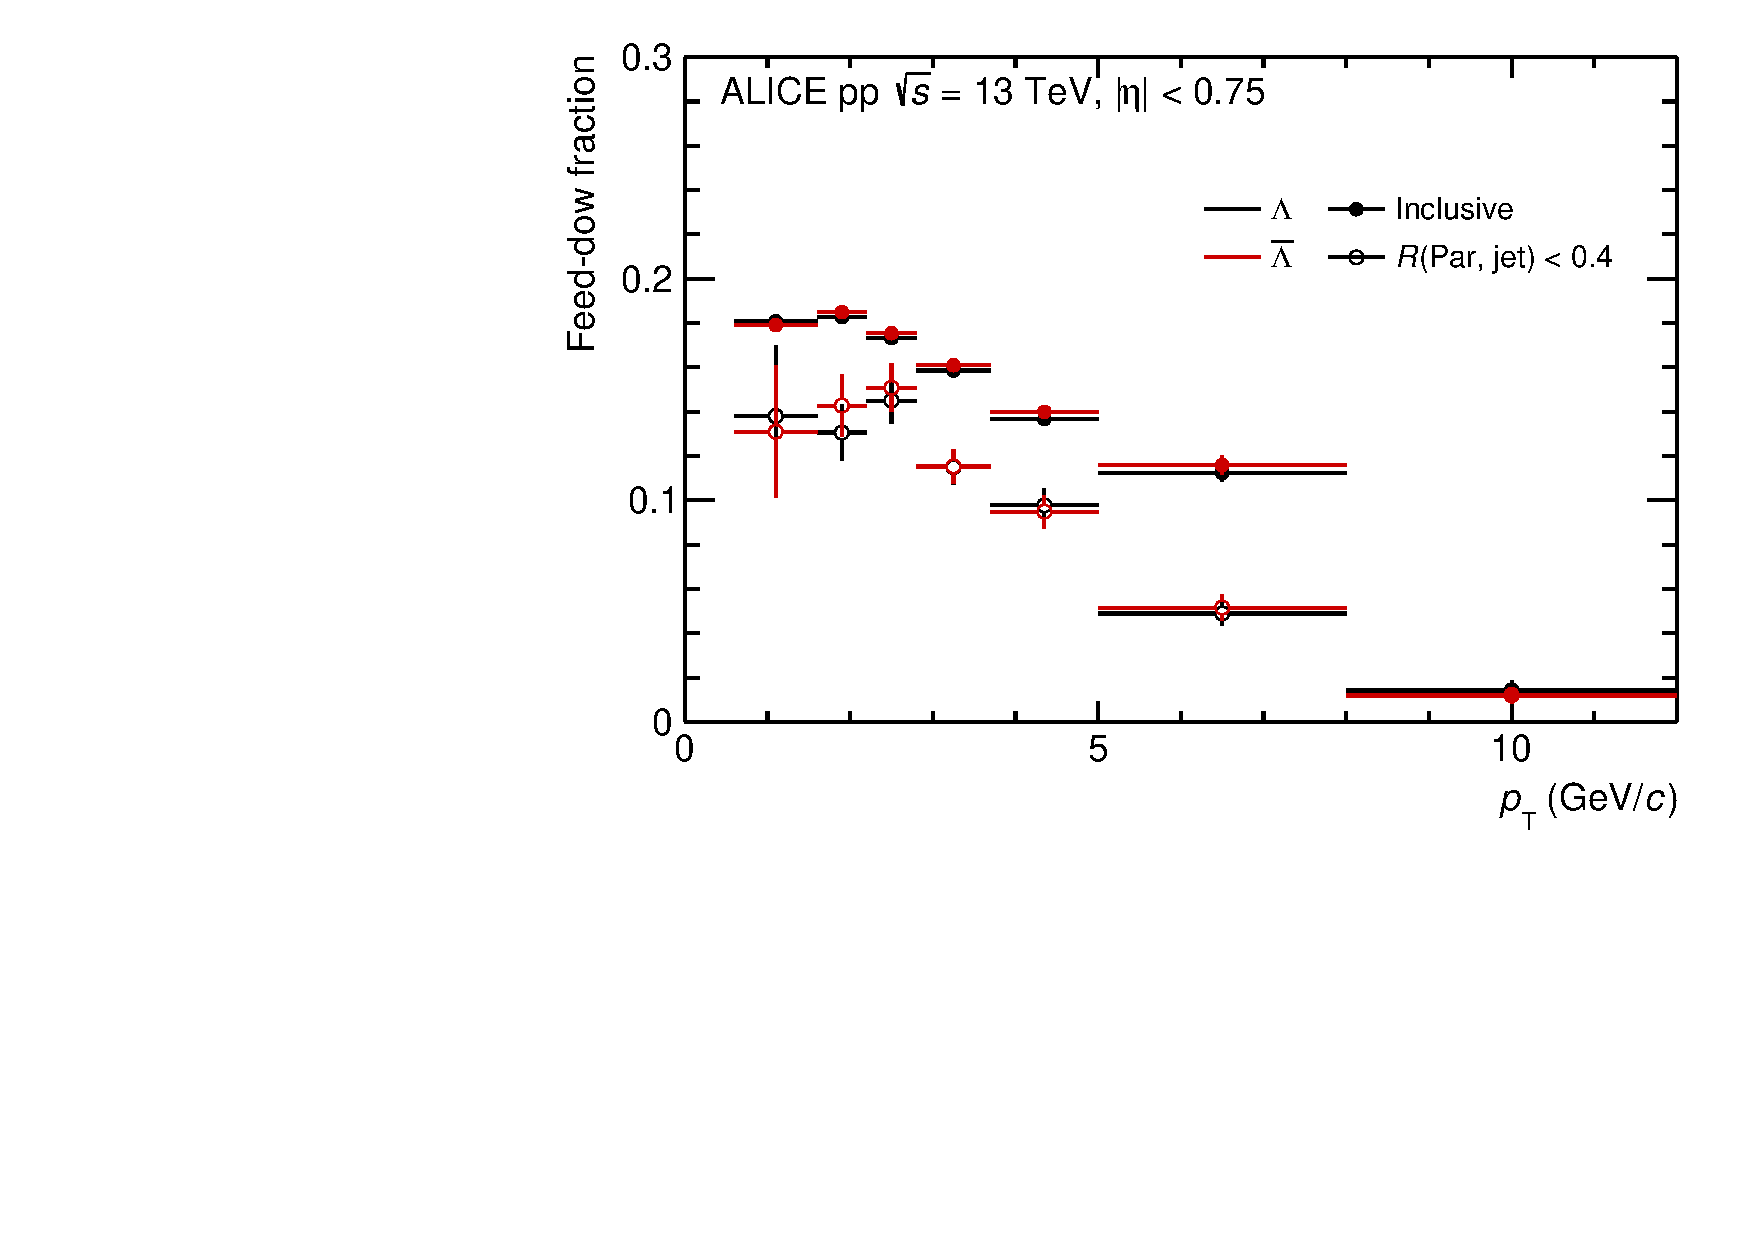
\includegraphics[width=.49\textwidth]{cf03_1}
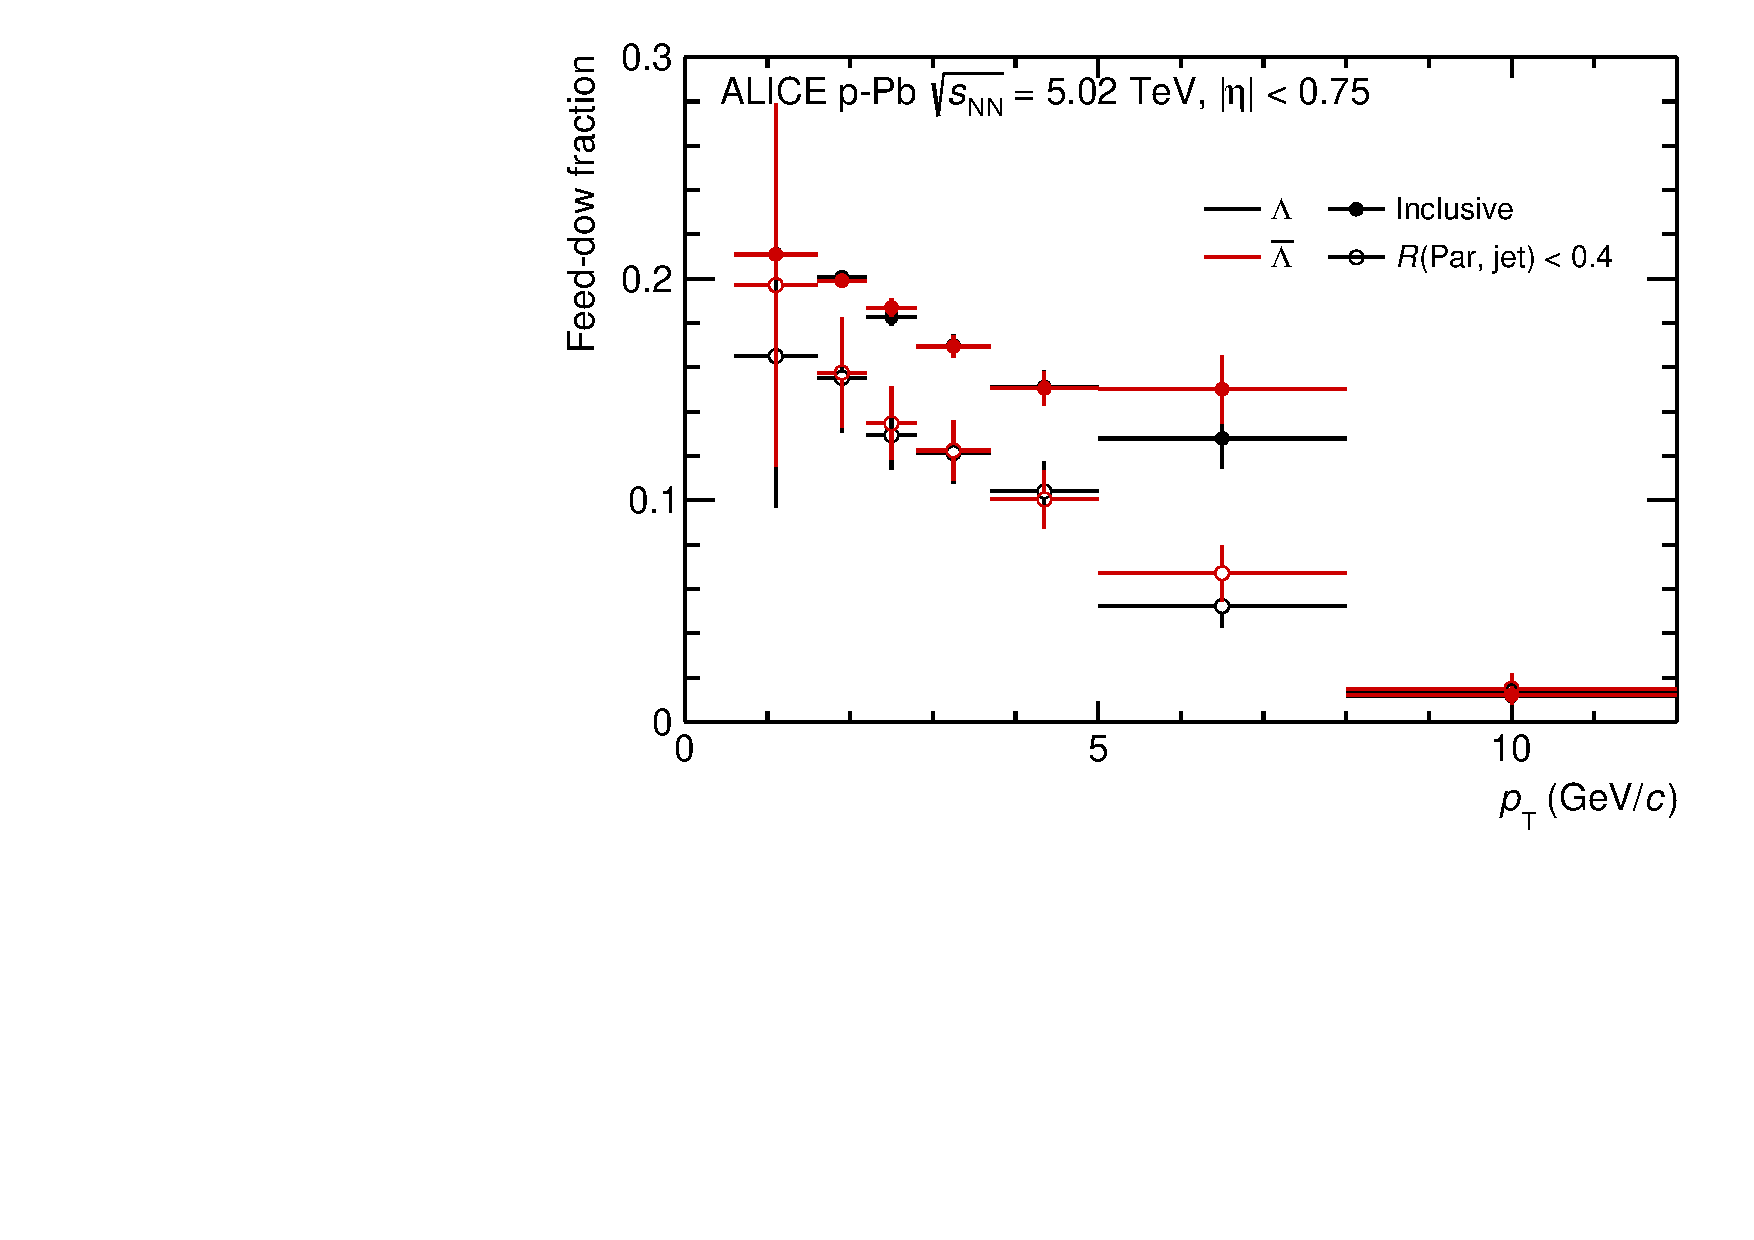
\includegraphics[width=.49\textwidth]{cf03_2}
\end{center}
\caption{Fraction of $\lmb$ spectra removed due to feed-down subtraction of charged and neutral $\Xi$}
\label{fig:FdFrac}
\end{figure}

\subsection{Systematic uncertainties}
\label{sec:SysUncer}
Total systematic uncertainty, for $\kzero$, $\lmb$, $\almb$, $\Xis$ and $\Oms$ yields have been estimated separately in each $\pT$ interval.
Individual settings are loosened and tightened, in order to measure changes in the signal loss correction.
The main sources of the systematic uncertainty in this measurements are related to the knowledge of detector materials, track selections, particle identification, proper lifetime, topological selection and signal extraction.
All these individual error contributions, which are listed in Tab.~\ref{tab:ppInclUncer}, \ref{tab:pPbInclUncer} are added in quadrature.

\begin{table}[!ht]
\begin{center}
\caption{Main sources and values of the relative systematic uncertainties (\%) of $\kzero$, $\lmb + \almb$, $\X + \Ix$ and $\Om + \Mo$ in \pp collisions at \thirteen.
The values are reported for low, intermediate and high $\pT$.}
\label{tab:ppInclUncer}
\begin{tabularx}{\textwidth}{@{} lCCCCCCCCCCCC @{}}
\toprule
\textbf{Uncertainty source} & \multicolumn{3}{c}{\textbf{$\kzero$}}
                            & \multicolumn{3}{c}{\textbf{$\lmb + \almb$}}
                            & \multicolumn{3}{c}{\textbf{$\X + \Ix$}}
                            & \multicolumn{3}{c}{\textbf{$\Om + \Mo$}} \\
\cmidrule(lr){2-4} \cmidrule(lr){5-7} \cmidrule(lr){8-10} \cmidrule(lr){11-13}
$\pT$ (\GeVc) & 0.6 & 2 &10  & 0.6 & 2 & 10  & 0.6 & 2 & 7   & 1& 2 & 5 \\
\midrule
Detector material & 4 & 4 & 4 & 4 & 4 & 4 & 4 & 4 & 4 & 4 & 4 & 4 \\
Track selection &  1.5 & 1.2 & 0.4 & 0.6 & 1.4 & 1.3 & 2.8 & 0.1 & 0. & 0. & 1.5 & 0.2\\
Particle identification& 0.1& 0.1& 0.1 & 0.3 & 0.2 & 1.1 & 1.9 & 1.7 & 2.4& 3.9& 8.7& 6.\\
Proper lifetime& 0& 0.1& 0& 2.1& 0.4& 0& -& -& -& -& -& -\\
Topological& 0.2& 1.4& 0& 3.9& 0.8& 3.9& 0.6& 0.9& 1.& 2.8& 5.4& 2.4\\
Signal extraction& 0.8& 1.1& 1.1& 0.3& 0.5& 1.7& 3. & 1.& 0.5& 2.3& 4.6& 3 \\
\midrule
\textbf{Total uncertainty}& 4.4& 4.6& 4.2& 6.1& 4.4& 6.1& 6.1& 4.5& 4.8& 6.7& 12.& 8.2\\
\bottomrule
\end{tabularx}
\end{center}
\end{table}

\begin{table}[!ht]
\begin{center}
\caption{Main sources and values of the relative systematic uncertainties (\%) of $\kzero$, $\lmb + \almb$, $\X + \Ix$ and $\Om + \Mo$ in \pPb collisions at \fivenn.
The values are reported for low, intermediate and high $\pT$ values.}
\label{tab:pPbInclUncer}
\begin{tabularx}{\textwidth}{@{} lCCCCCCCCCCCC @{}}
\toprule
\textbf{Uncertainty source} & \multicolumn{3}{c}{\textbf{\kzero}}
                            & \multicolumn{3}{c}{\textbf{$\lmb + \almb$}}
                            & \multicolumn{3}{c}{\textbf{$\X + \Ix$}}
                            & \multicolumn{3}{c}{\textbf{$\Om + \Mo$}} \\
\cmidrule(lr){2-4} \cmidrule(lr){5-7} \cmidrule(lr){8-10} \cmidrule(lr){11-13}
$\pT$ (\GeVc) & 0.6 & 2 &10  & 0.6 & 2 & 10    & 0.6 & 2 & 7   & 1& 2 & 5 \\
\midrule
Detector material& 0.4 & 0.4 & 0.4 & 0.4 & 0.4 & 0.4 & 0.4 & 0.4 & 0.4 & 0.4 & 0.4 & 0.4 \\
Track selection & 1.4& 1.7& 1.8& 0.2& 1.3& 1.4& 0& 0& 0& 1.3& 2.5& 0\\
Particle identification& 0.1& 0.2& 0.2& 0.3& 0.2& 1& 3.1&  1.2& 0& 8.1& 13.7& 5.9 \\
Proper lifetime & 0& 0& 0& 1.6& 0.3& 0& 0.6& 0.4& 0& 0& 3.3& 0\\
Topological & 4.4& 0.6& 1.9& 3.9& 0.9& 2.7& 1.3& 0& 2.6& 1.2& 4.8& 3.7\\
Signal extraction& 0.3& 2.6& 1.7& 0.6& 0.5& 2.6& 5.1& 0.9& 2.6& 0& 5.2& 0\\
\midrule
\textbf{Total uncertainty}& 6.1& 5.1& 5.1& 5.8& 4.3& 5.8& 7.4& 4.3& 5.4& 9.2& 16.4& 8\\
\bottomrule
\end{tabularx}
\end{center}
\end{table}

\textbf{Material budget.} The effect of the incomplete knowledge of the detector's material budget is evaluated by comparing different Monte Carlo simulations in which the material budget was increased and decreased by $4.5\%$.
This value corresponds to the uncertainty on the determination of the material budget by measuring photon conversions~\cite{Abelev:2014ffa}.
This particular systematic uncertainty is around $4\%$~\cite{Acharya:2020uxl}.

\textbf{Track selection.} To estimate the systematic uncertainty due to the track selection, the analysis has been redone with an increased number of required clusters in the TPC from default 70 points to 80 points.

\textbf{Particle identification.} The TPC $\dEdx$ selection is used to reduce the combinatorial background in the (multi-)strange particle invariant mass distribution.
The number of Gaussian $\sigma$ in the identification of particles using the $\dEdx$ has been varied from $4\sigma$ to $6\sigma$.

\textbf{Proper lifetime selection.} The proper lifetime is defined as $mLc/p$, where $m$ is the mass of the particles, $L$ is the decay length, and $p$ is the particle's momentum.
The selection on the $mLc/p$ is varied within $12$ to $40$~cm for $\kzero$, $20$ to $40$ cm for $\lmb$ $(\almb)$, $10$ to $30$ cm for $\Xis$, and $5$ to $15$ cm $\Oms$.

\textbf{Topological selection.} The values of the selection criteria for the topological variables are varied within ranges leading to a maximum variation of $\pm 10\%$ in the raw singal yied around their nominal values.
The observed deviations for each component are summed in quadrature.

\textbf{Signal extraction.} In the same spirit, the signal extraction technique has been tested by varying the widths used to define the ``signal" and ``background'' regions, expressed in terms of the number of $\sigma$ as defined in Sec.~\ref{sec:ParRec}.
In particular the width of the peak region has been varied from the standard $6\sigma$ to $7\sigma$, $5\sigma$ and $4\sigma$ for \Vzero particles and  $3\sigma$ to $4\sigma~(3.5\sigma)$ and $2.5\sigma$ for $\Xi(\Omega)$.

The additional systematic uncertainty sources associated with particle yield in the jet originate from the UE subtraction estimator and the jet $\pT$ threshold.
The systematic uncertainty due to the UE subtraction is estimated by varying the perpendicular cone radius from the chosen thresholds of 0.4~(PC04) to 0.2~(PC02) and 0.6~(PC06).
From the deviations obtained for different PC cone size, the relative systematic uncertainty of the UE subtraction is estimated.
To estimate the effect of jet $\pT$ threshold uncertainty, the analysis is repeated with the jet $\pT$ cut $10\pm 1$~\GeVc.
The systematic uncertainties of particles in jets are added to the list of uncertainties in quadrature.
The values are shown in Table~\ref{tab:ppJEUncer}, \ref{tab:pPbJEUncer}.

The uncertainties of jet cone particle ratios ($\lmb/\kzero$, $\Xi/\kzero$, $\Omega/\kzero$, $\Xi/\lmb$, $\Omega/\lmb$ and $\Omega/\Xi$) also include three sources: the particle reconstruction, UE subtraction and the jet $\pT$ threshold.
The particle reconstruction uncertainty is propagated from the particle spectra.
Uncertainties related to UE subtraction and jet $\pT$ threshold are obtained by varying the same condition as particle spectra in both numerator and denominator of the corresponding ratios.

\begin{table}[!ht]
\begin{center}
\caption{Main sources and values of the relative systematic uncertainties (\%) of particle $\pT$-differential density ($\kzero$, $\lmb + \almb$, $\X + \Ix$ and $\Om + \Mo$) and particle ratios ($\lmb/\kzero$, $\Xi/\kzero$, $\Omega/\kzero$, $\Xi/\lmb$, $\Omega/\lmb$ and $\Omega/\Xi$) in JE in \pp collisions at \thirteen.
The values are reported for low, intermediate and high $\pT$.}
\label{tab:ppJEUncer}
\begin{tabularx}{\textwidth}{@{} lCCCCCCCCCCCC @{}}
\toprule
\textbf{Uncertainty source} & \multicolumn{3}{c}{\textbf{\kzero}}
                            & \multicolumn{3}{c}{\textbf{$\lmb + \almb$}}
                            & \multicolumn{3}{c}{\textbf{$\X + \Ix$}}
                            & \multicolumn{3}{c}{\textbf{$\Om + \Mo$}} \\
\cmidrule(lr){2-4} \cmidrule(lr){5-7} \cmidrule(lr){8-10} \cmidrule(lr){11-13}
$\pT$ (\GeVc) & 0.6 & 2 &10  & 0.6 & 2 & 10    & 0.6 & 2 & 7   & 1& 2 & 5 \\
\midrule
Particle reconstruction& 1.8& 0.25& 0.1& 5.3& 0.6& 0& 6.7& 0.9& 0.1& 6& 1.7& 0.3\\
UE subtraction& 0.1& 0.1& 0.1& 0.1& 0.2& 0.1& 1.5& 0.2& 0.3& 3.6& 1.8& 0.5\\
Jet $\pT$ threshold& 0.6& 3,1& 10.9& 0.6& 1.1& 9.9& 3.5& 2.4& 5& 0& 0& 0\\
\midrule
\textbf{Total uncertainty}& 1.8& 3.1& 10.9& 5.3& 1.2& 9.9& 7.7& 2.6& 5& 7.1& 2.5& 0.6 \\
\bottomrule
\end{tabularx}

\begin{tabularx}{\textwidth}{@{} lCCCCCCCCC @{}}
\toprule
\textbf{Uncertainty source} & \multicolumn{3}{c}{\textbf{$(\lmb + \almb)/(2\kzero)$}}
                            & \multicolumn{3}{c}{\textbf{$(\X + \Ix)/(2\kzero)$}}
                            & \multicolumn{3}{c}{\textbf{$(\Om + \Mo)/(2\kzero)$}} \\
\cmidrule(lr){2-4} \cmidrule(lr){5-7} \cmidrule(lr){8-10}
$\pT$ (\GeVc) & 0.6 & 2 &10  & 0.6 & 2 & 7 & 1 & 2 & 5 \\
\midrule
Particle reconstruction& 2.4& 2.8& 2.5& 3.4& 2.8& 2.8& 6.7& 11.4& 7.3\\
UE subtraction& 0.8& 0.2& 0.4& 3.5& 0.2& 0.1& 10& 4& 2.2\\
Jet $\pT$ threshold& 0.4& 2.3& 1& 1.7& 1.6& 3.6& 1.& 3.3& 6.4\\
\midrule
\textbf{Total uncertainty}& 2.6& 3.7& 2.7& 5.2& 3.3& 4.5& 12.4& 12.5& 10\\
\bottomrule
\end{tabularx}

\begin{tabularx}{\textwidth}{@{} lCCCCCCCCC @{}}
\toprule
\textbf{Uncertainty source} & \multicolumn{3}{c}{\textbf{$(\X + \Ix)/(\lmb + \almb)$}}
                            & \multicolumn{3}{c}{\textbf{$(\Om + \Mo)/(\lmb + \almb)$}}
                            & \multicolumn{3}{c}{\textbf{$(\Om + \Mo)/(\X + \Ix)$}} \\
\cmidrule(lr){2-4} \cmidrule(lr){5-7} \cmidrule(lr){8-10}
$\pT$ (\GeVc) & 0.6 & 2 &7  & 1 & 2 & 5 & 1 & 2 & 5 \\
\midrule
Particle reconstruction& 3.4& 3& 3.2& 6.7& 11.5& 7.5& 6.8& 11.5& 7.4\\
UE subtraction& 4.4& 0.4& 0.2& 12.4& 4.2& 2.3& 7.8& 3.8& 2.7\\
Jet $\pT$ threshold& 0.7& 0.5& 1.9& 0.2& 0.9& 3.5& 0.4& 1.3& 3\\
\midrule
\textbf{Total uncertainty}& 5.6& 3& 3.7& 14.1& 12.2& 8.6& 10.3& 12.1& 8.5\\
\bottomrule
\end{tabularx}
\end{center}
\end{table}

\begin{table}[!ht]
\begin{center}
\caption{Main sources and values of the relative systematic uncertainties (\%) of particle $\pT$-differential density ($\kzero$, $\lmb + \almb$, $\X + \Ix$ and $\Om + \Mo$) and particle ratios ($\lmb/\kzero$, $\Xi/\kzero$, $\Omega/\kzero$, $\Xi/\lmb$, $\Omega/\lmb$ and $\Omega/\Xi$) in JE in \pPb collisions at \fivenn.
The values are reported for low, intermediate and high $\pT$.}
\label{tab:pPbJEUncer}
\begin{tabularx}{\textwidth}{@{} lCCCCCCCCCCCC @{}}
\toprule
\textbf{Uncertainty source} & \multicolumn{3}{c}{\textbf{\kzero}}
                            & \multicolumn{3}{c}{\textbf{$\lmb + \almb$}}
                            & \multicolumn{3}{c}{\textbf{$\X + \Ix$}}
                            & \multicolumn{3}{c}{\textbf{$\Om + \Mo$}} \\
\cmidrule(lr){2-4} \cmidrule(lr){5-7} \cmidrule(lr){8-10} \cmidrule(lr){11-13}
$\pT$ (\GeVc) & 0.6 & 2 &10  & 0.6 & 2 & 10    & 0.6 & 2 & 7   & 1& 2 & 5 \\
\midrule
Particle reconstruction& 5& 0.8& 0& 13.2& 1.5& 0& 24.8& 2.8& 0.3& 8.7& 3.7& 0.9\\
UE subtraction& 0.3& 0.1& 0.1& 0& 0.1& 11.2& 14.1& 0.8& 0.7& 0& 0& 1.2\\
Jet $\pT$ threshold& 0.3& 3.5& 11& 3.2& 1.8& 0.1& 24.9&  3& 4.1& 3.1& 10.7& 7.6\\
\midrule
\textbf{Total uncertainty}& 5& 3.6& 11& 13.5& 2.3& 11.2& 37.9& 4.2& 4.1& 9.3& 11.3& 7.7 \\
\bottomrule
\end{tabularx}

\begin{tabularx}{\textwidth}{@{} lCCCCCCCCC @{}}
\toprule
\textbf{Uncertainty source} & \multicolumn{3}{c}{\textbf{$(\lmb + \almb)/(2\kzero)$}}
                            & \multicolumn{3}{c}{\textbf{$(\X + \Ix)/(2\kzero)$}}
                            & \multicolumn{3}{c}{\textbf{$(\Om + \Mo)/(2\kzero)$}} \\
\cmidrule(lr){2-4} \cmidrule(lr){5-7} \cmidrule(lr){8-10}
$\pT$ (\GeVc) & 0.6 & 2 &10  & 0.6 & 2 & 7 & 1 & 2 & 5 \\
\midrule
Particle reconstruction& 3.2& 3.4& 3.3& 4.7& 3.2& 4& 9.8& 1.5& 7.4\\
UE subtraction& 0.8& 0.1& 0.1& 9.1& 1.8& 1& 4.1& 0& 0.3\\
Jet $\pT$ threshold& 1.4& 2.6& 0.1& 8.6& 2.4& 6& 0.5& 1.5& 0.3\\
\midrule
\textbf{Total uncertainty}& 3.6& 4.3& 3.3& 13.4& 4.4& 7.2& 10.6& 15.1& 7.4\\
\bottomrule
\end{tabularx}

\begin{tabularx}{\textwidth}{@{} lCCCCCCCCC @{}}
\toprule
\textbf{Uncertainty source} & \multicolumn{3}{c}{\textbf{$(\X + \Ix)/(\lmb + \almb)$}}
                            & \multicolumn{3}{c}{\textbf{$(\Om + \Mo)/(\lmb + \almb)$}}
                            & \multicolumn{3}{c}{\textbf{$(\Om + \Mo)/(\X + \Ix)$}} \\
\cmidrule(lr){2-4} \cmidrule(lr){5-7} \cmidrule(lr){8-10}
$\pT$ (\GeVc) & 0.6 & 2 &10  & 0.6 & 2 & 7 & 1 & 2 & 5 \\
\midrule
Particle reconstruction& 4.1& 2.8& 3.7& 9.6& 15& 7.5& 10& 14.9& 8.6\\
UE subtraction& 9.9& 1.9& 0.8& 3.6& 0.1& 0.3& 11& 1.8& 0.1\\
Jet $\pT$ threshold& 2.7& 0.6& 2.6& 0.4& 5& 3& 0.4& 3.8& 1.7\\
\midrule
\textbf{Total uncertainty}& 11.1& 3.4& 4.6& 10.3& 15.8& 8.1& 14.9& 15.5& 8.7\\
\bottomrule
\end{tabularx}
\end{center}
\end{table}

\clearpage

\section{Results and discussion}%
\label{sec:Results}

\subsection{Particles $\pT$-differential density}
\label{subsec:ParPtDensity}

For the strange hadrons discussed in this paper, the ratios of yields for particles and anti-particles are around one within the uncertainties, as expected at these collision energies in the mid-rapidity region~\cite{Acharya:2020uxl, ALICE:2015mpp}.
Therefore, all the $\pT$-differential densities are reported after summing over particle and anti-particles.
The different selections shown below have been introduced in Sec.~\ref{sec:ParJetMatch}, in which also normalization method has been introduced.

\begin{figure}[!ht]
\begin{center}
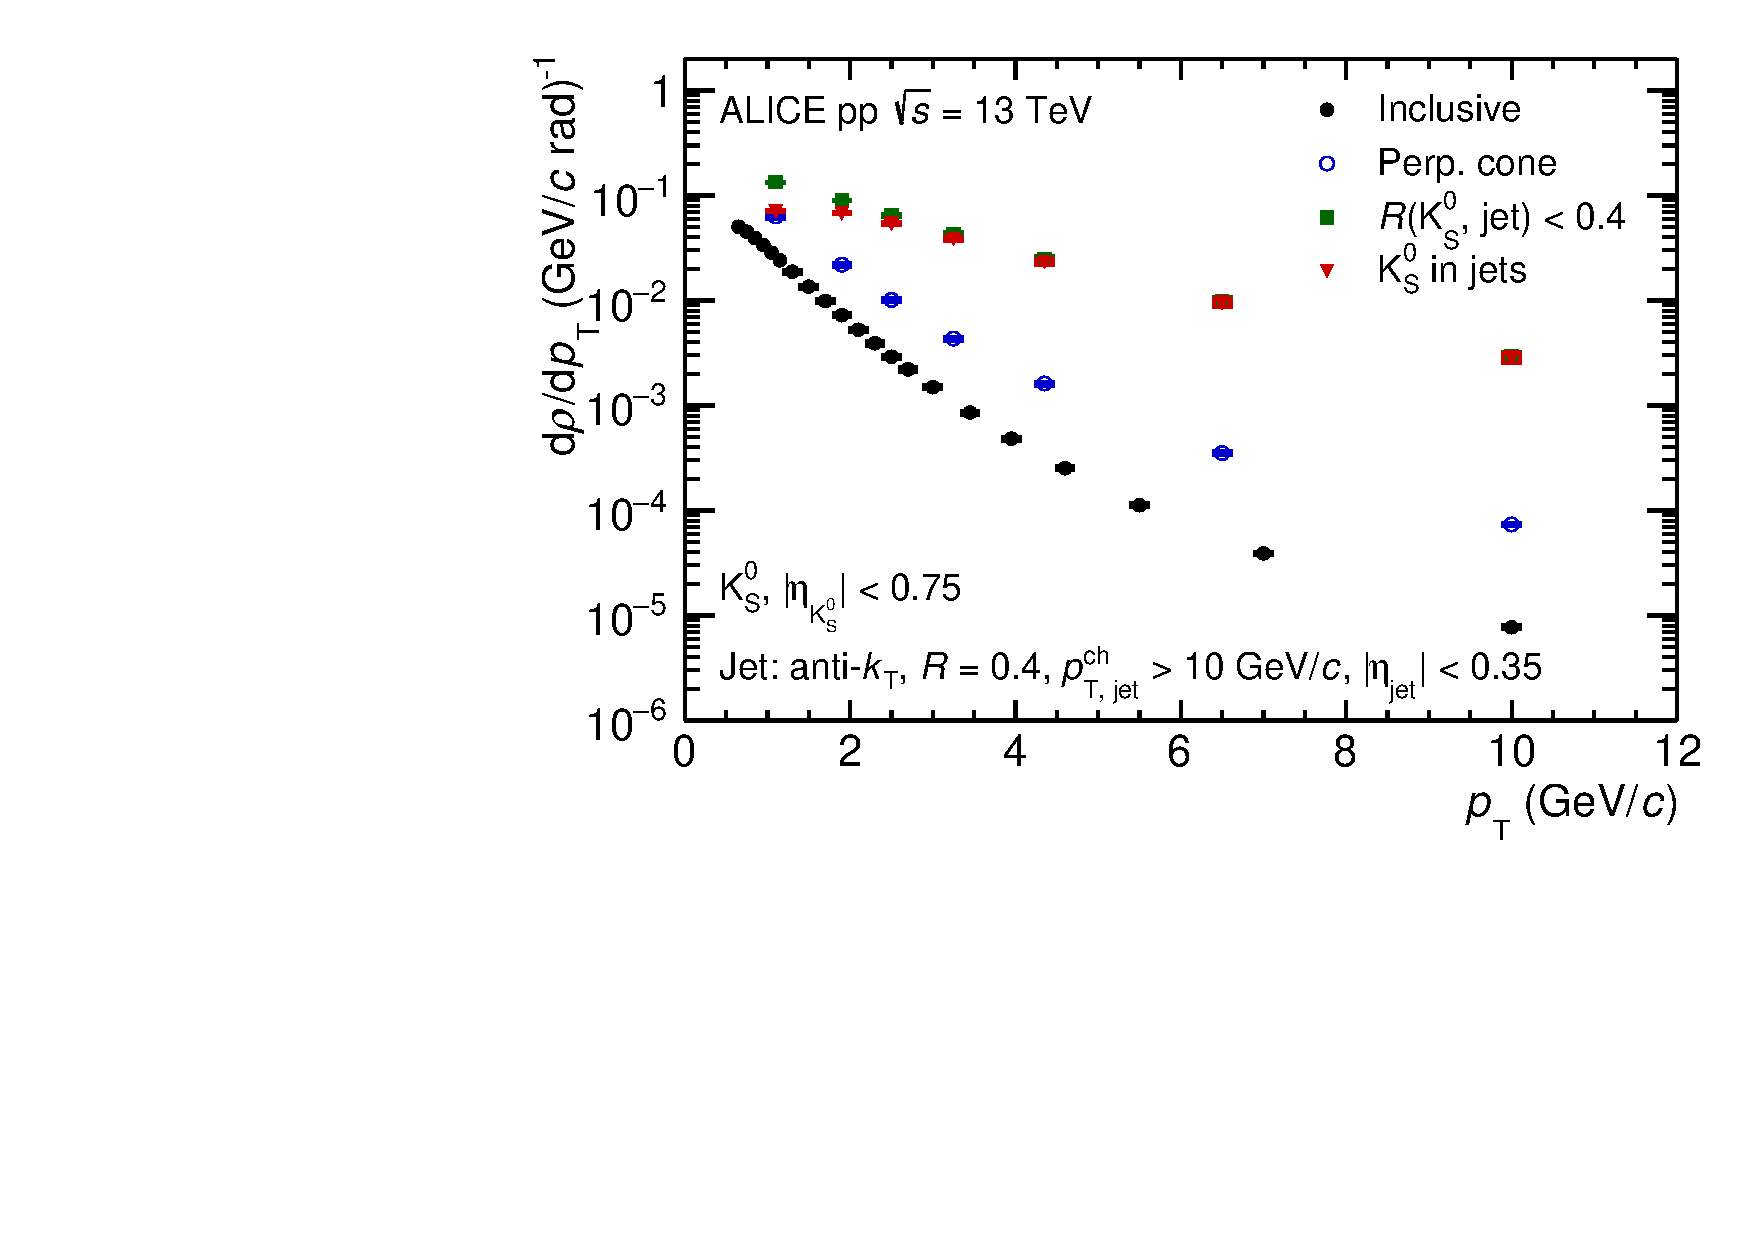
\includegraphics[width=.49\textwidth]{cf04_1}
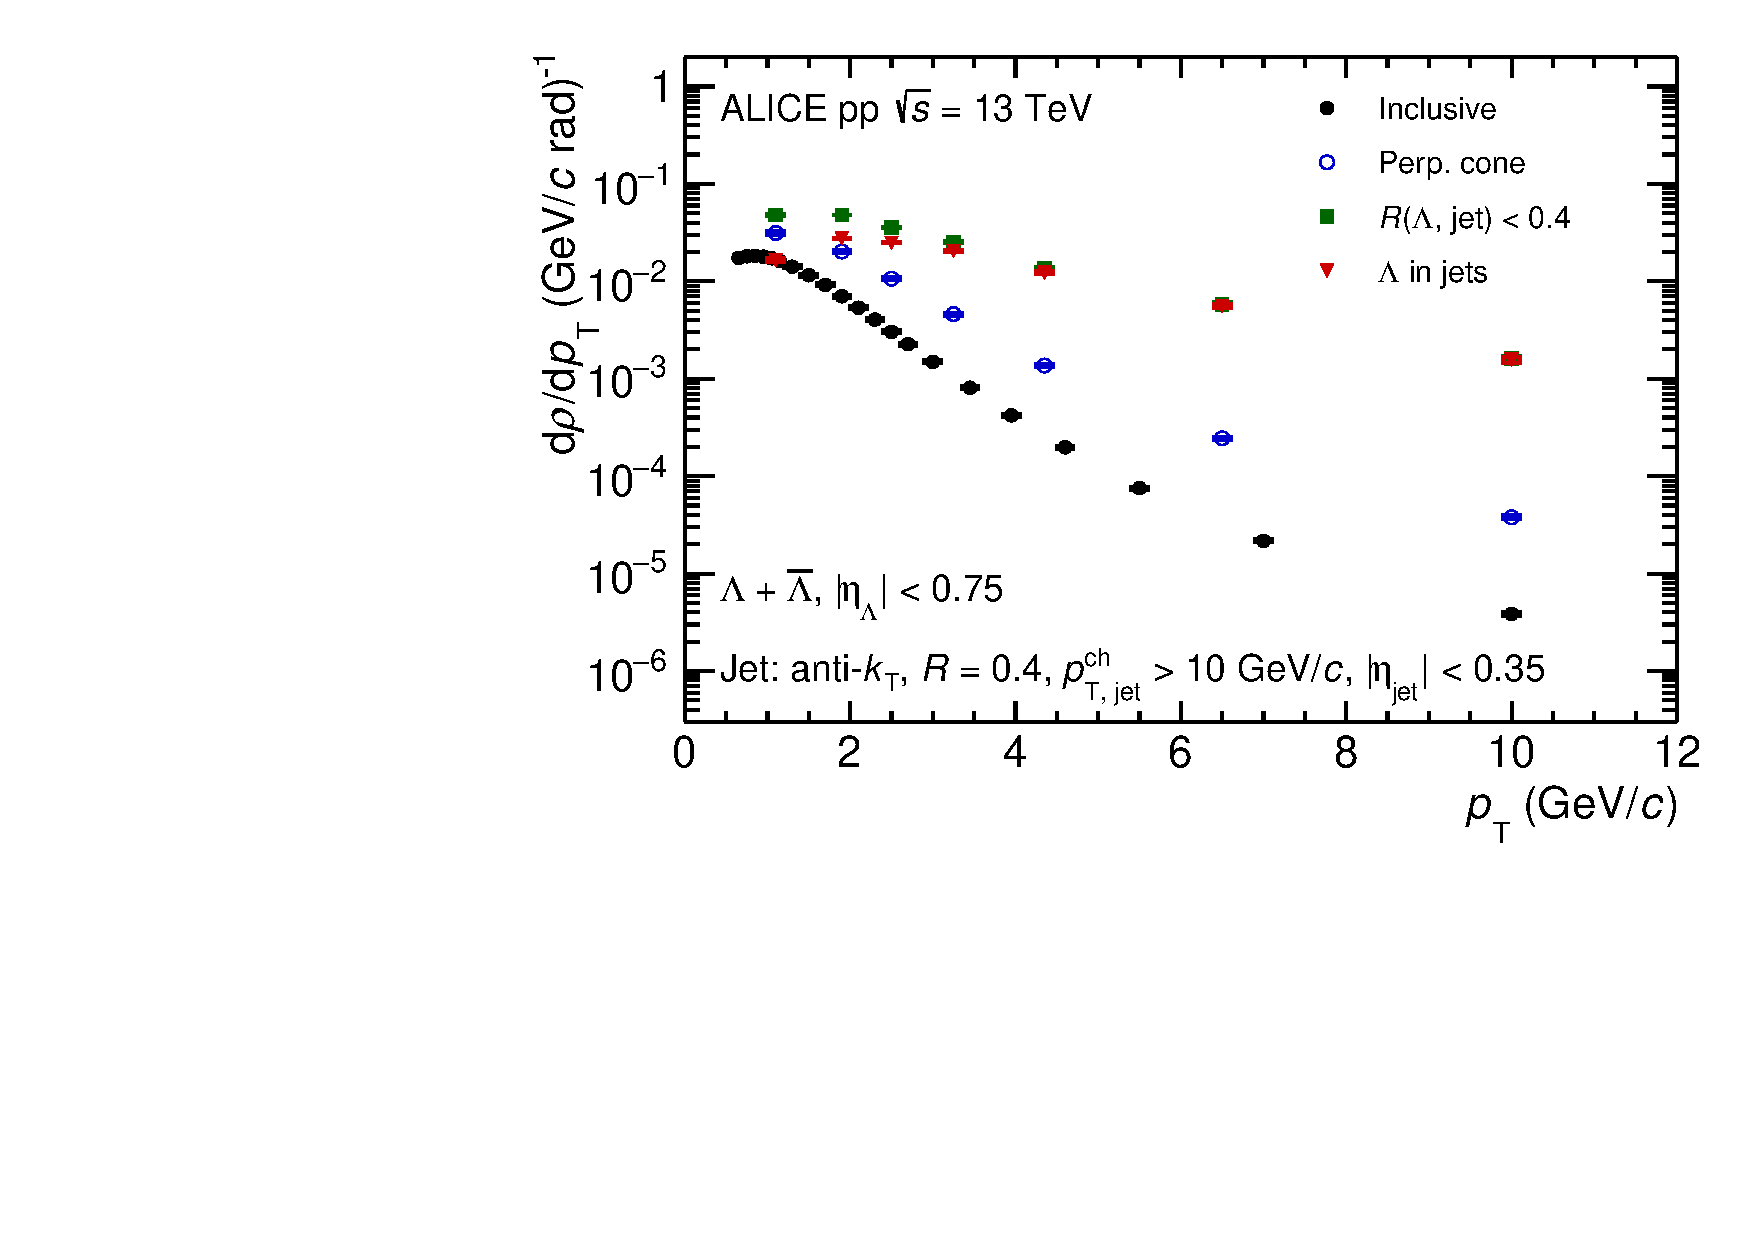
\includegraphics[width=.49\textwidth]{cf04_2}
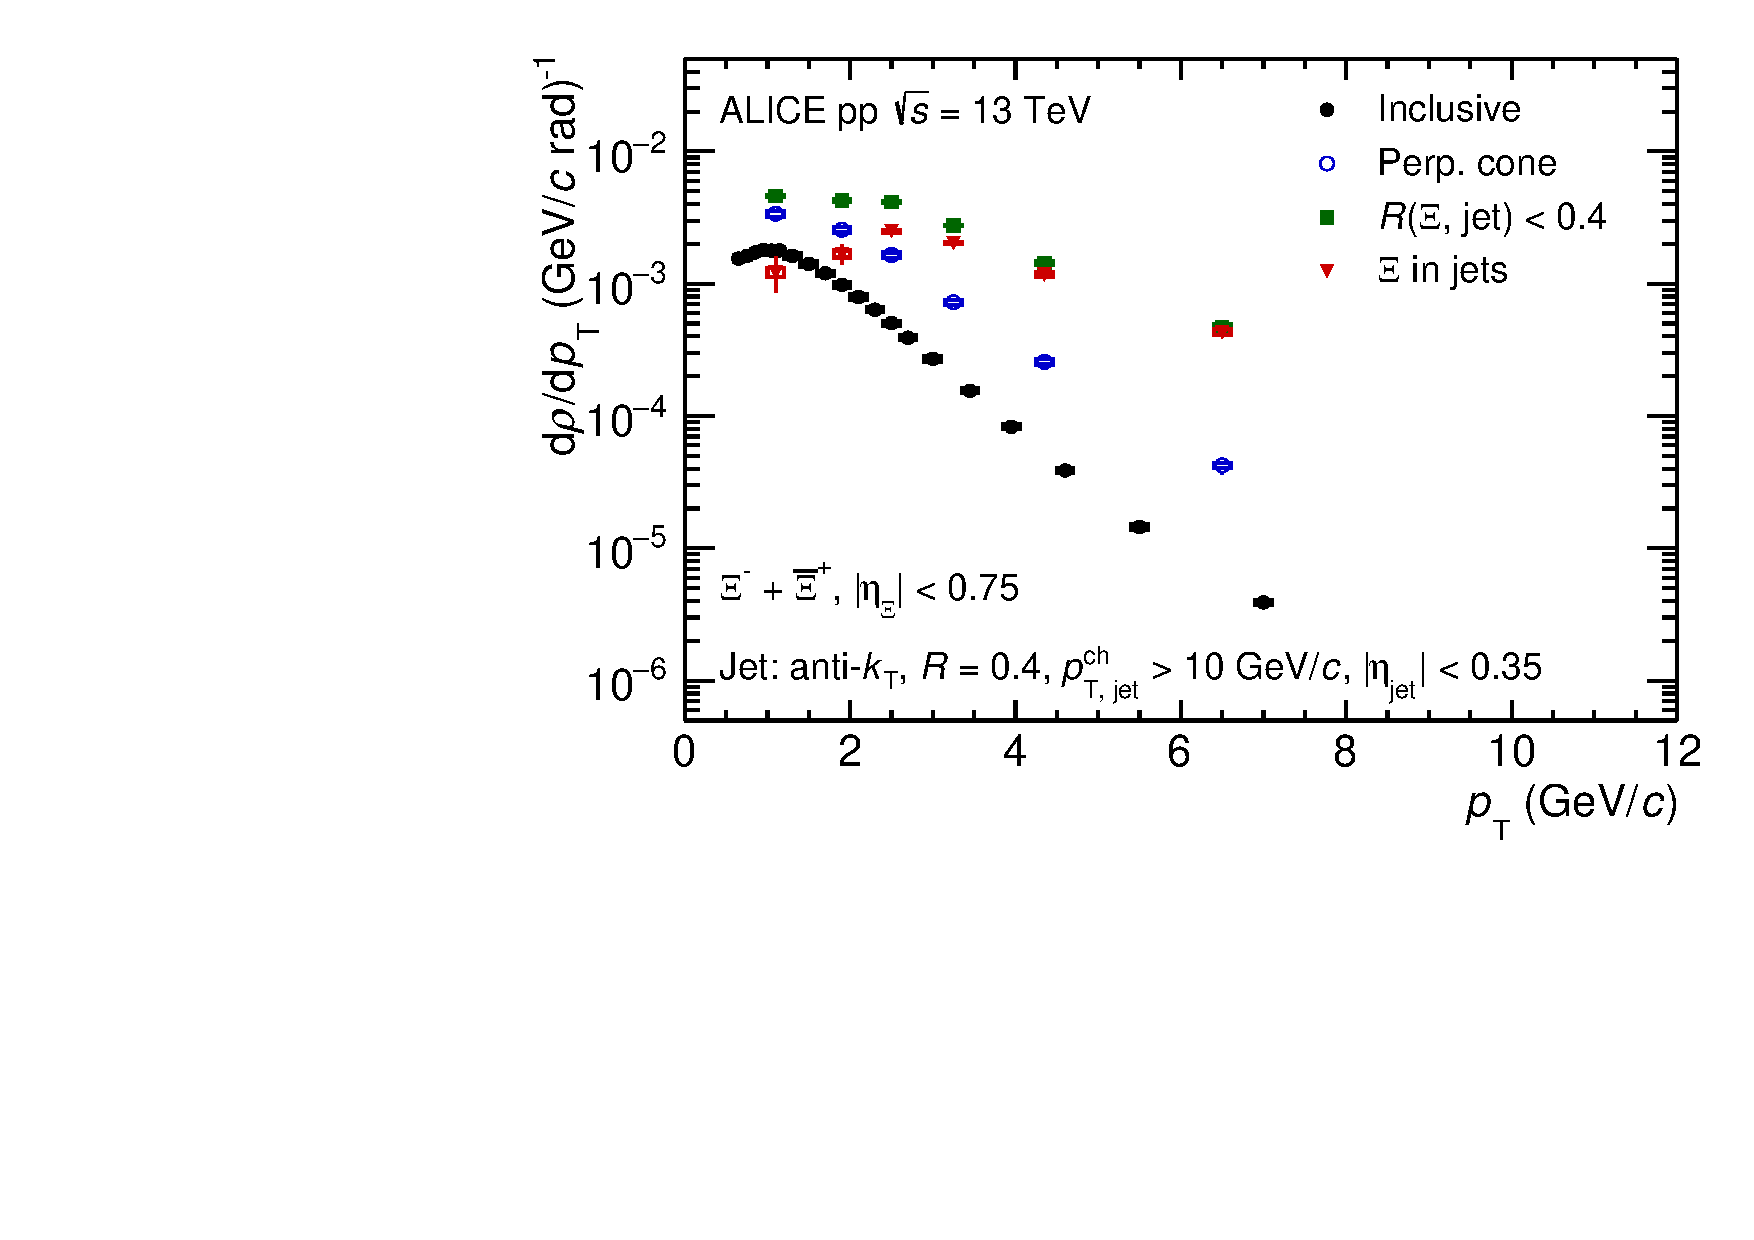
\includegraphics[width=.49\textwidth]{cf04_3}
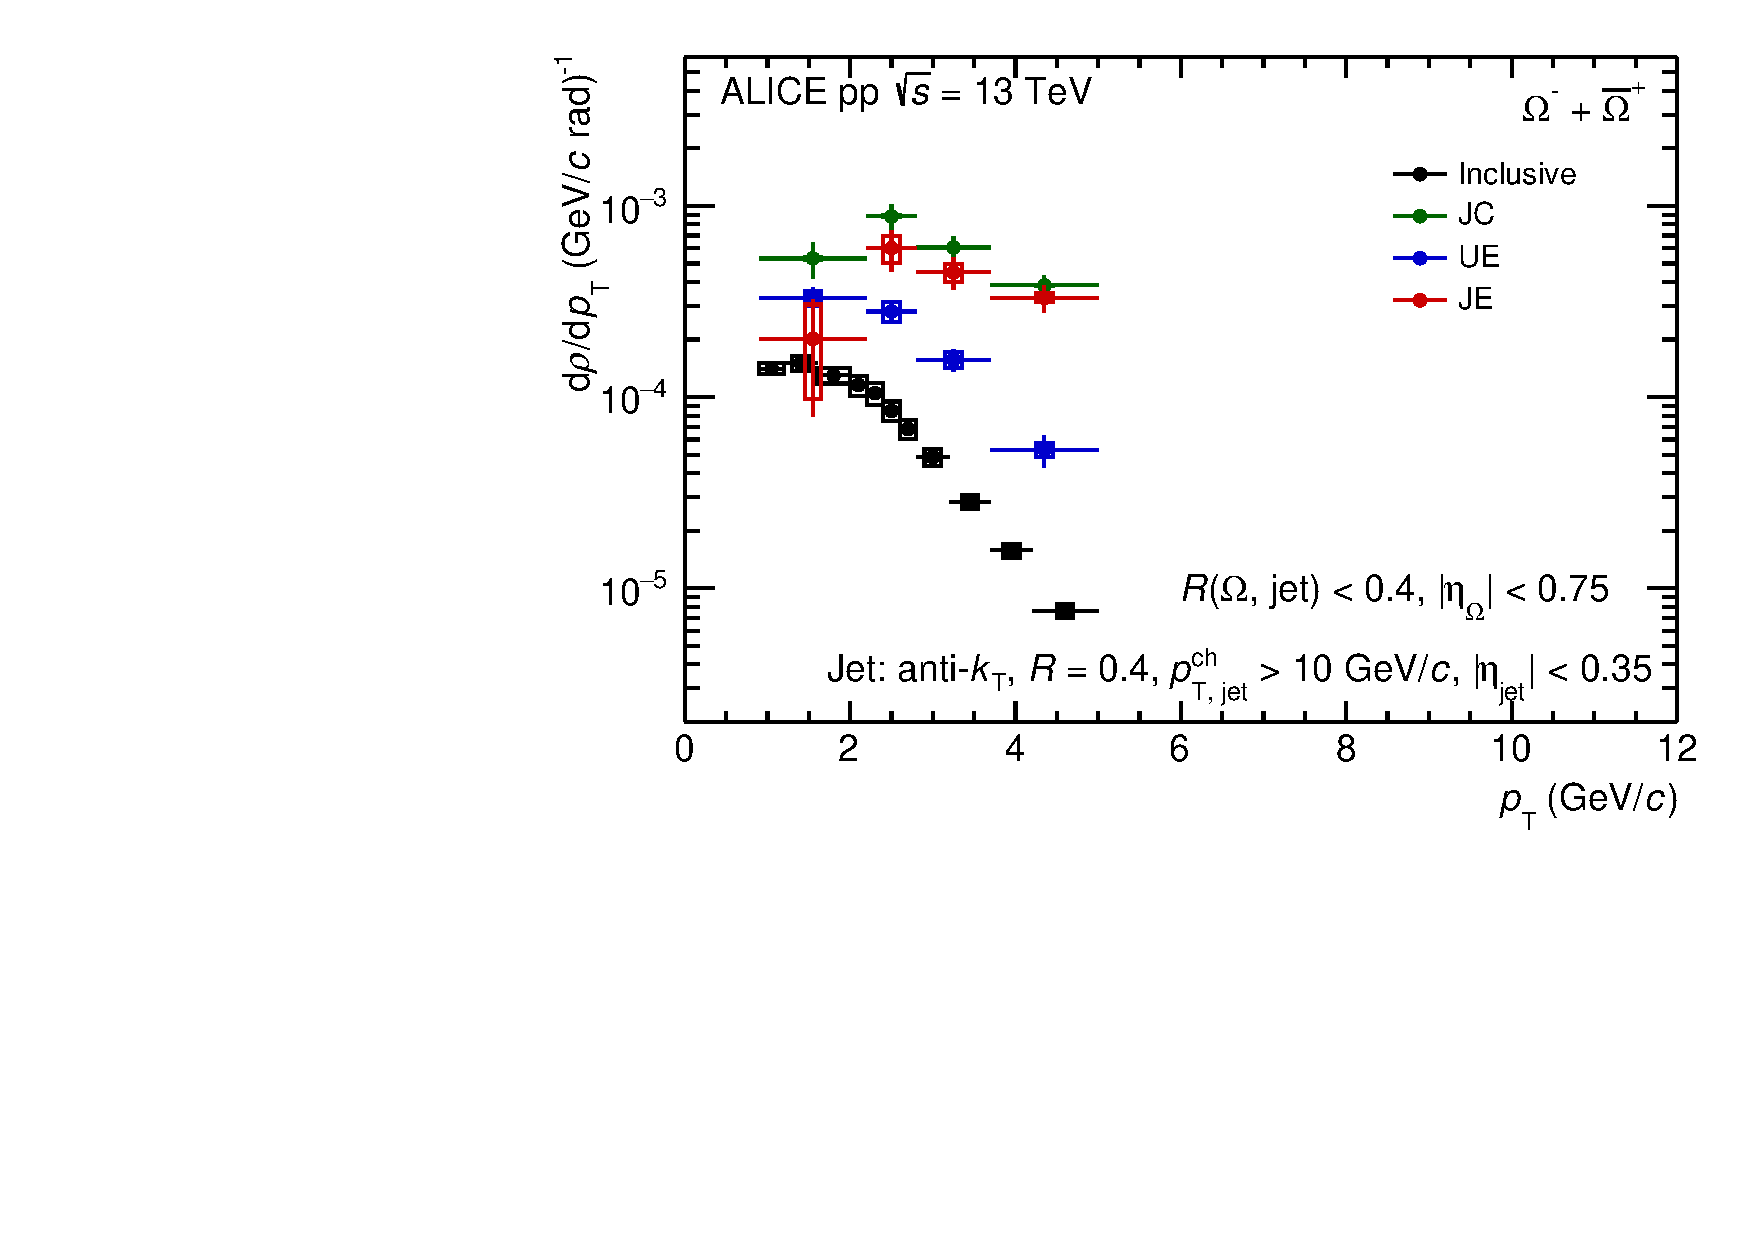
\includegraphics[width=.49\textwidth]{cf04_4}
\end{center}
\caption{$\pT$-differential density of $\kzero$, $\lmb + \almb$, $\X + \Ix$ and $\Om + \Mo$ in \pp collisions at \thirteen. The black points represent particles from minimum bias events, the green points represent particles from the jet cones, the blue points represent particles within a cone perpendicular to the jet, associated with the underlying event and the red points represent the particle from the jet fragmentation.}
\label{fig:ppSpect}
\end{figure}

\begin{figure}[!ht]
\begin{center}
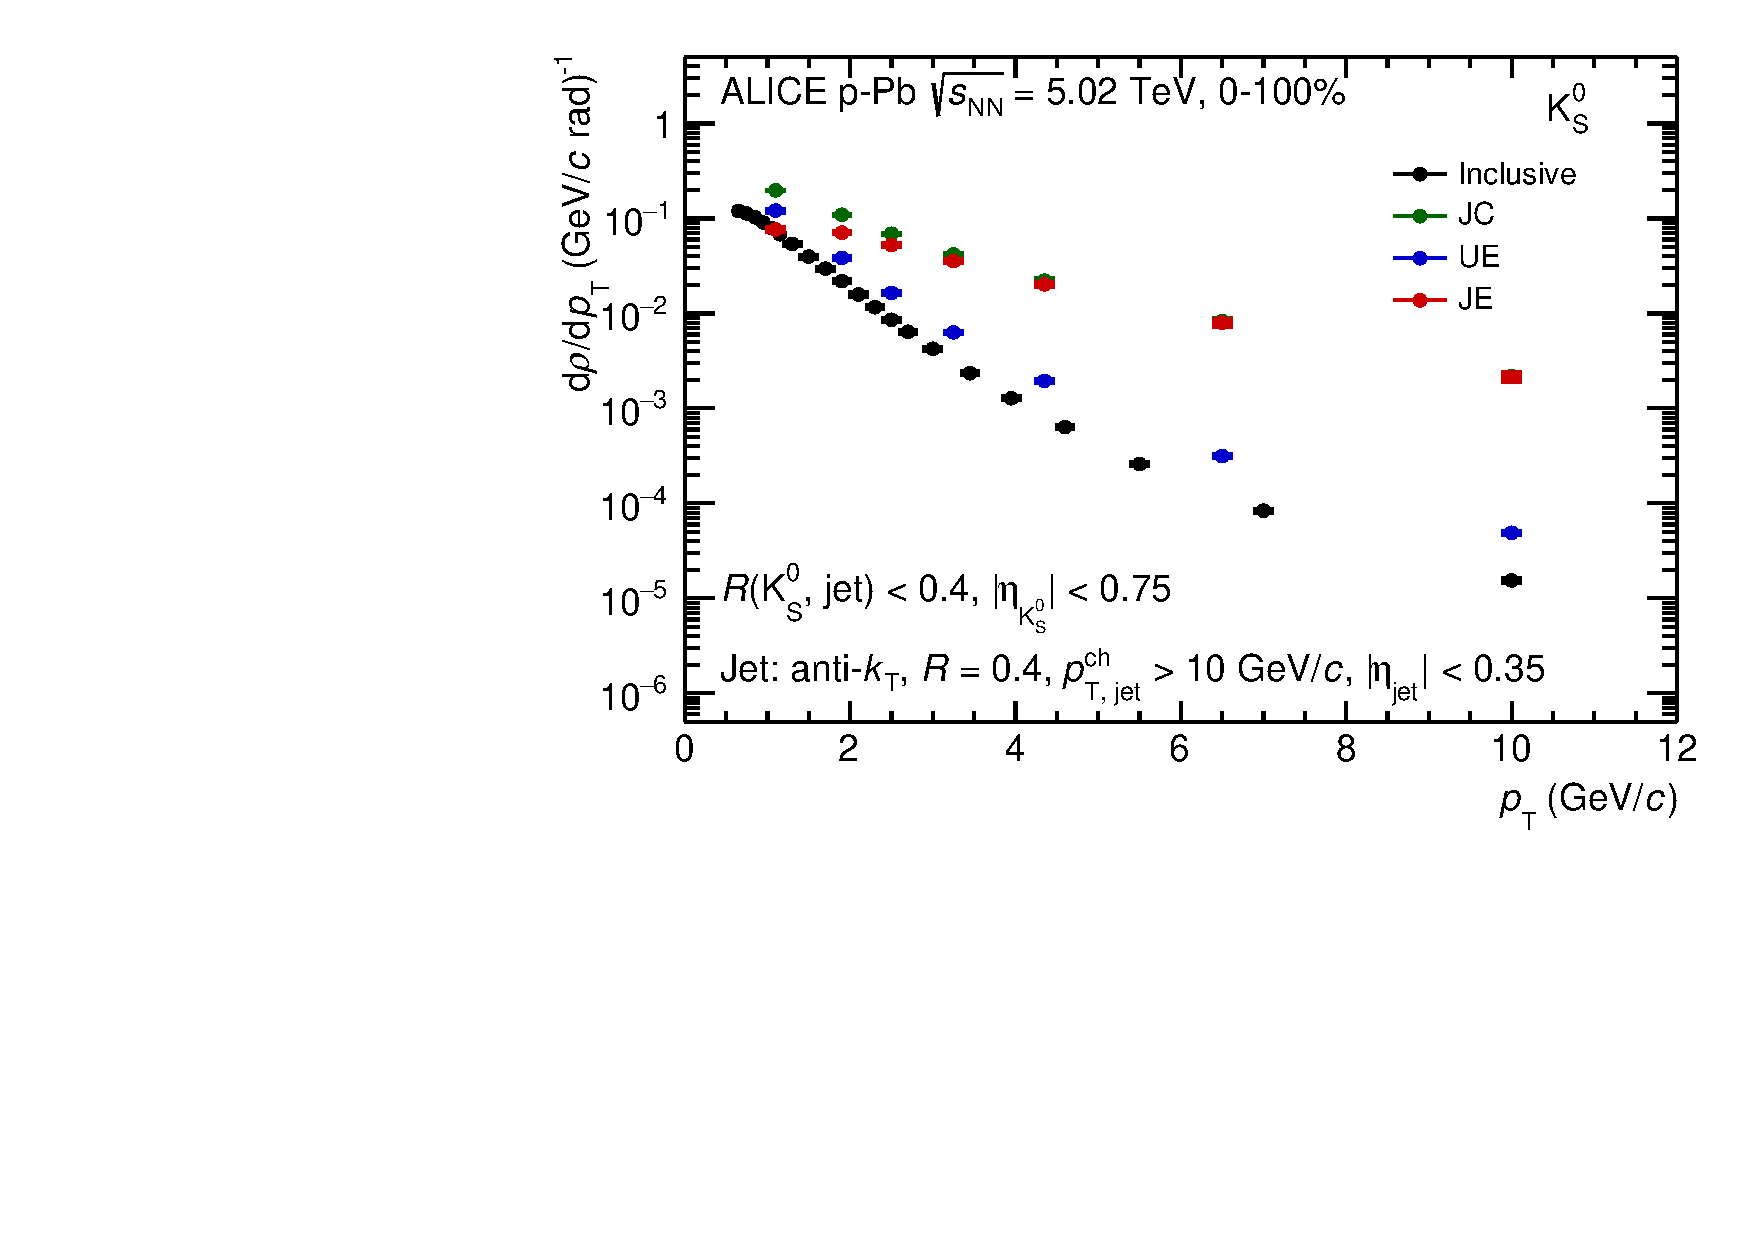
\includegraphics[width=.49\textwidth]{cf05_1}
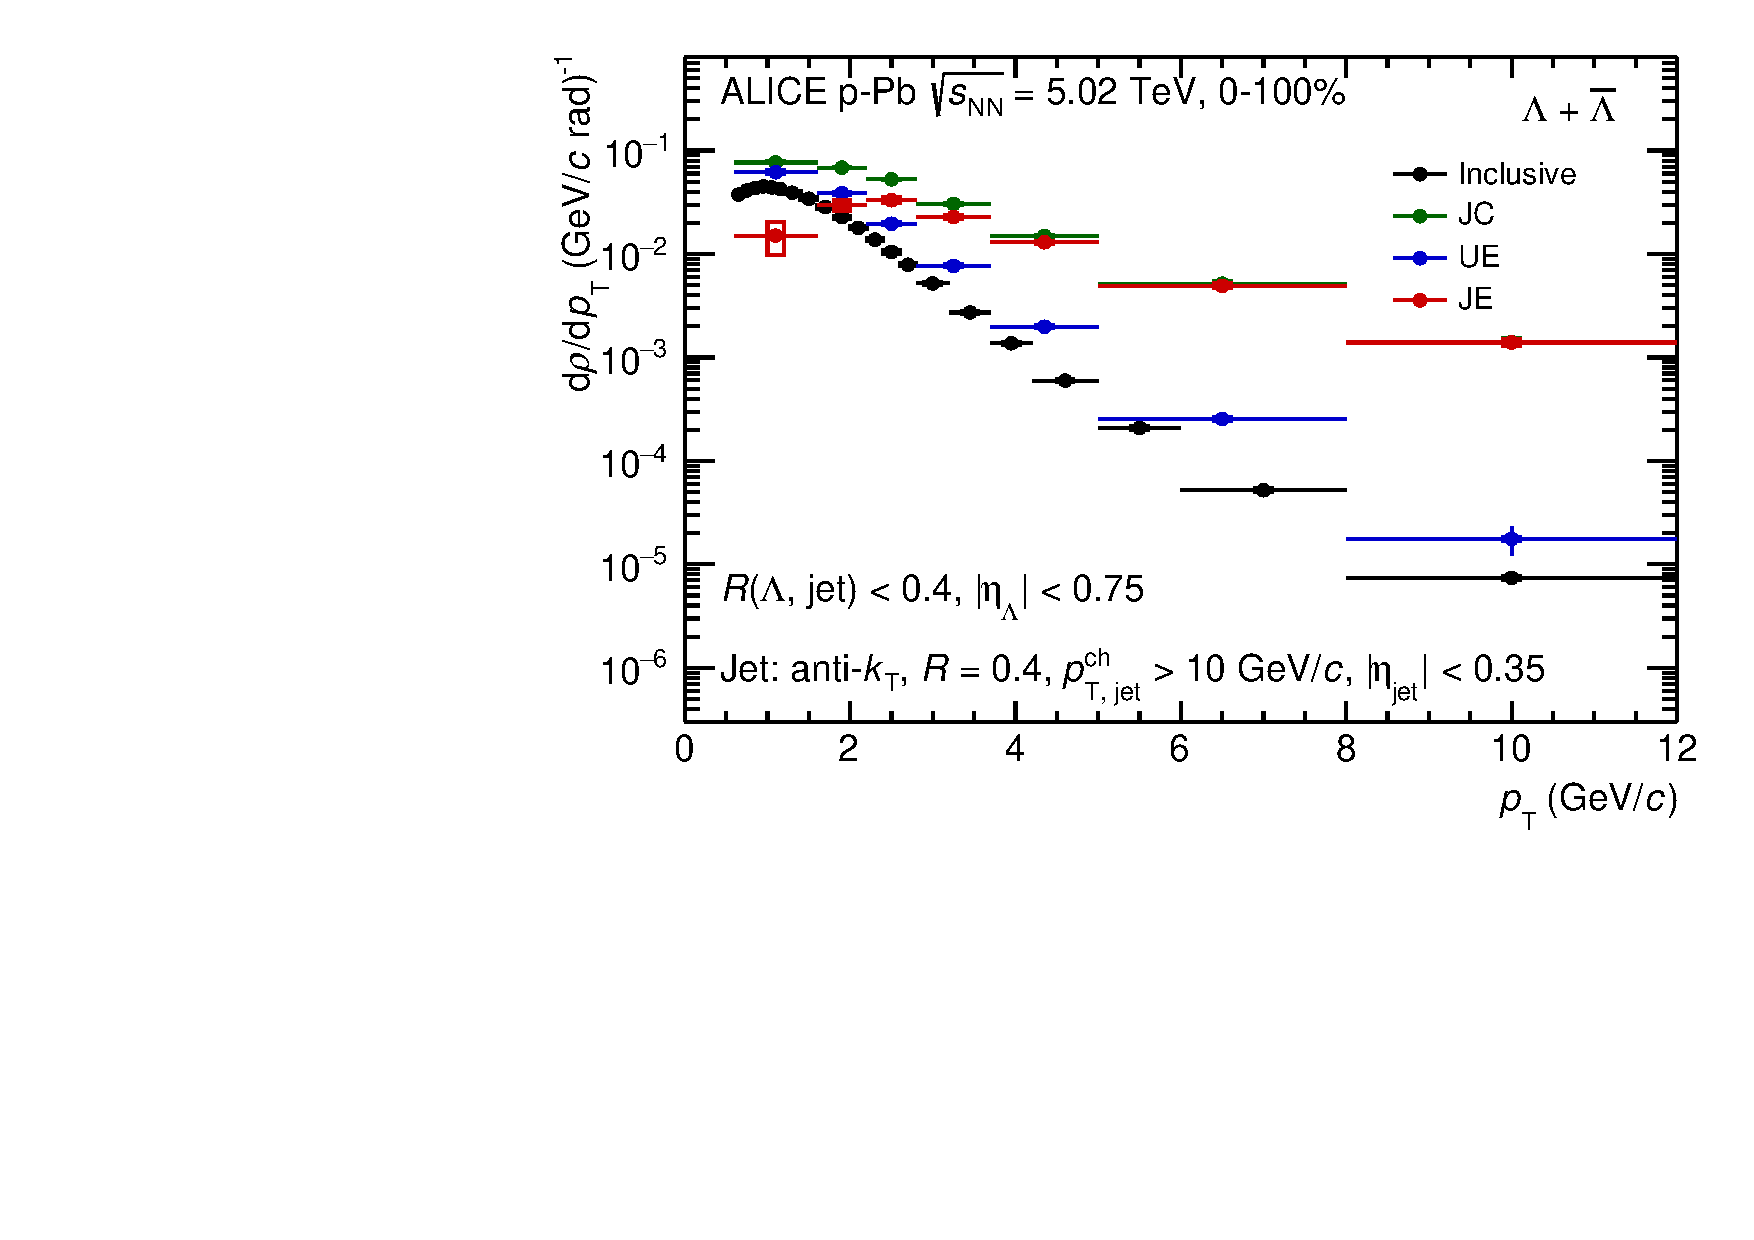
\includegraphics[width=.49\textwidth]{cf05_2}
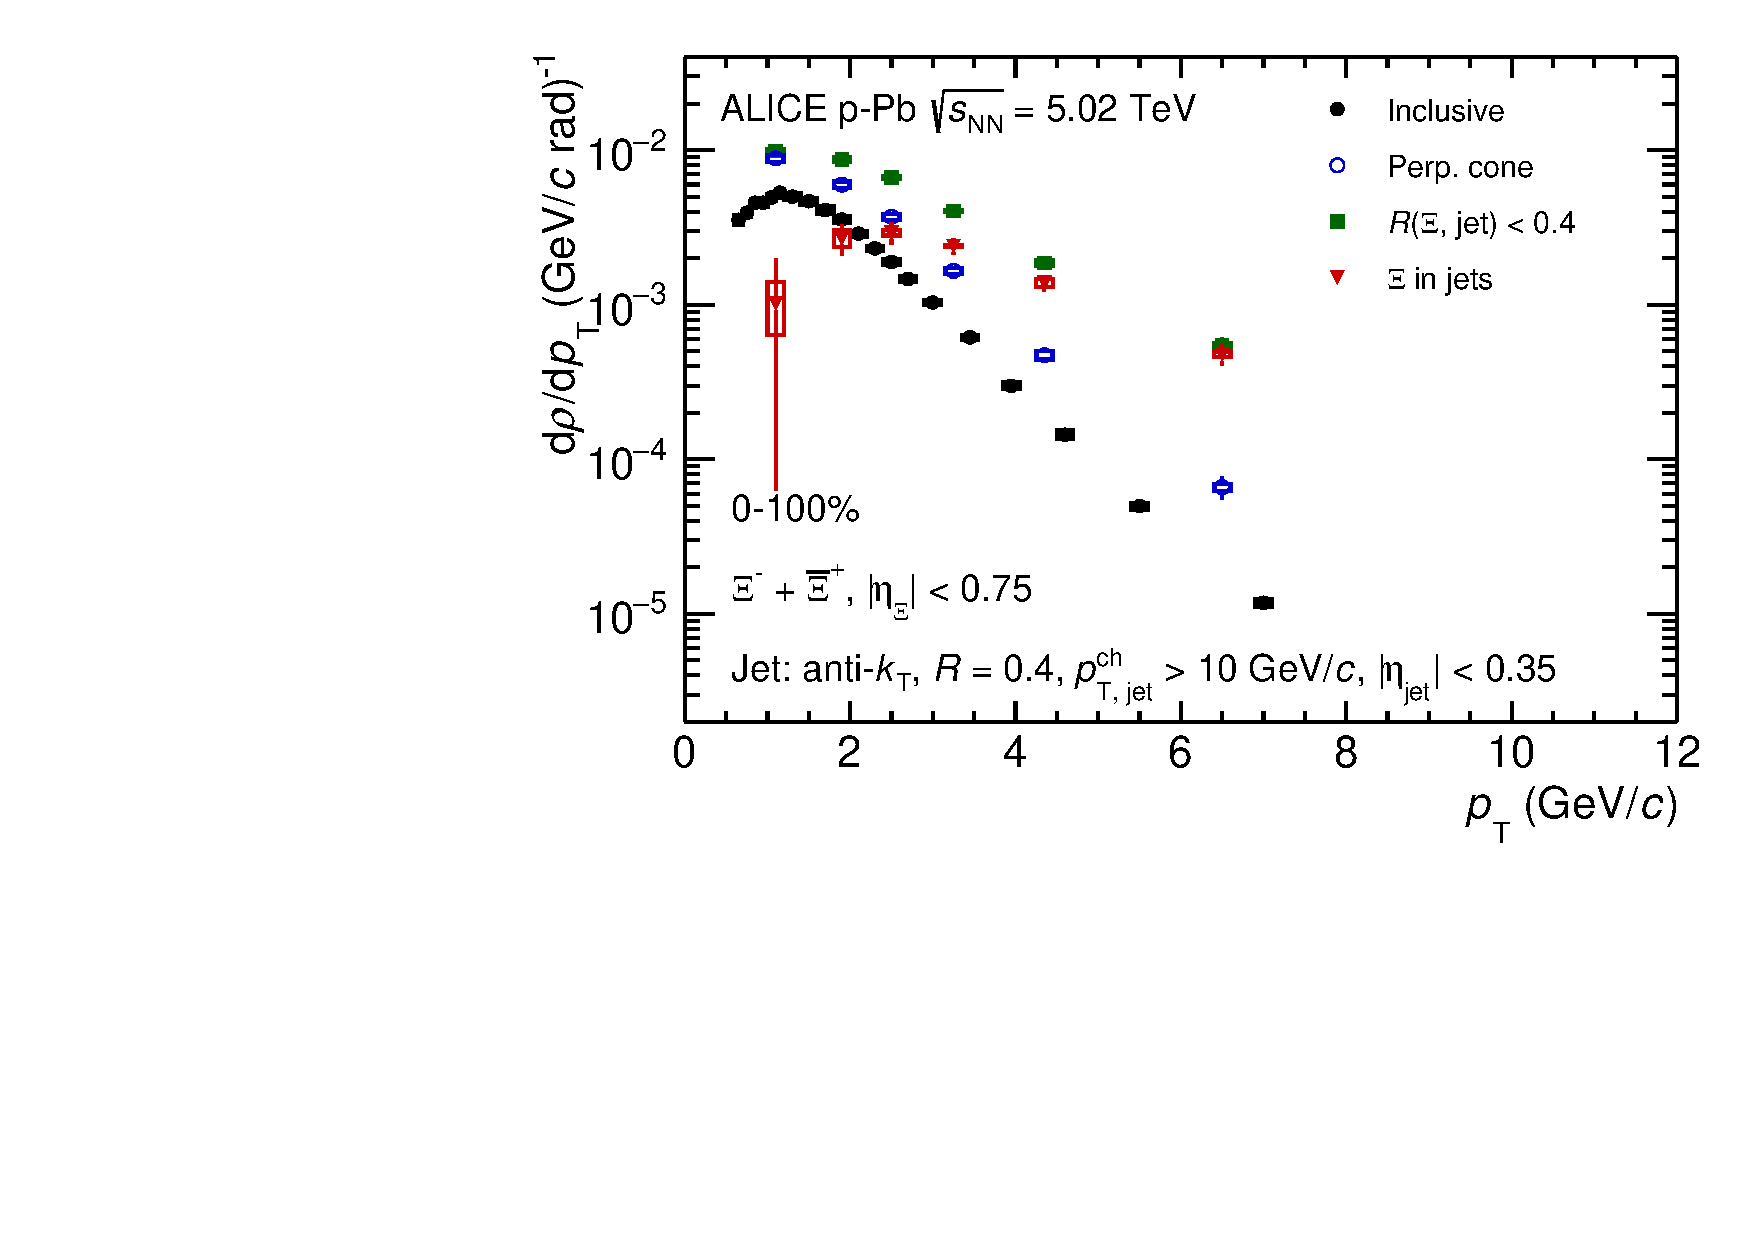
\includegraphics[width=.49\textwidth]{cf05_3}
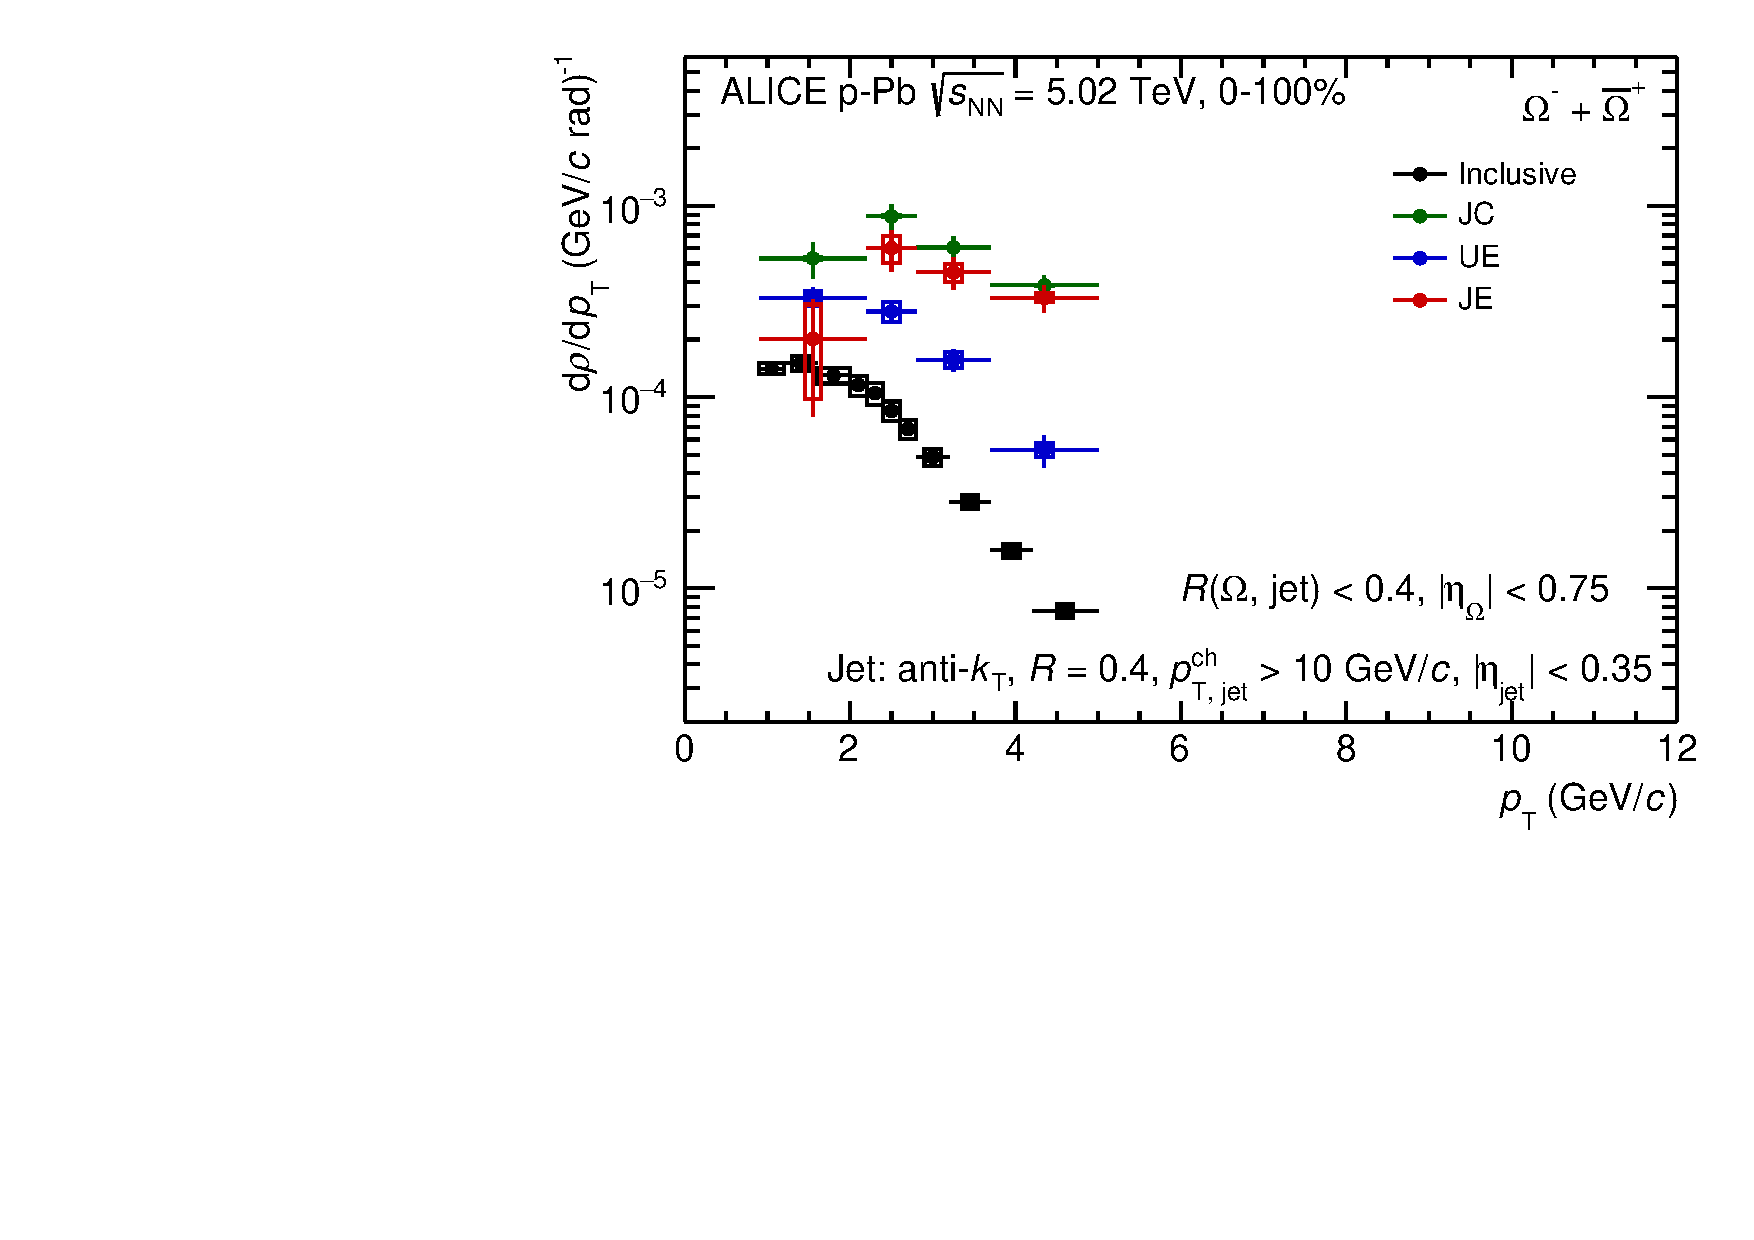
\includegraphics[width=.49\textwidth]{cf05_4}
\end{center}
\caption{$\pT$-differential density of $\kzero$, $\lmb + \almb$, $\X + \Ix$ and $\Om + \Mo$ in 0-100\% in \pPb at \fivenn. The black points represent particles from minimum bias events, the green points represent particles from the jet cones, the blue points represent particles within a cone perpendicular to the jet, associated with the underlying event and the red points represent the particle from the jet fragmentation.}
\label{fig:pPbSpect}
\end{figure}

The fully corrected $\pT$-differential densities ($\dd \rho/ \dd \pT$ defined by Eq.~\ref{eq:normalize}), for \kzero, $\lmb + \almb$, $\X + \Ix$ and $\Om + \Mo$, in \pp and MB \pPb collisions are shown in Fig.~\ref{fig:ppSpect} and \ref{fig:pPbSpect}, respectively.
The $\pT$-differential particle density (d$\rho$/d$\pT$) within charged-particle jets is compared with that of inclusive particles and with perpendicular cone particles.
As expected the $\pT$ dependence of the density of those hadrons within jets,as defined in Eq.~\ref{eq:je}, is considerably less steep than in the case of inclusive particles.
The $\pT$-differential density distribution of inclusive hadrons is lower than that of the PC selection since the latter are obtained from events contain jets with $\pTjch > 10$~\GeVc.
At the high-$\pT$ ($\pT > 4$~\GeVc) region, the density of particle within charged-particle jets is consistent with the one in jet cone (without the underlying event subtraction).
This is consistent with the expectation that the high-$\pT$ particles originate from jet fragmentation.

In the previous studies of ALICE experiment~\cite{ALICE:2015mpp, ALICE:2016dei, ALICE:2013wgn}, the stronger multiplicity dependence of the inclusive $\pT$-differential spectra shapes of heavier particles is observed.
It also a important evidence for the baryon-to-meson ratio enhancement at intermediate-$\pT$.
The $\pT$-differential densities distributions of $\kzero$, $\lmb + \almb$, $\X + \Ix$ and $\Om + \Mo$ particles within jet are shown in Fig.~\ref{fig:pPbSpectwCent} for different charged-particle multiplicity bins.
The bottom panels depict the ratio to the minimum bias (0-100\%) $\pT$ distribution.
For the $\Om + \Mo$ in jet density, only the minimum bias distribution is shown.
These spectra are compared to the particles in charged-particle jets with PYTHIA 8 simulation with Monash tune.
The PYTHIA 8 can describe the $\kzero$ and $\lmb + \almb$ well, but not for the $\X + \Ix$ and $\Om + \Mo$.
In Fig.~\ref{fig:pPbSpectwCent}, the $\kzero$, $\lmb + \almb$ and $\X + \Ix$  particle $\pT$ spectra do not show any dependent on the charged-particle multiplicity which observed in that of inclusive particles~\cite{ALICE:2015mpp, ALICE:2016dei, ALICE:2013wgn}.
Then the particle associated with jet fragmentation process may not contribute on the baryon-to-meson ratio enhancement in high multiplicity INEL events with respect to that in lower multiplicity events in small collision systems.

\begin{figure}[!ht]
\begin{center}
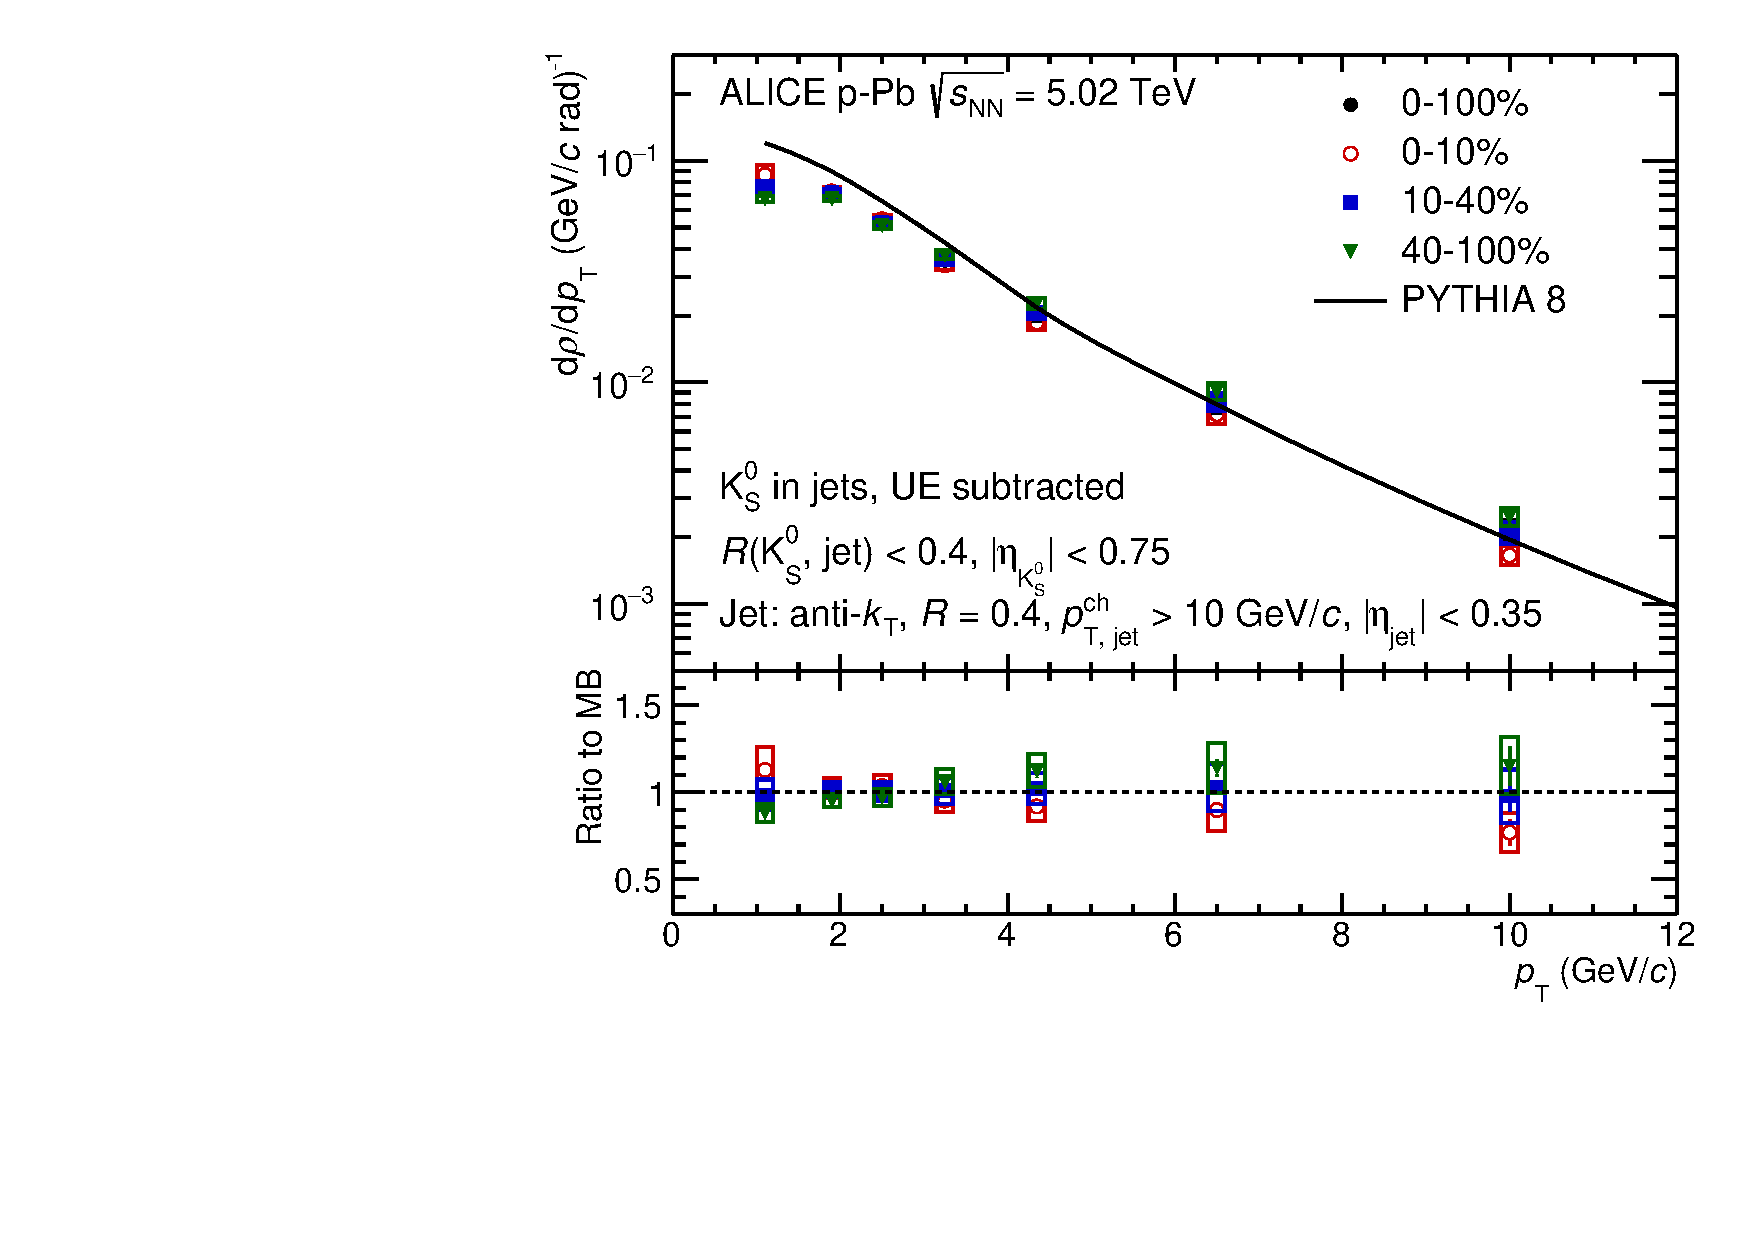
\includegraphics[width=.49\textwidth]{cf06_4}
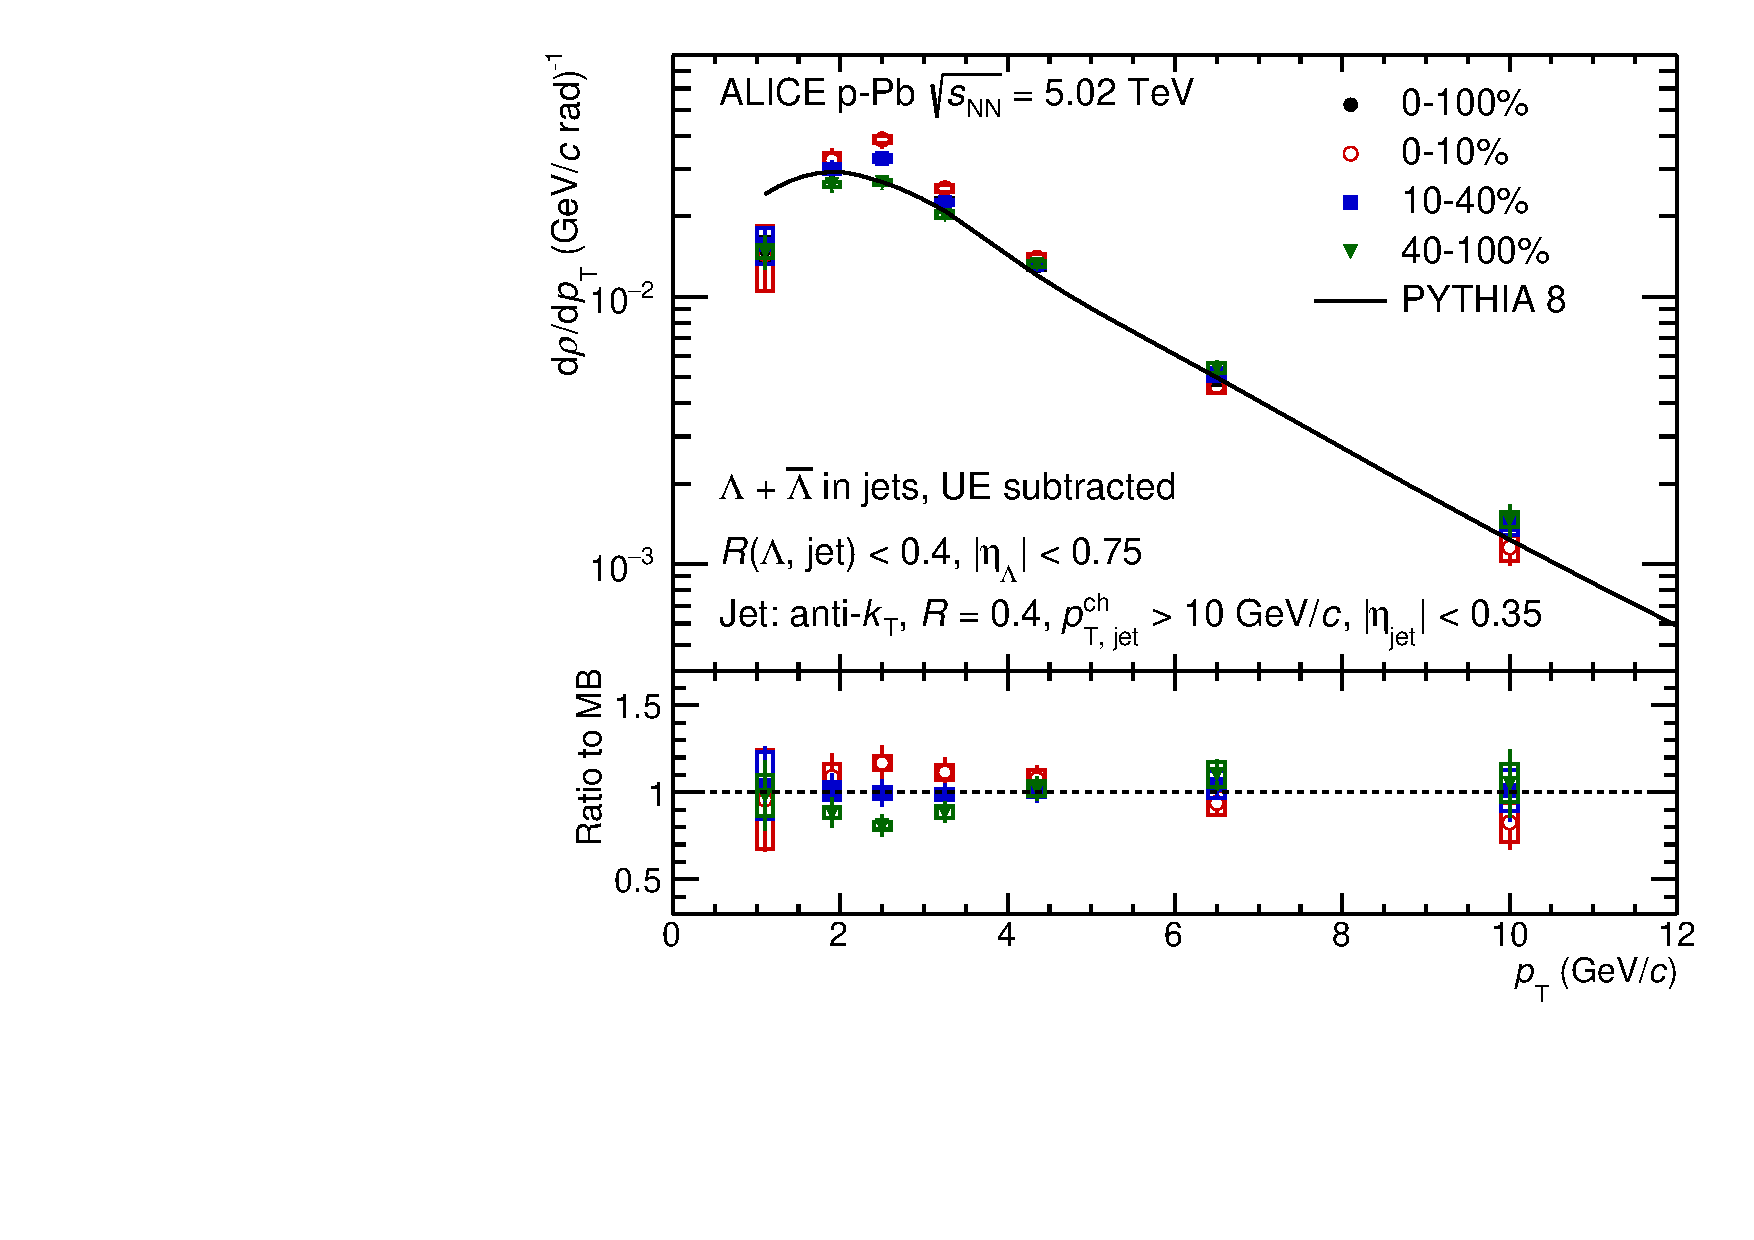
\includegraphics[width=.49\textwidth]{cf06_5}
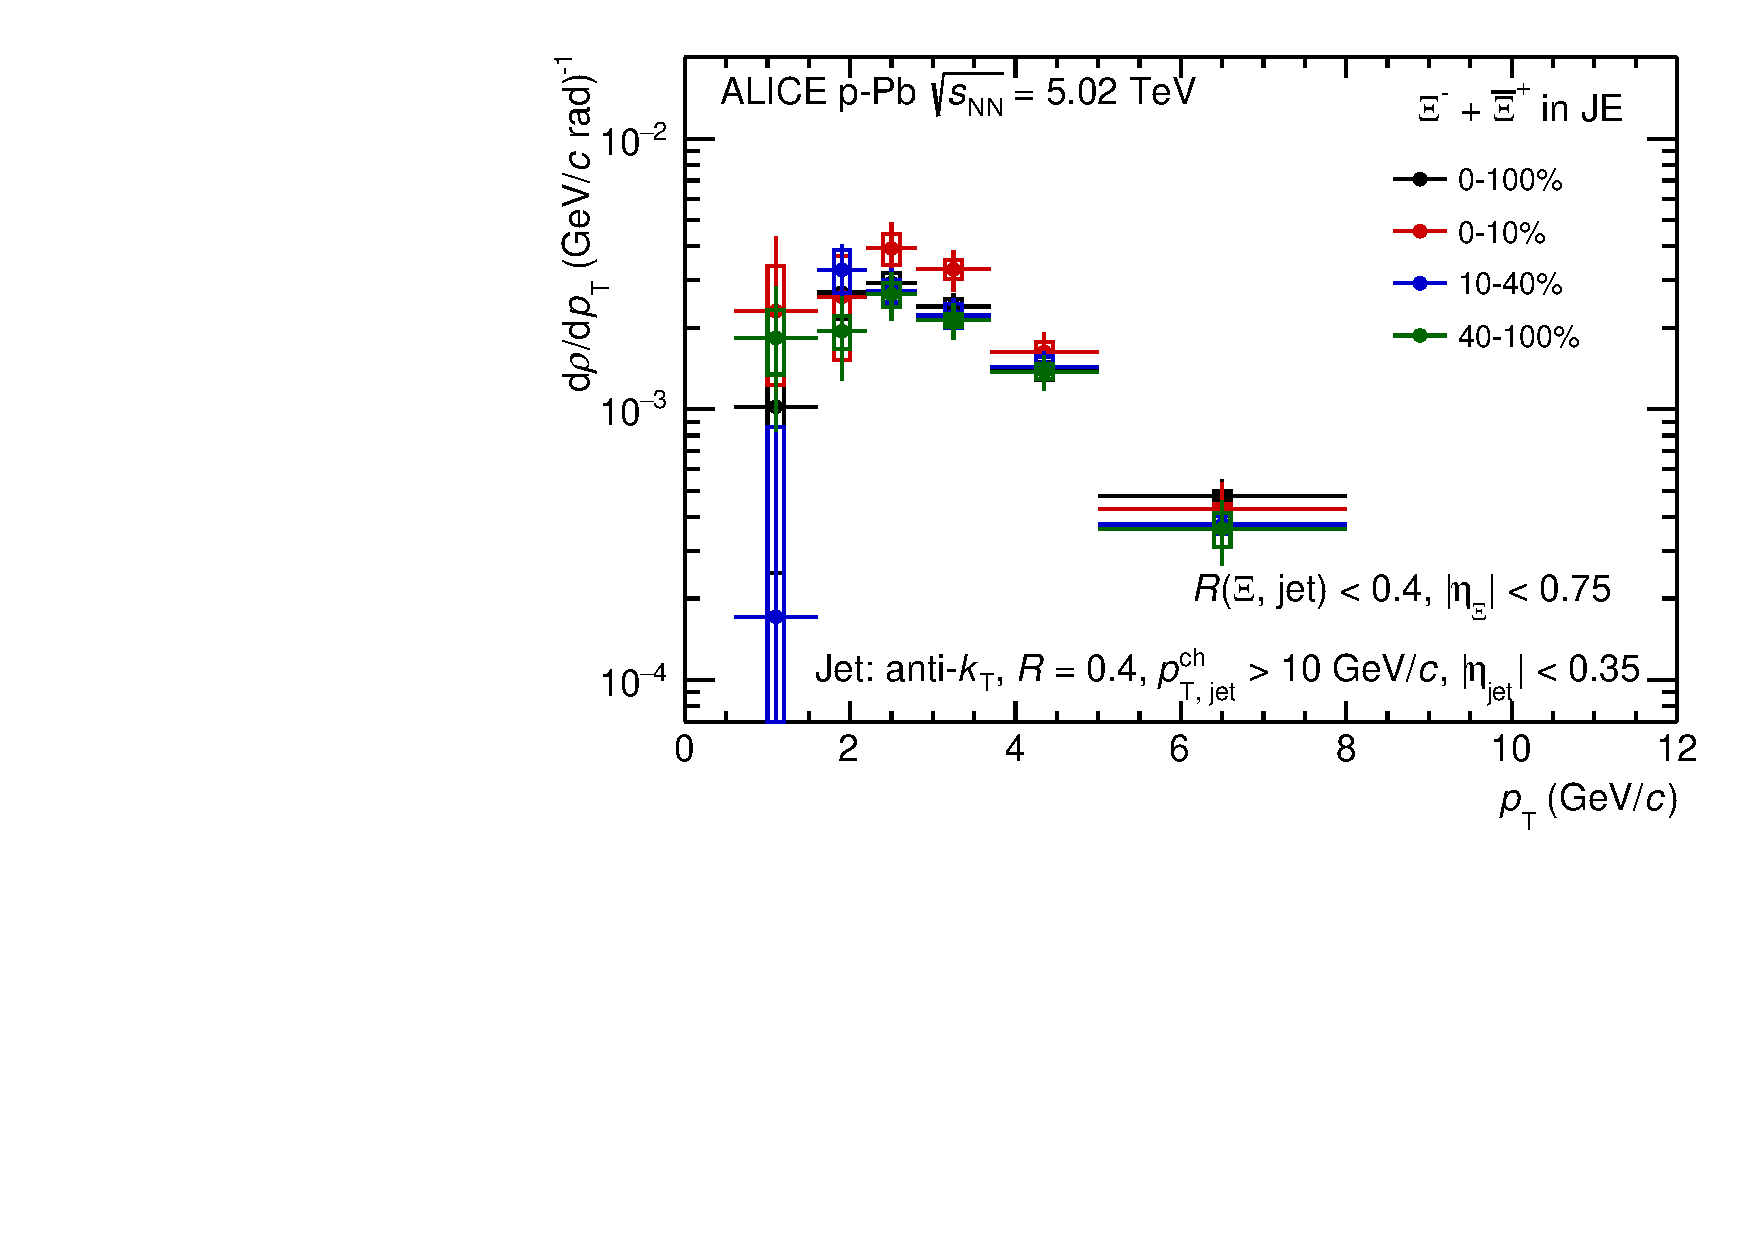
\includegraphics[width=.49\textwidth]{cf06_6}
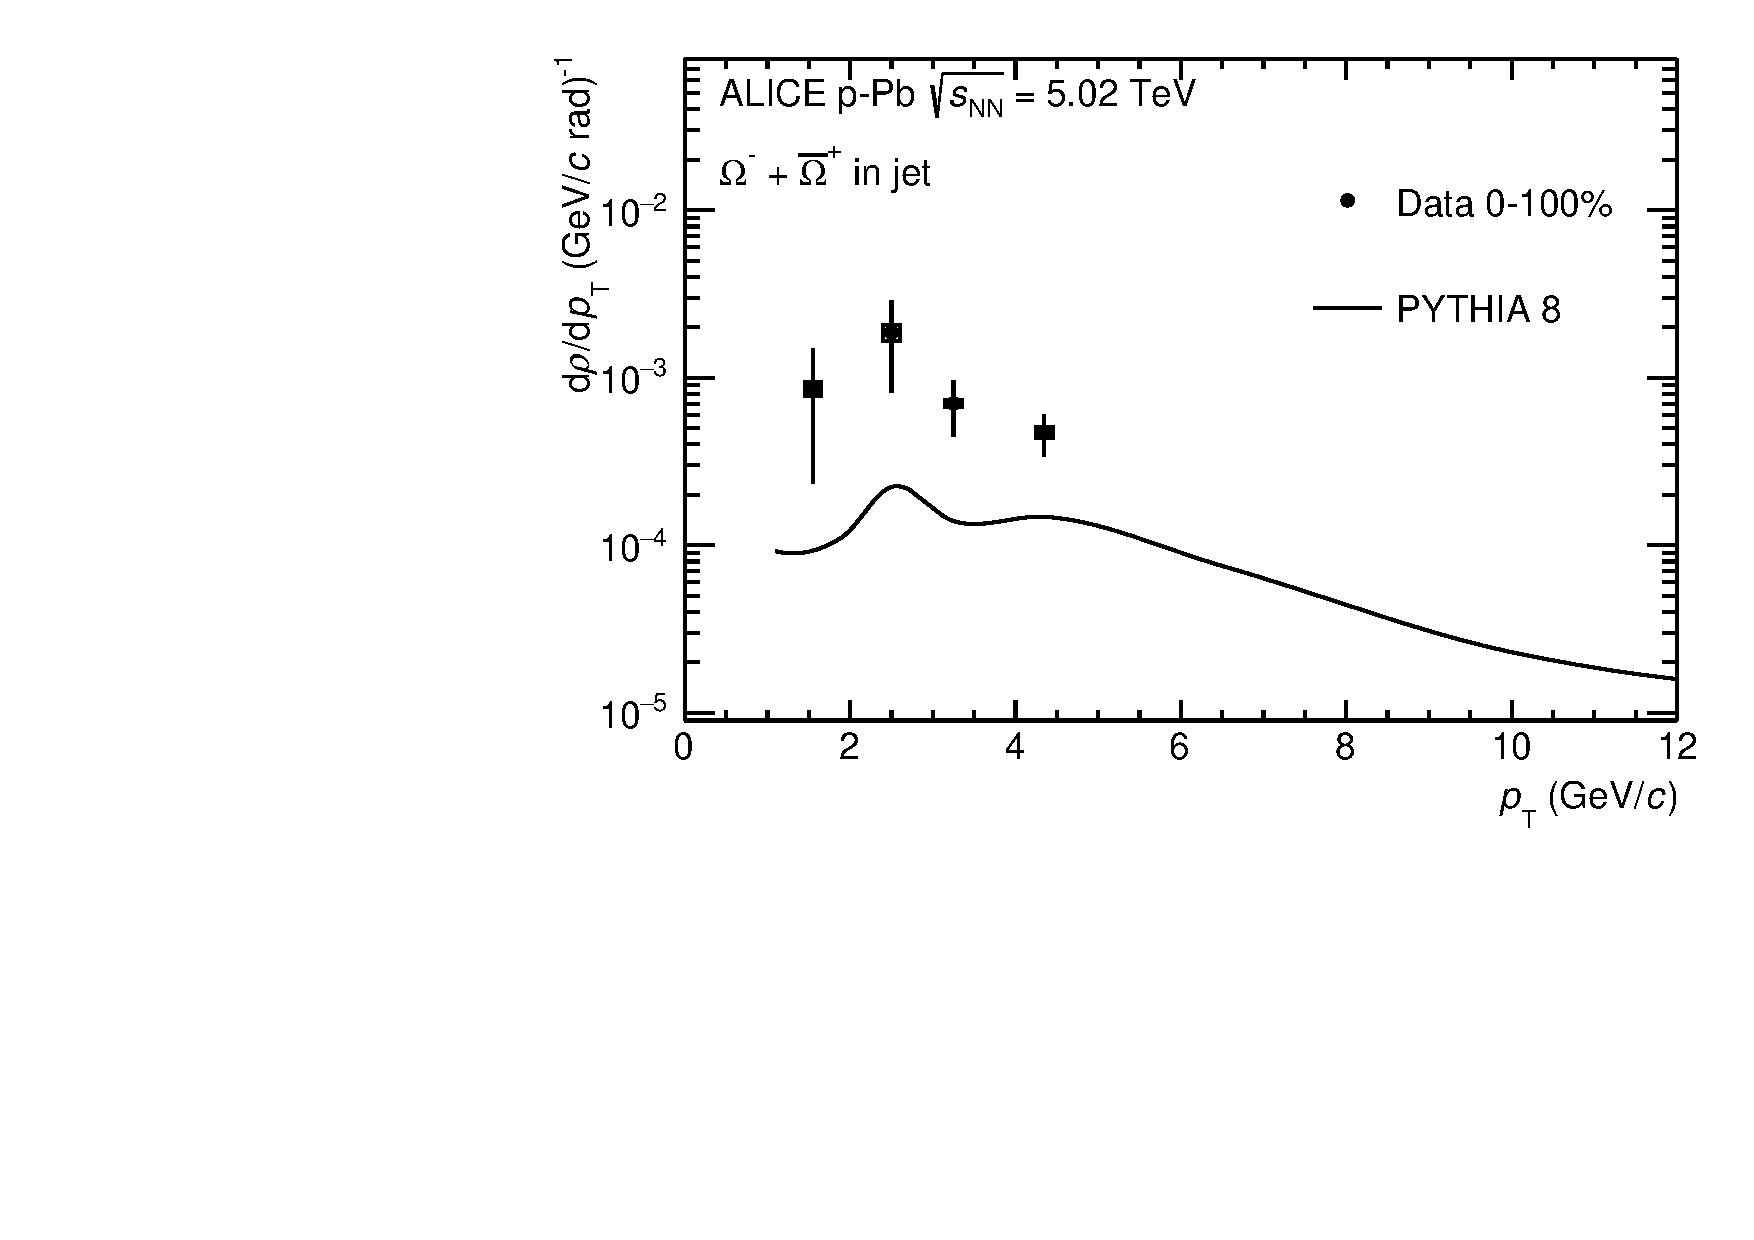
\includegraphics[width=.49\textwidth]{cf06_7}
\end{center}
\caption{$\pT$-differential density of $\kzero$, $\lmb + \almb$, $\X + \Ix$ and $\Om + \Mo$ (0-100\% only) particles within jets in different V0A event multiplicity classes in \pPb collisions at \fivenn. The different centrality classes are depicted with different color. In the bottom panels ratios of multiplicity dependent spectra to minimum bias are shown. The systematic uncertainties on the ratios are obtained by considering only contributions uncorrelated across multiplicity.
The dashed curves represent PYTHIA 8 simulations to the measured spectra.}
\label{fig:pPbSpectwCent}
\end{figure}

\clearpage
\subsection{Baryon-to-meson and baryon-to-baryon ratios}
\label{subsec:ParRatios}
The $(\lmb + \almb)/2\kzero$, $(\X + \Ix)/2\kzero$ and $(\Om + \Mo)/2\kzero$ baryon-to-meson ratios and $(\X + \Ix)/(\lmb + \almb)$, $(\Om + \Mo)/(\lmb + \almb)$ and $(\Om + \Mo)/(\X + \Ix)$ baryon-to-baryon ratios can be obtained by dividing the normalized density distributions.
This ratios are investigated as a function of $\pT$ for several selections which are introduced in Sec.~\ref{sec:ParJetMatch} in \pp and \pPb collisions.
As can be seen in Fig.~\ref{fig:ppRatio} (\pp collisions at \thirteen) and Fig.~\ref{fig:pPbRatio} (\pPb collisions at \fivenn, 0-100\%), the inclusive and the PC particle ratio distributions manifest an enhancement at $\pT \sim 3 - 4 $~\GeVc.
The measurement of the inclusive case differs from that in Ref.~\cite{ALICE:2015mpp, ALICE:2016dei, ALICE:2013wgn} as the region $|\eta_{\rm lab}| < 0.75$ is used here instead of the rapidity region in centre-of-mass frame $0 < y_{\rm CMS} < 0.5$.
The measurement is ortherwise consistent with them.
The ratios within charged-particle jets are significantly lower than those for the inclusive and UE case at low and intermediate $\pT$.
Also the ratios in jet are approximately independent of $\pT$ beyond 2~\GeVc.
This suggests that the ratios of baryon-to-meson and baryon-to-baryon enhancement at intermediate $\pT$ is not driven by the jet fragmentation.

\begin{figure}[!ht]
\begin{center}
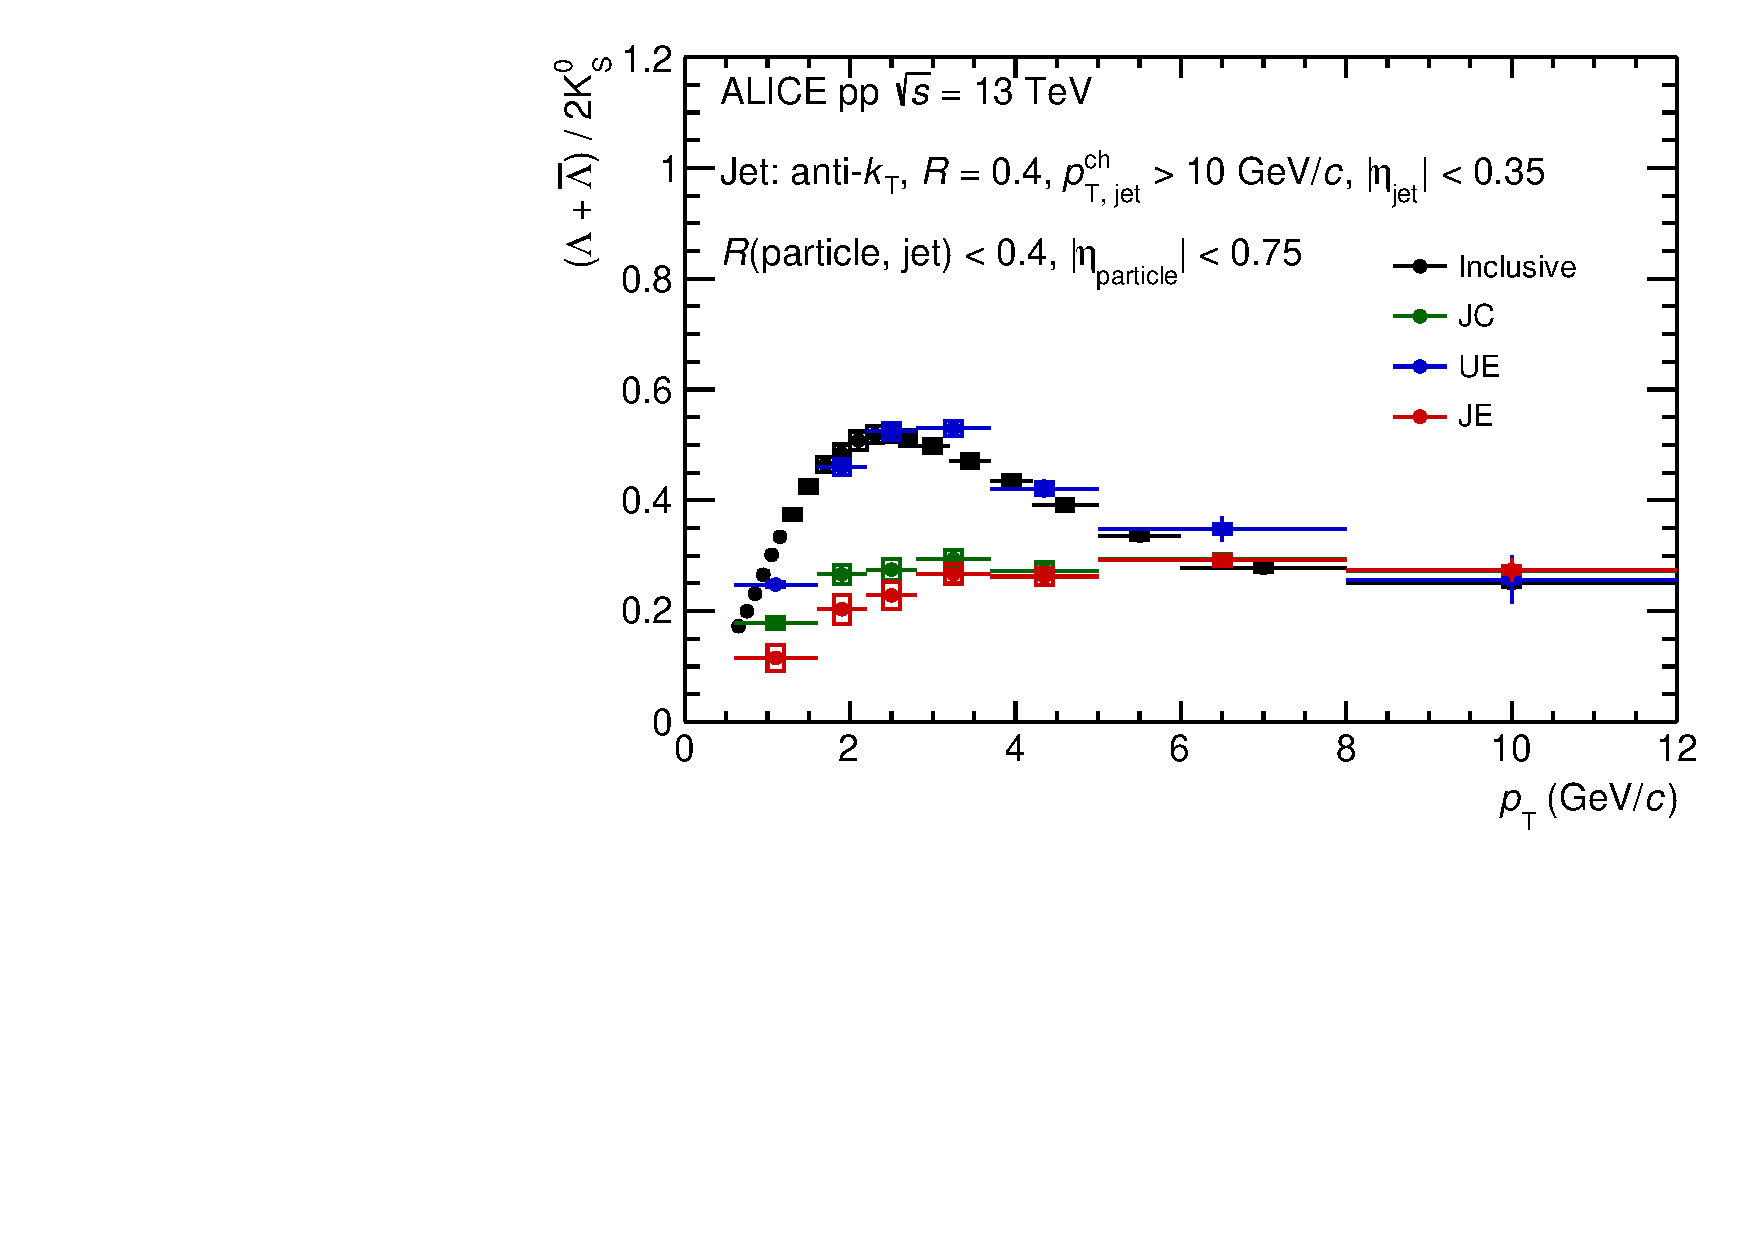
\includegraphics[width=.49\textwidth]{cf07_1}
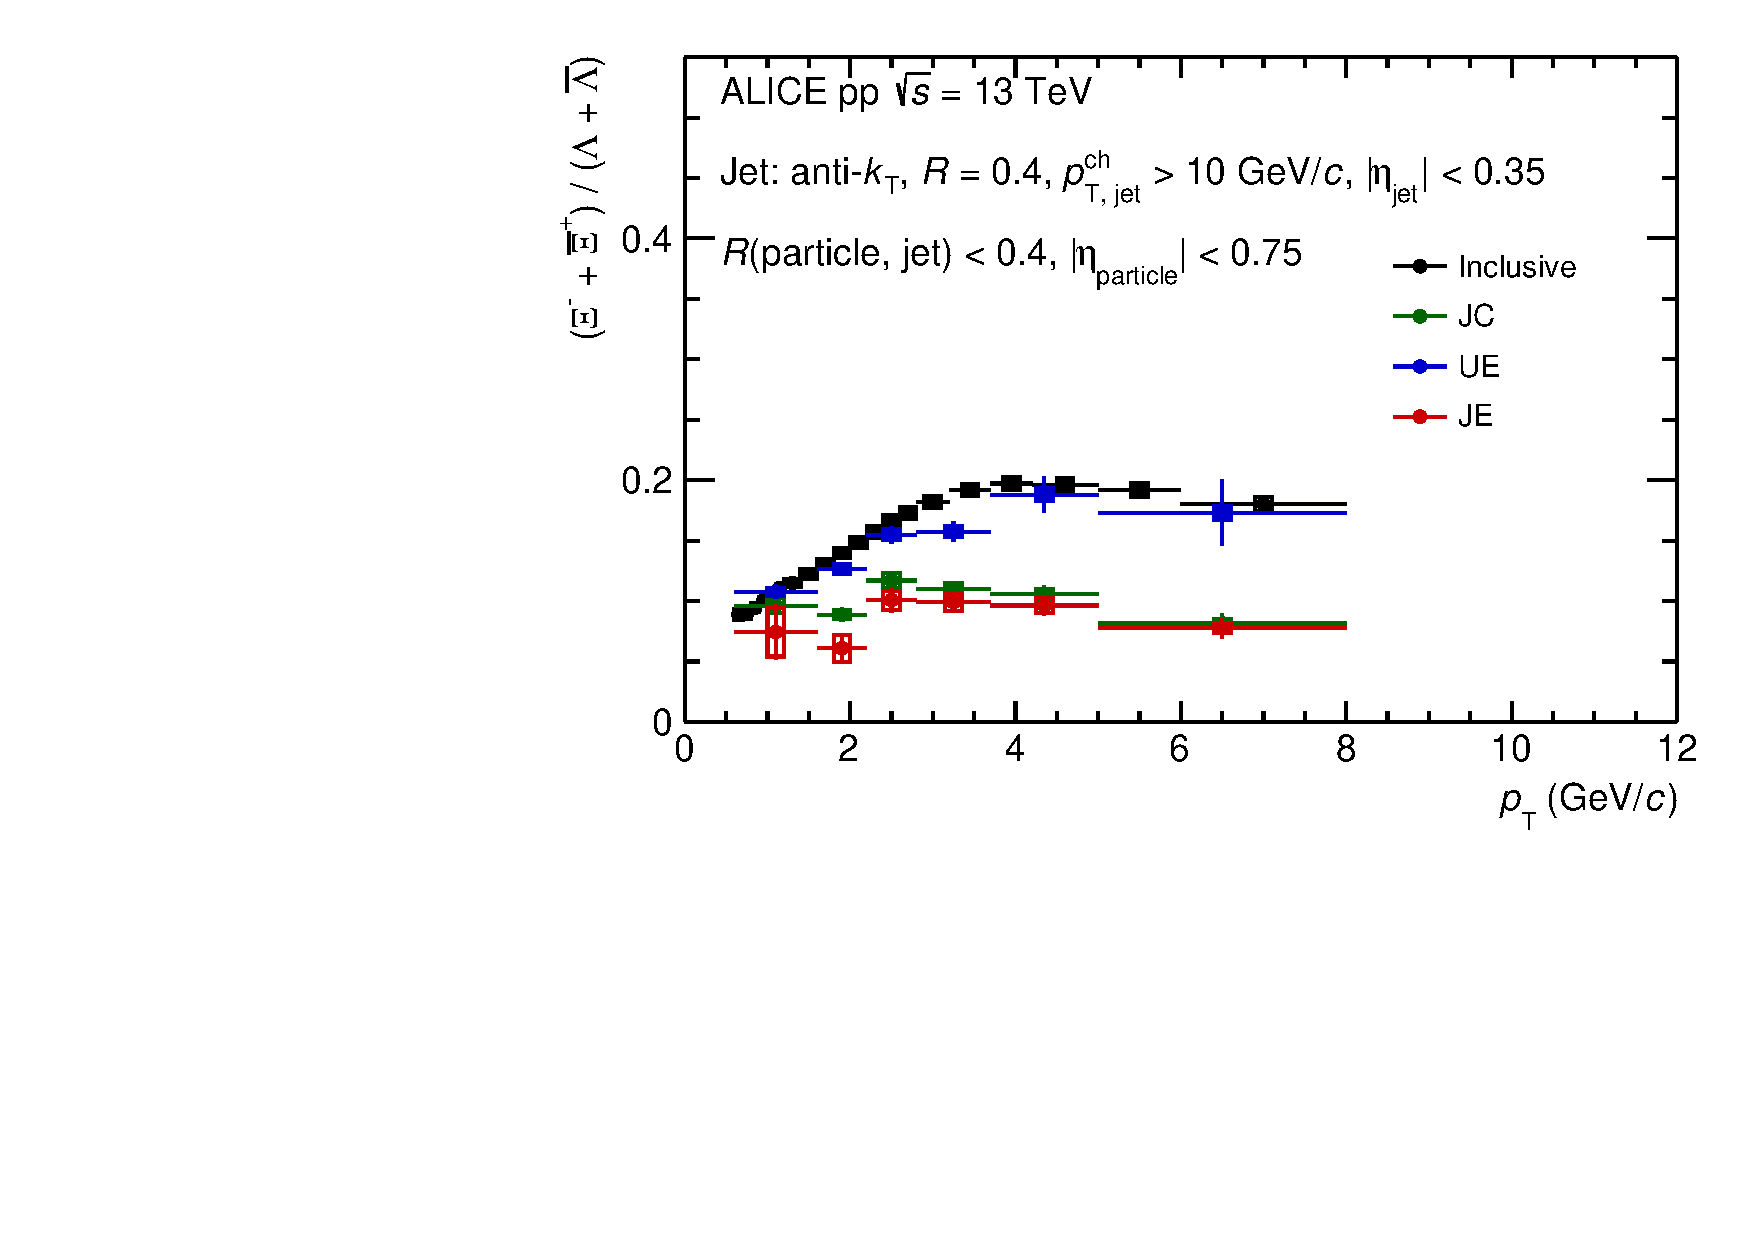
\includegraphics[width=.49\textwidth]{cf07_4}
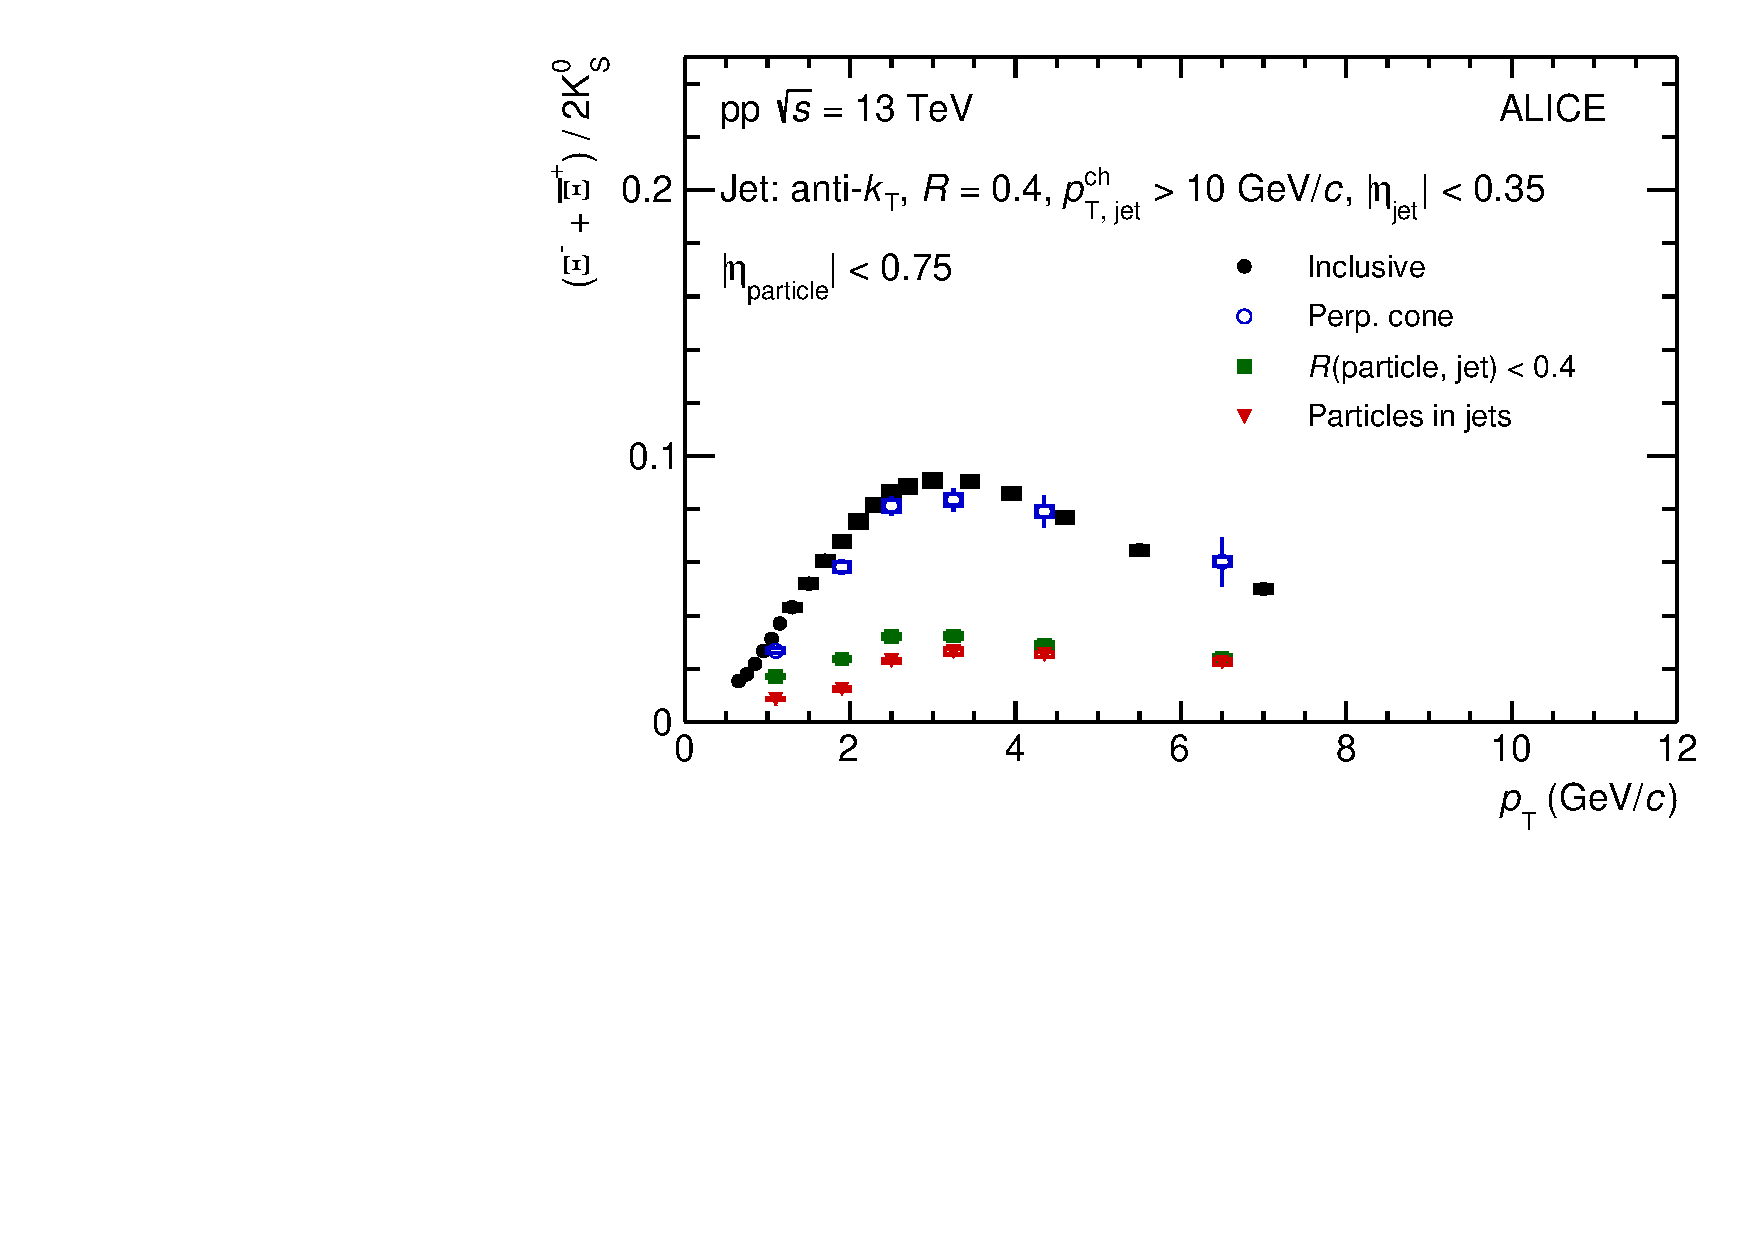
\includegraphics[width=.49\textwidth]{cf07_2}
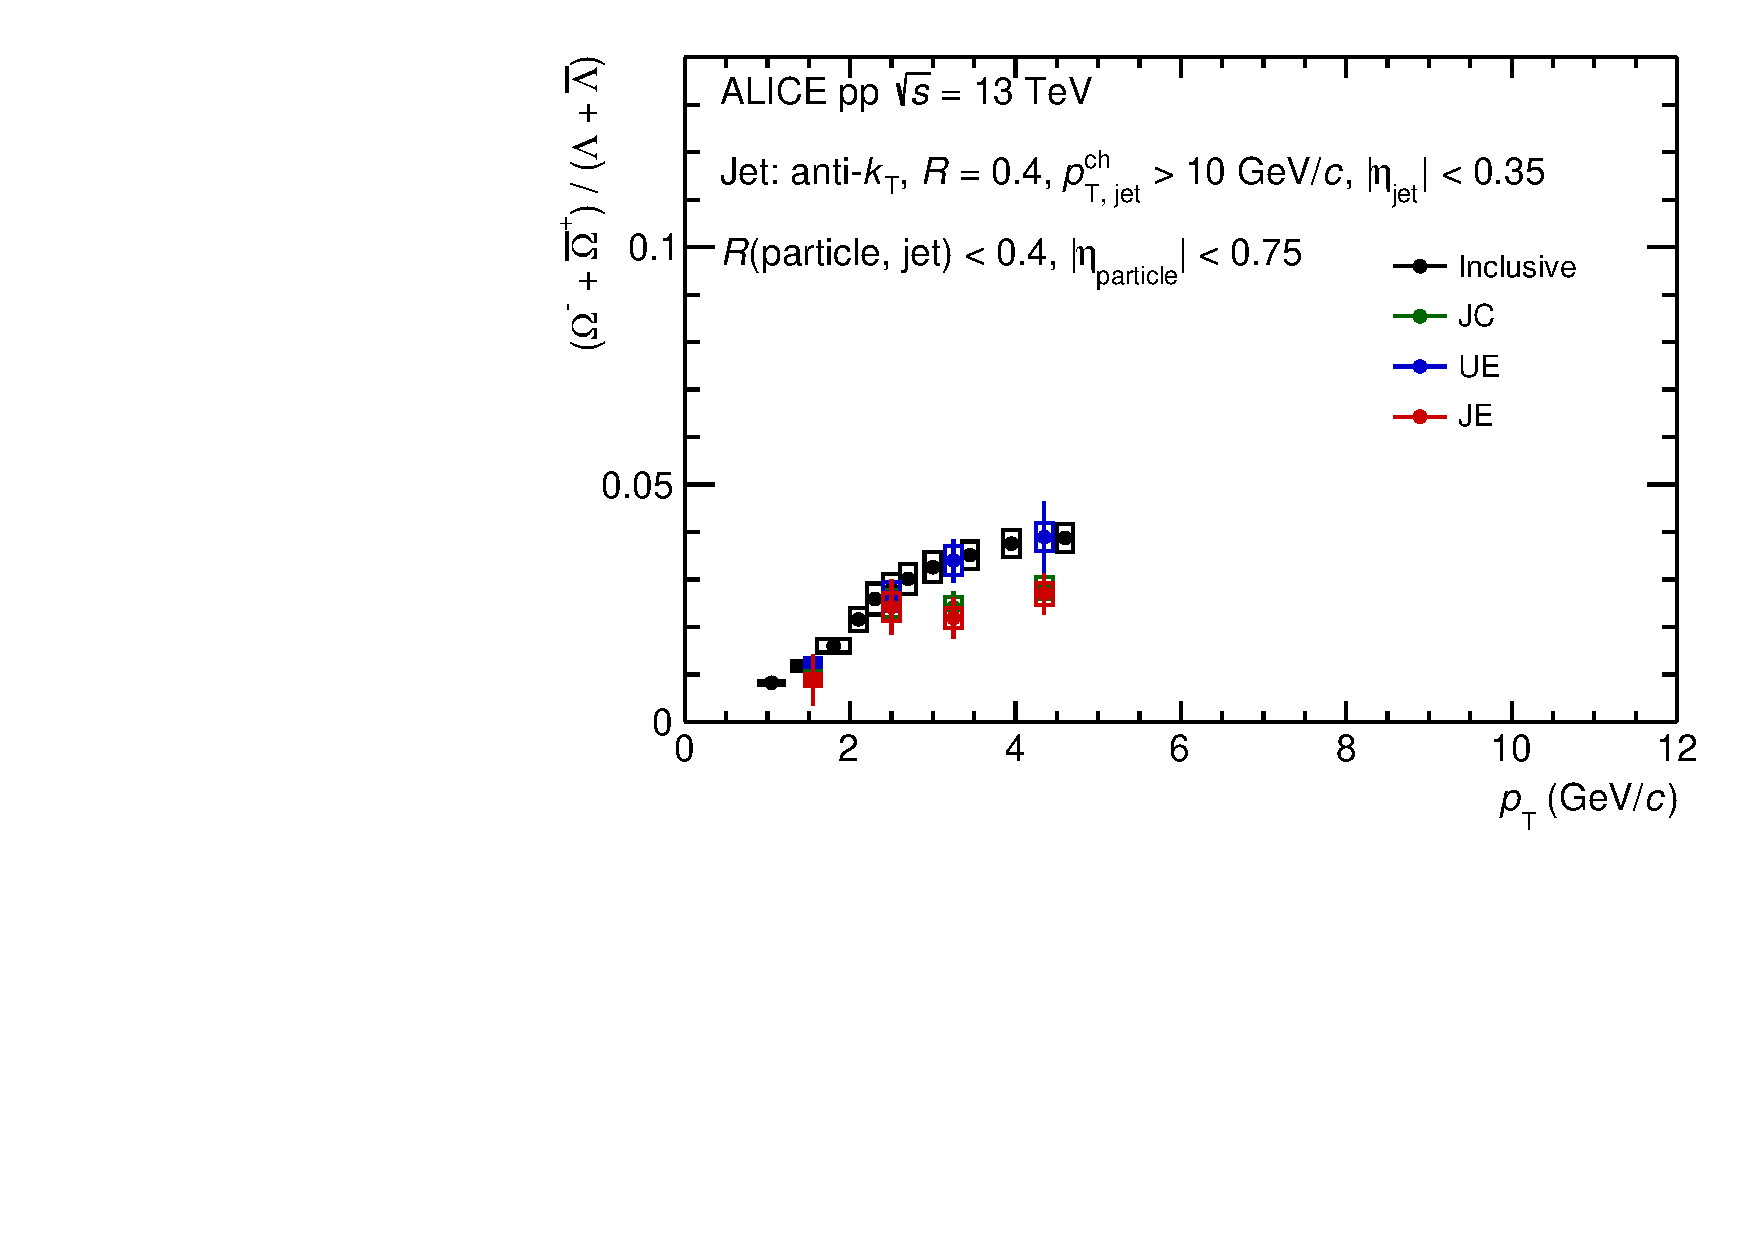
\includegraphics[width=.49\textwidth]{cf07_5}
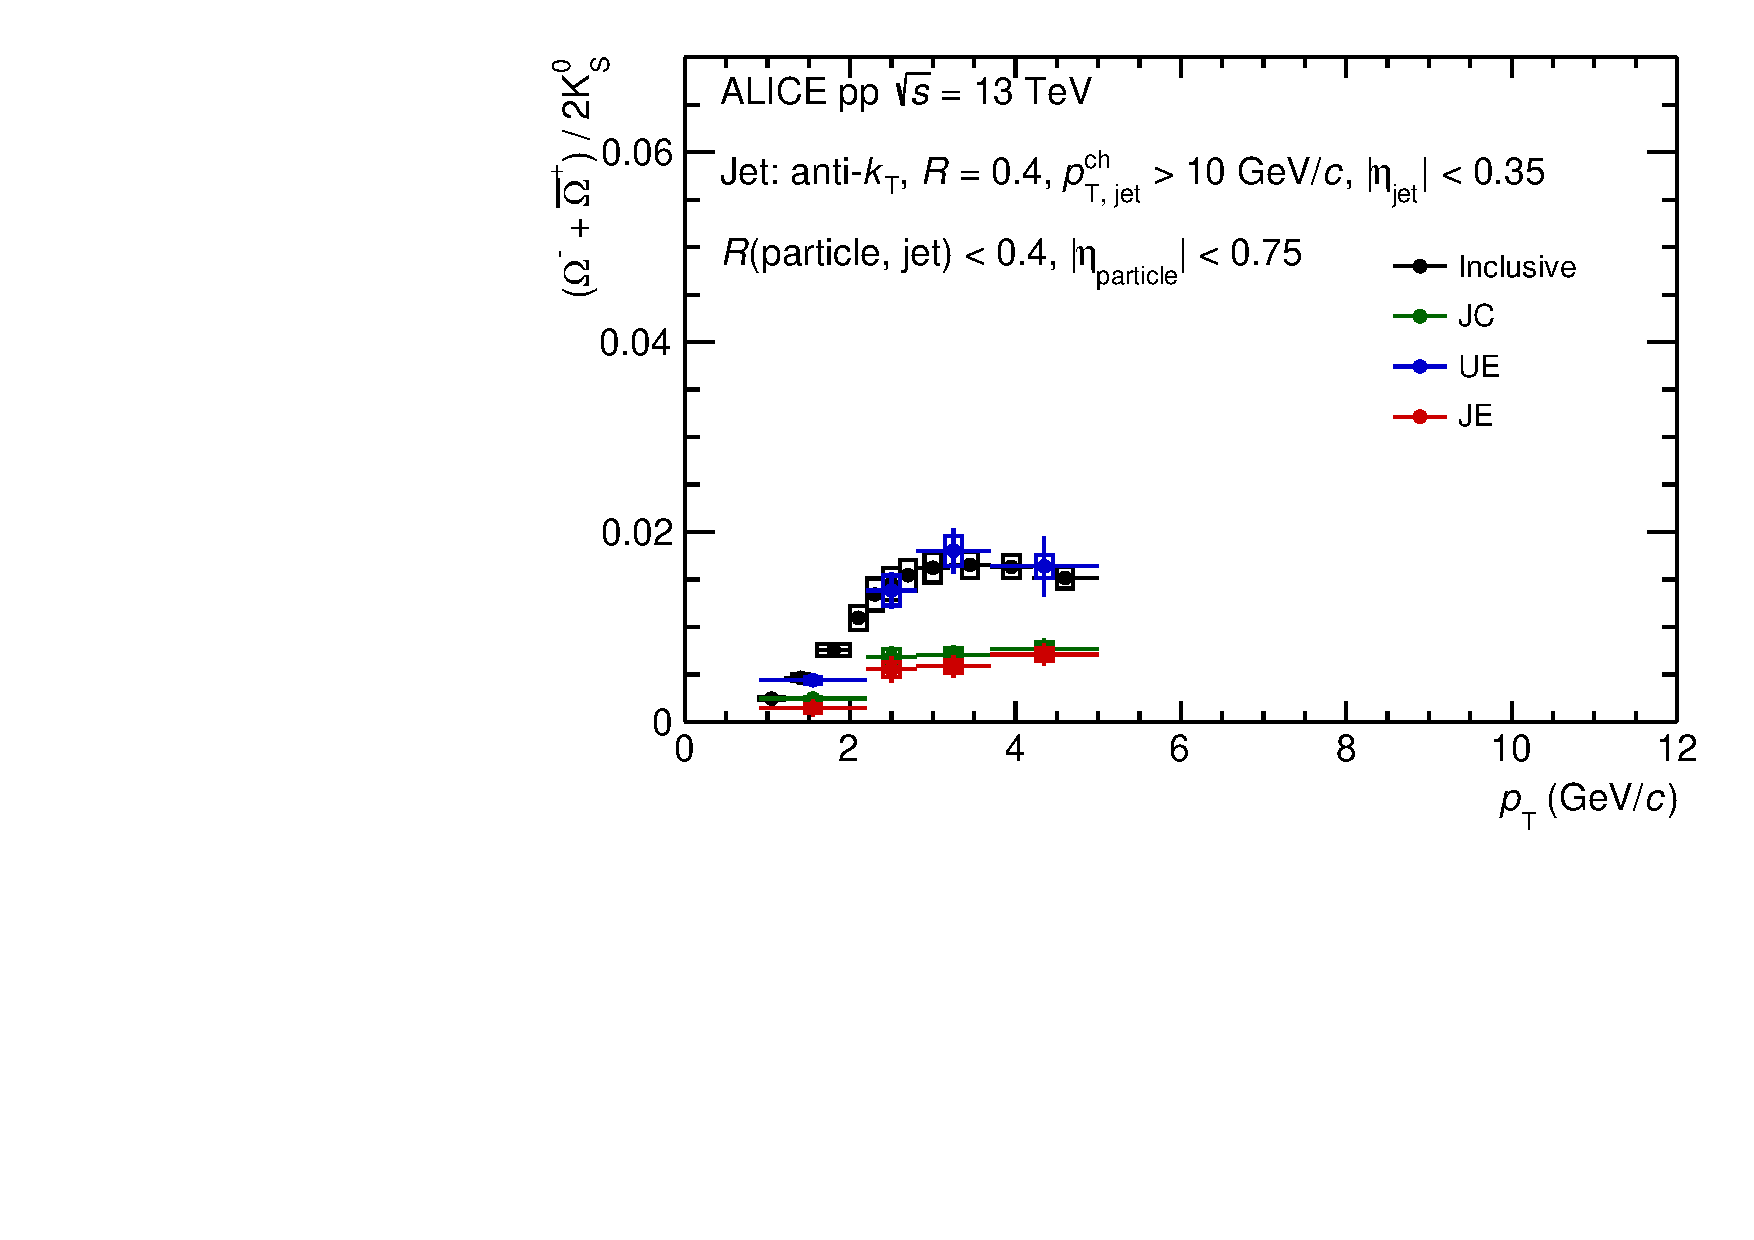
\includegraphics[width=.49\textwidth]{cf07_3}
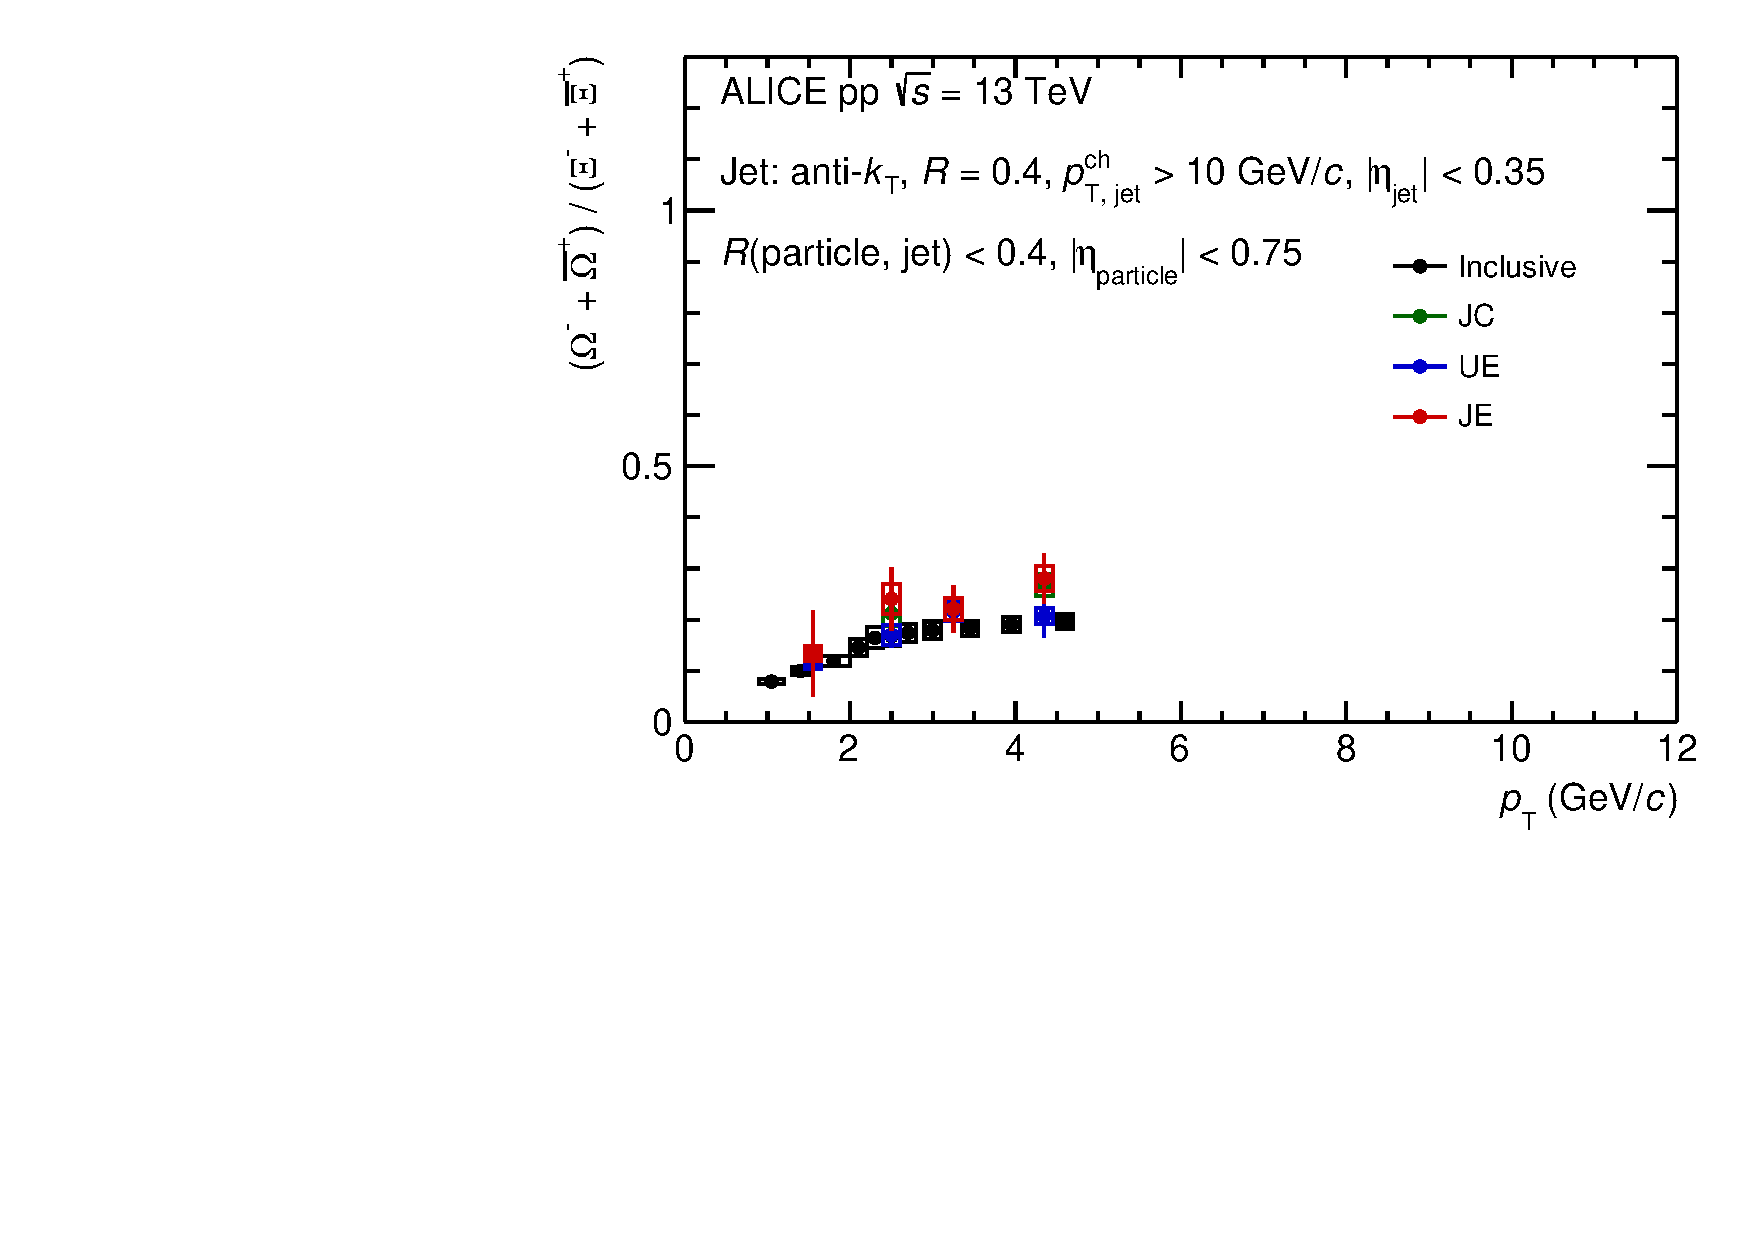
\includegraphics[width=.49\textwidth]{cf07_6}
\end{center}
\caption{The baryon-to-meson (left) and baryon-to-baryon (right) ratio as a function of particle $\pT$ in \pp collisions at \thirteen. The black points correspond to the ratio with particles from minimum bias events, the green points correspond to the ratio with particles from the jet cones, the blue points correspond to the ratio with particles ratio within a cone perpendicular to the jet, associated with the underlying event and the red points represent the ratio from the jet fragmentation. Charged-particle jets with $\pTjch > 10$~\GeVc were reconstructed with the \akT algorithm with $R = 0.4$.}
\label{fig:ppRatio}
\end{figure}

\begin{figure}[!ht]
\begin{center}
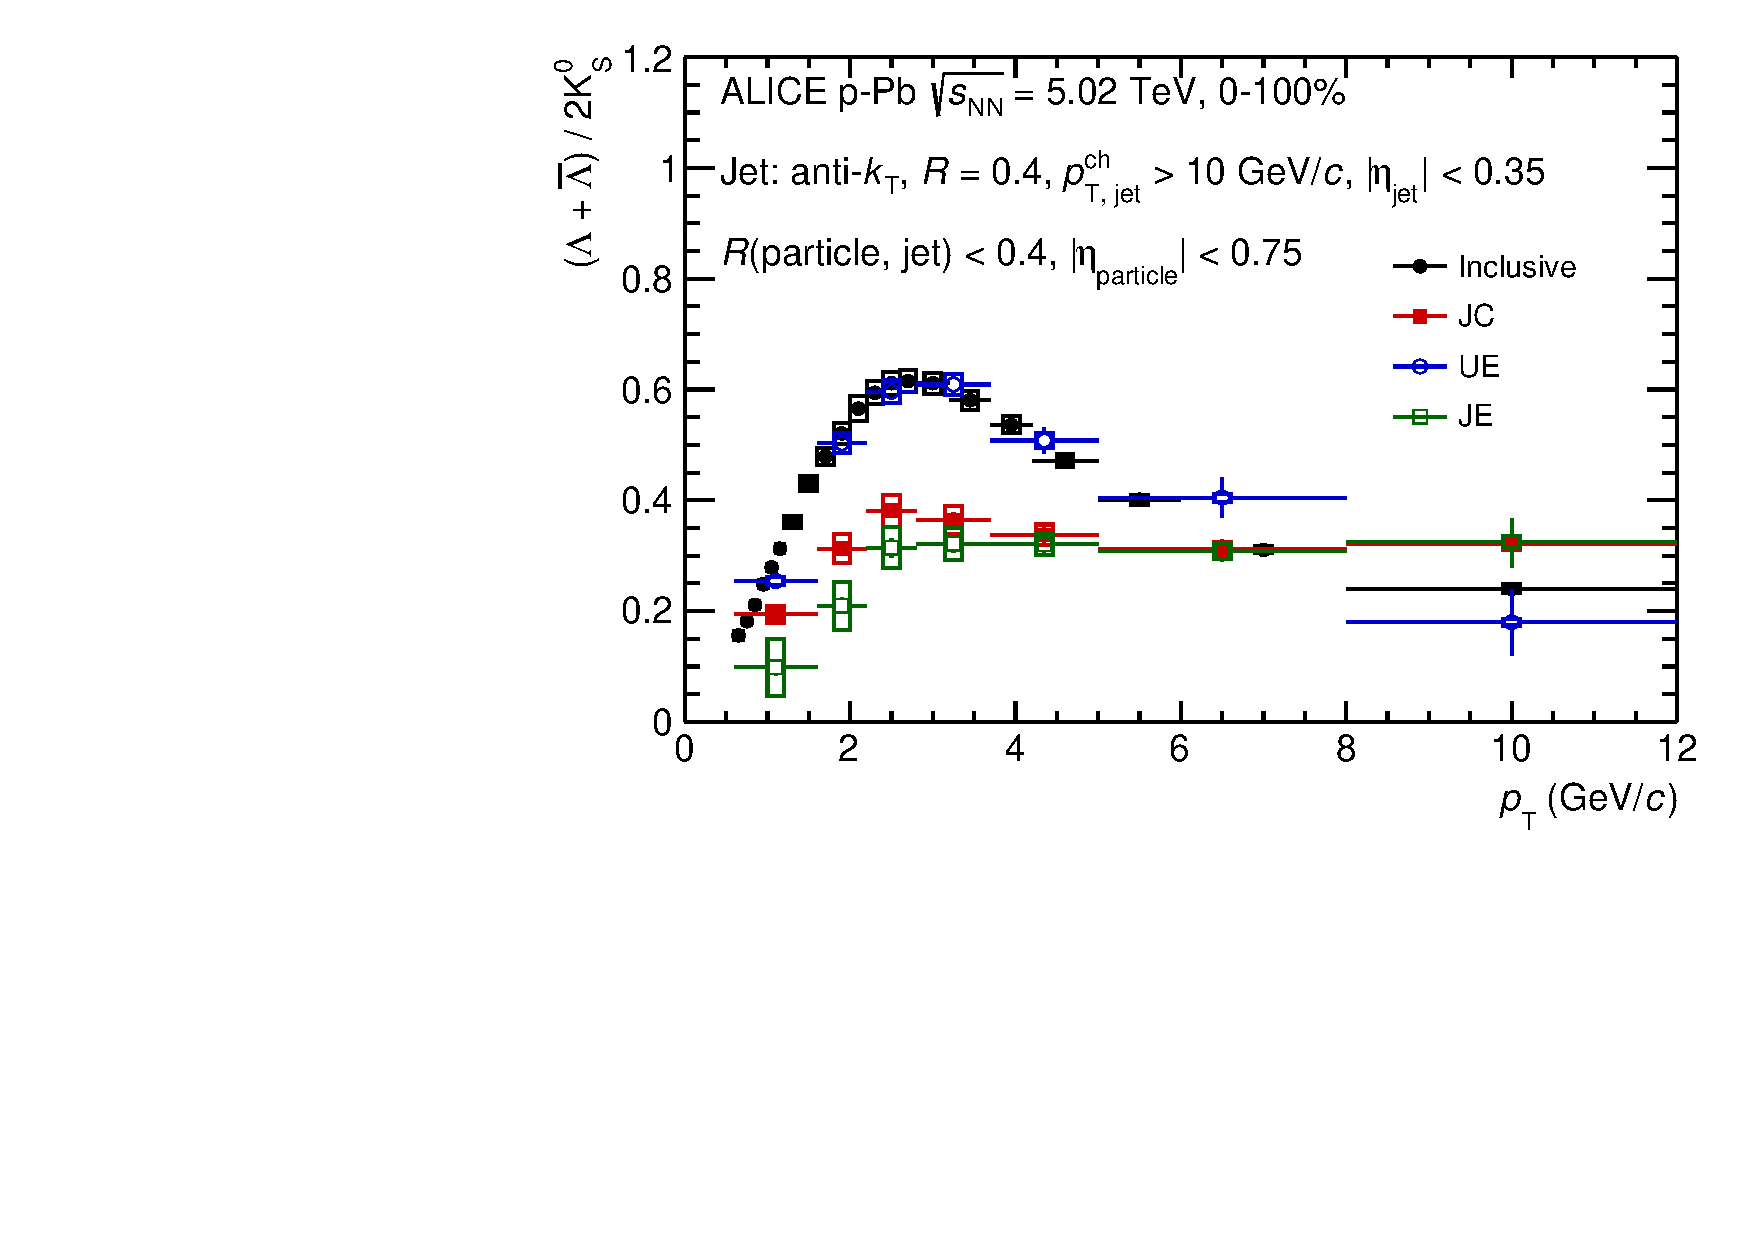
\includegraphics[width=.49\textwidth]{cf08_1}
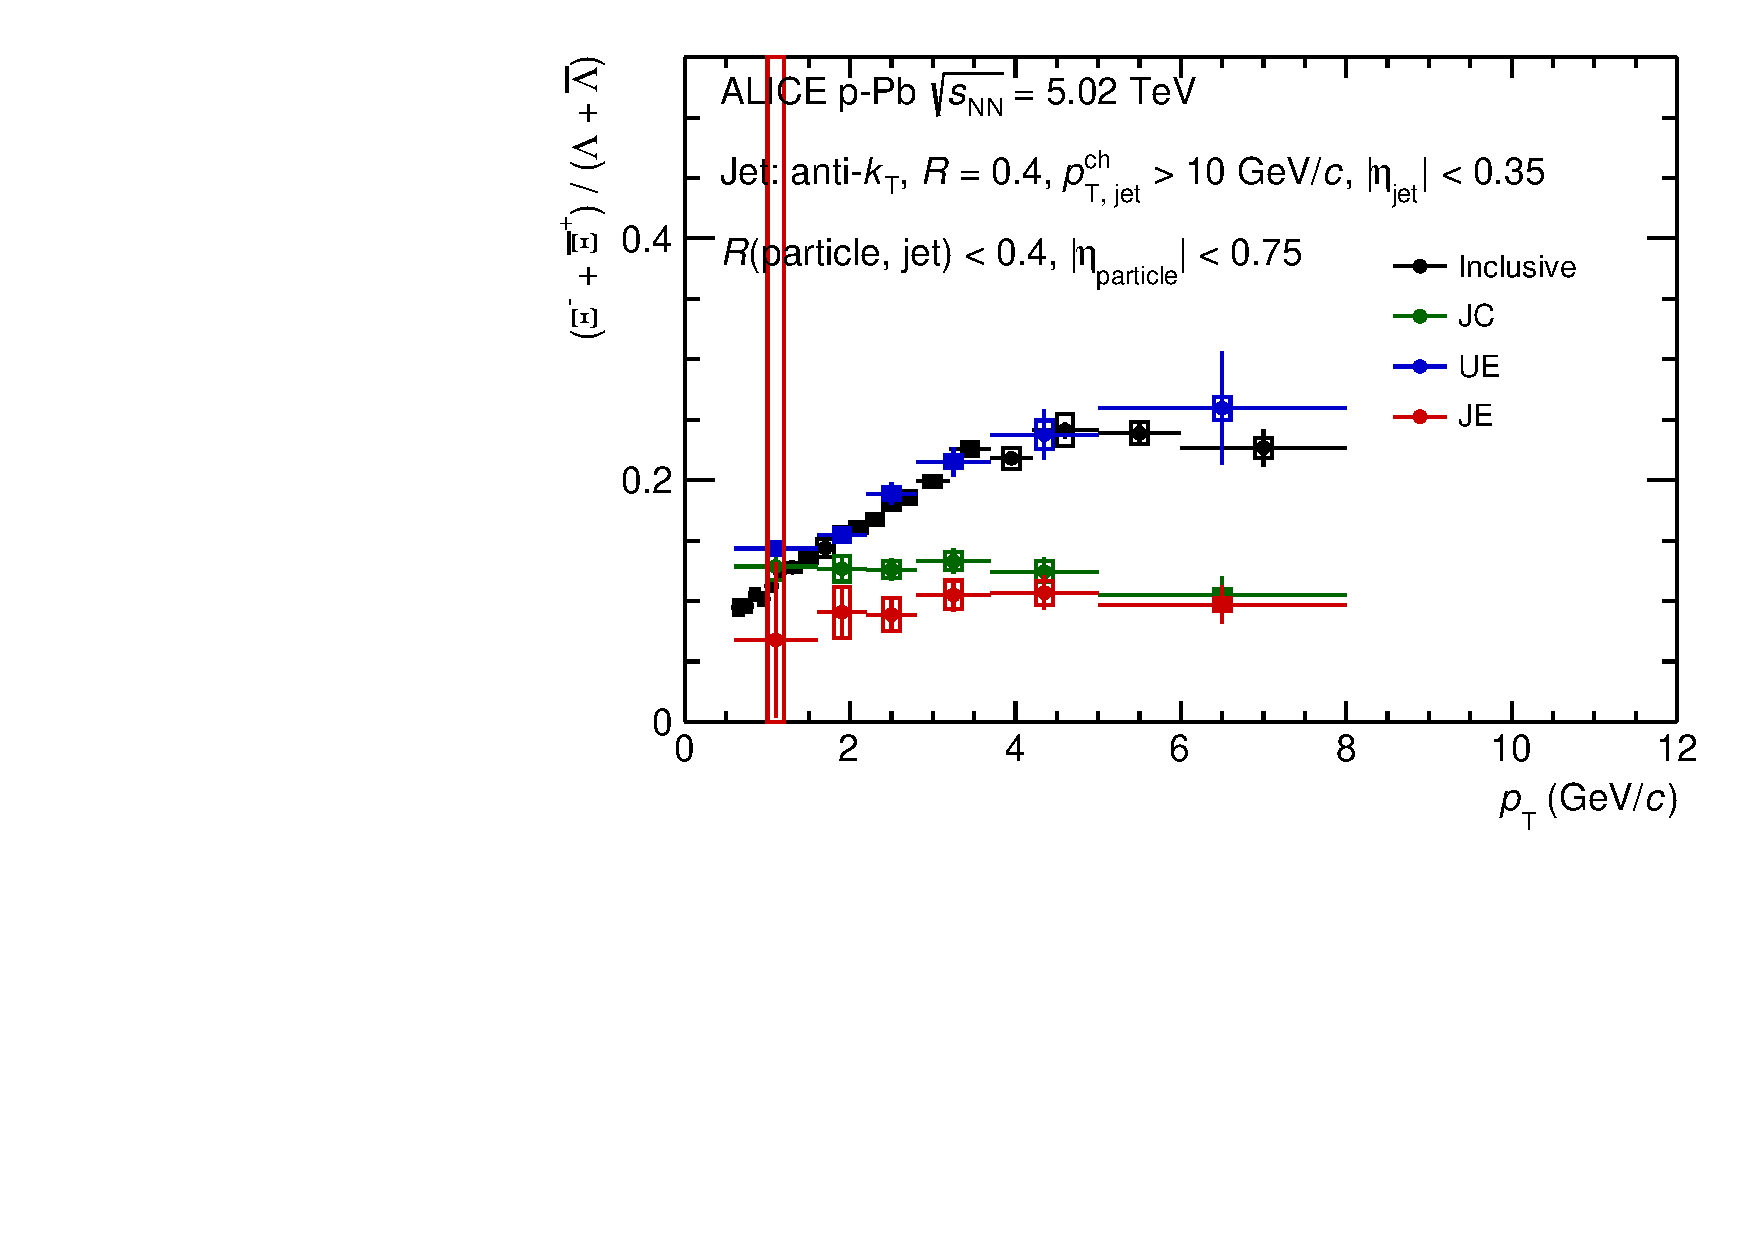
\includegraphics[width=.49\textwidth]{cf08_4}
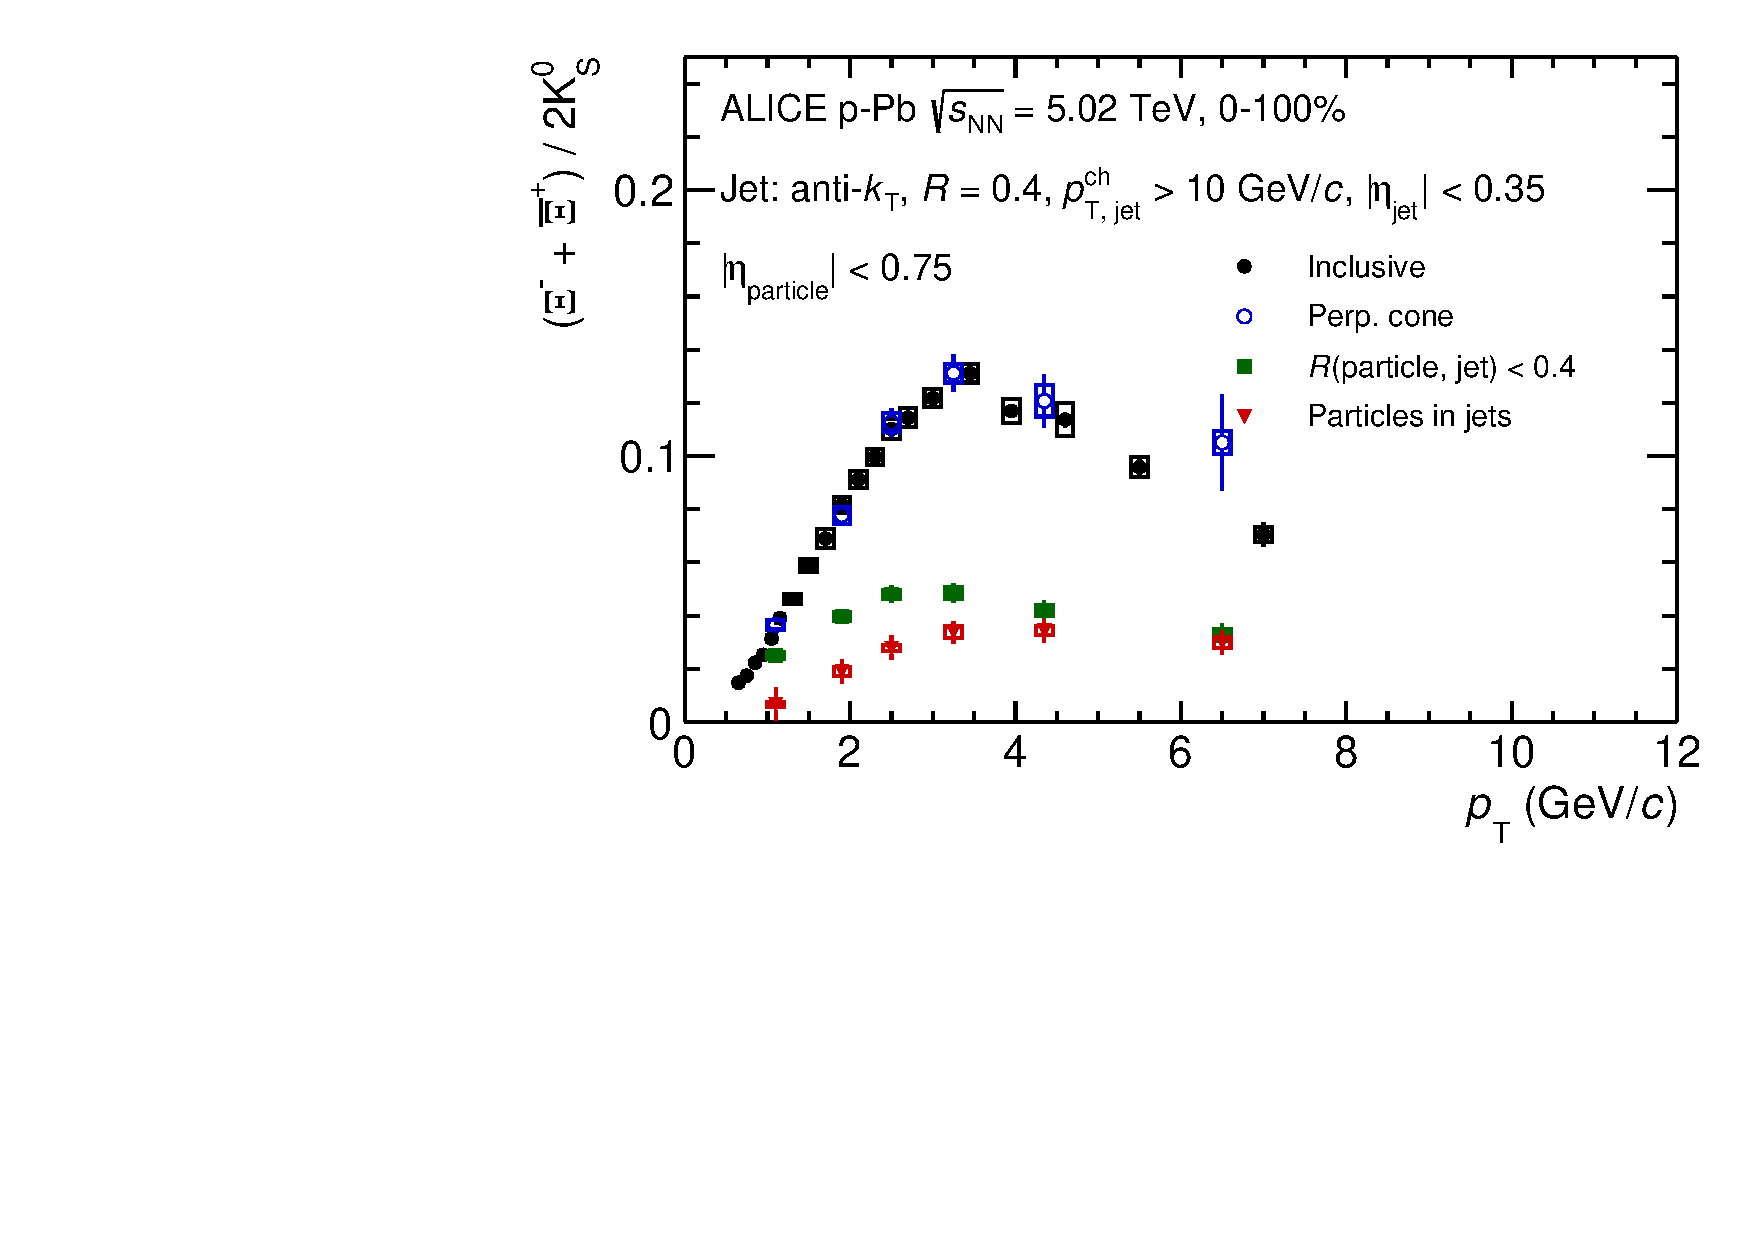
\includegraphics[width=.49\textwidth]{cf08_2}
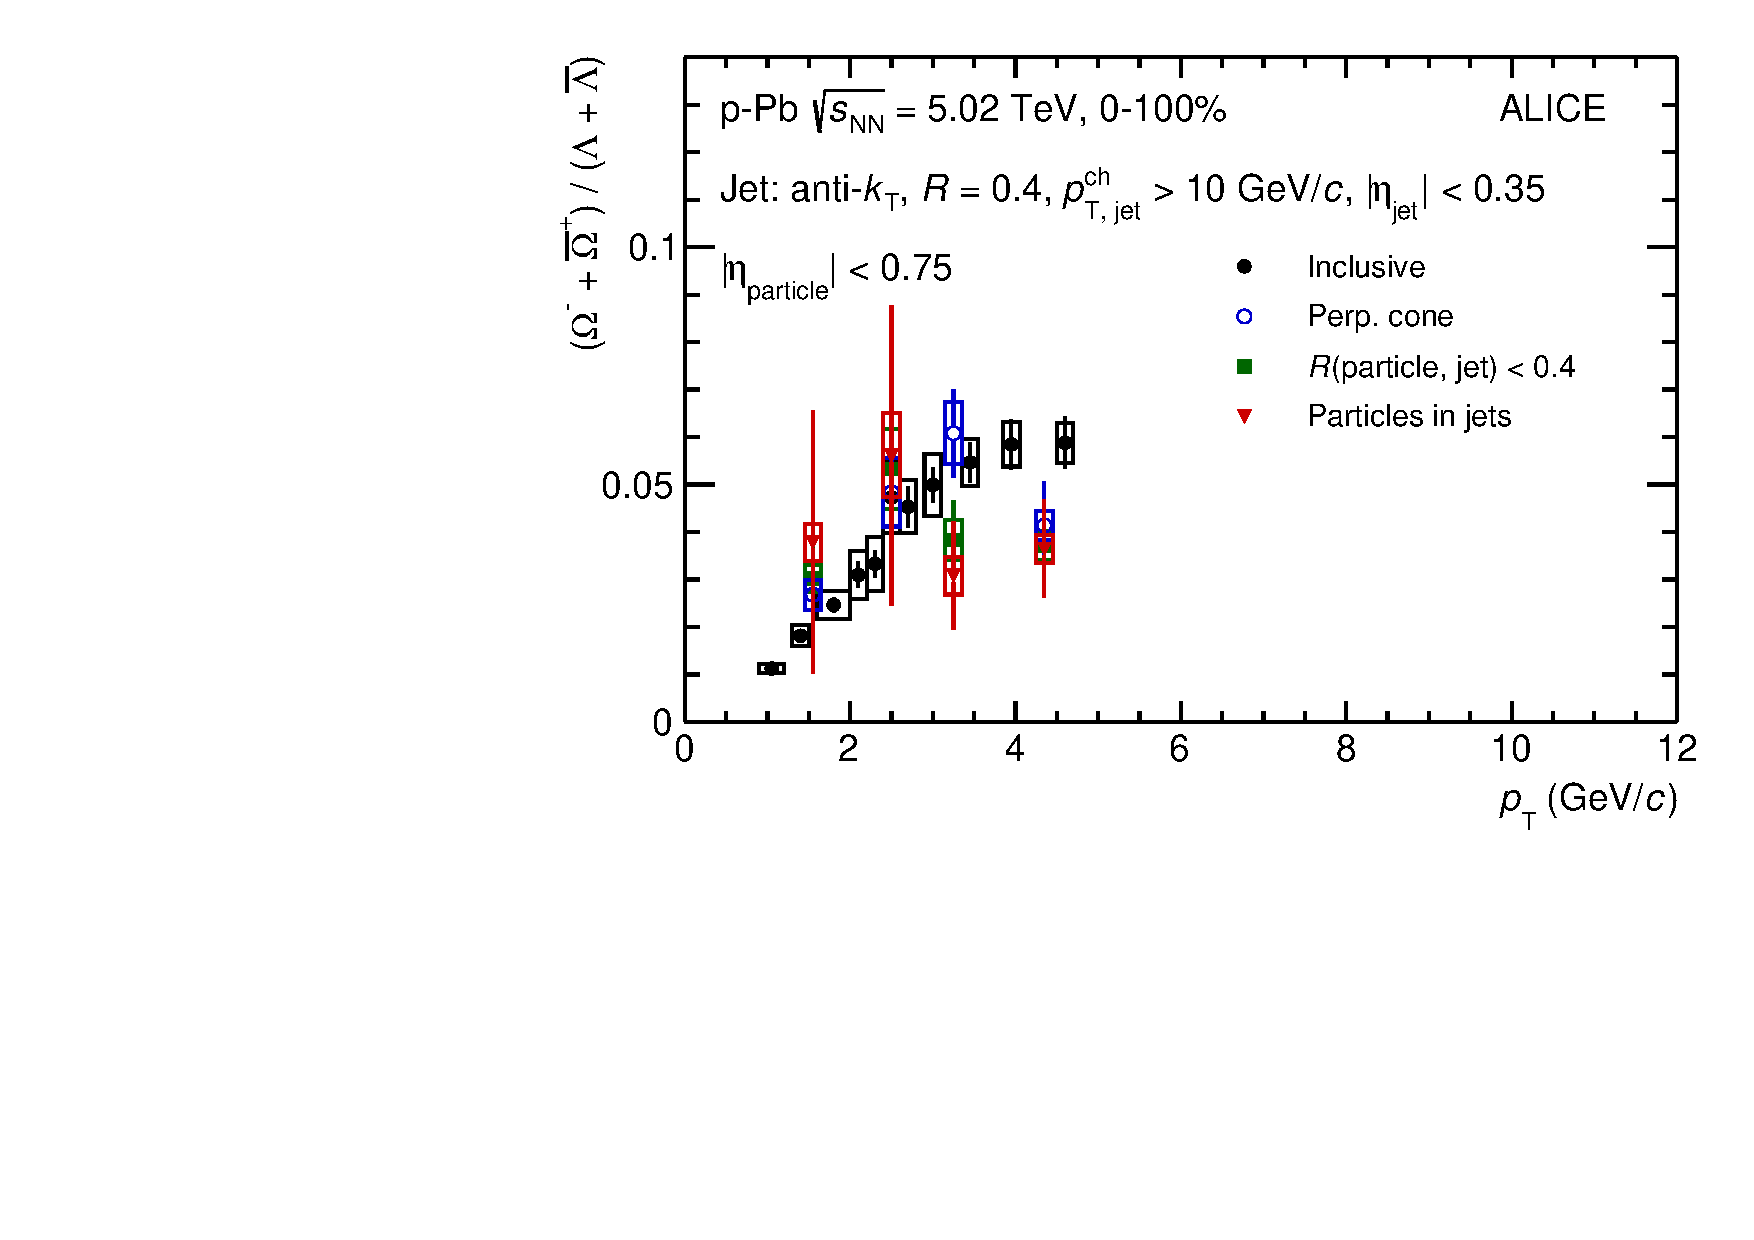
\includegraphics[width=.49\textwidth]{cf08_5}
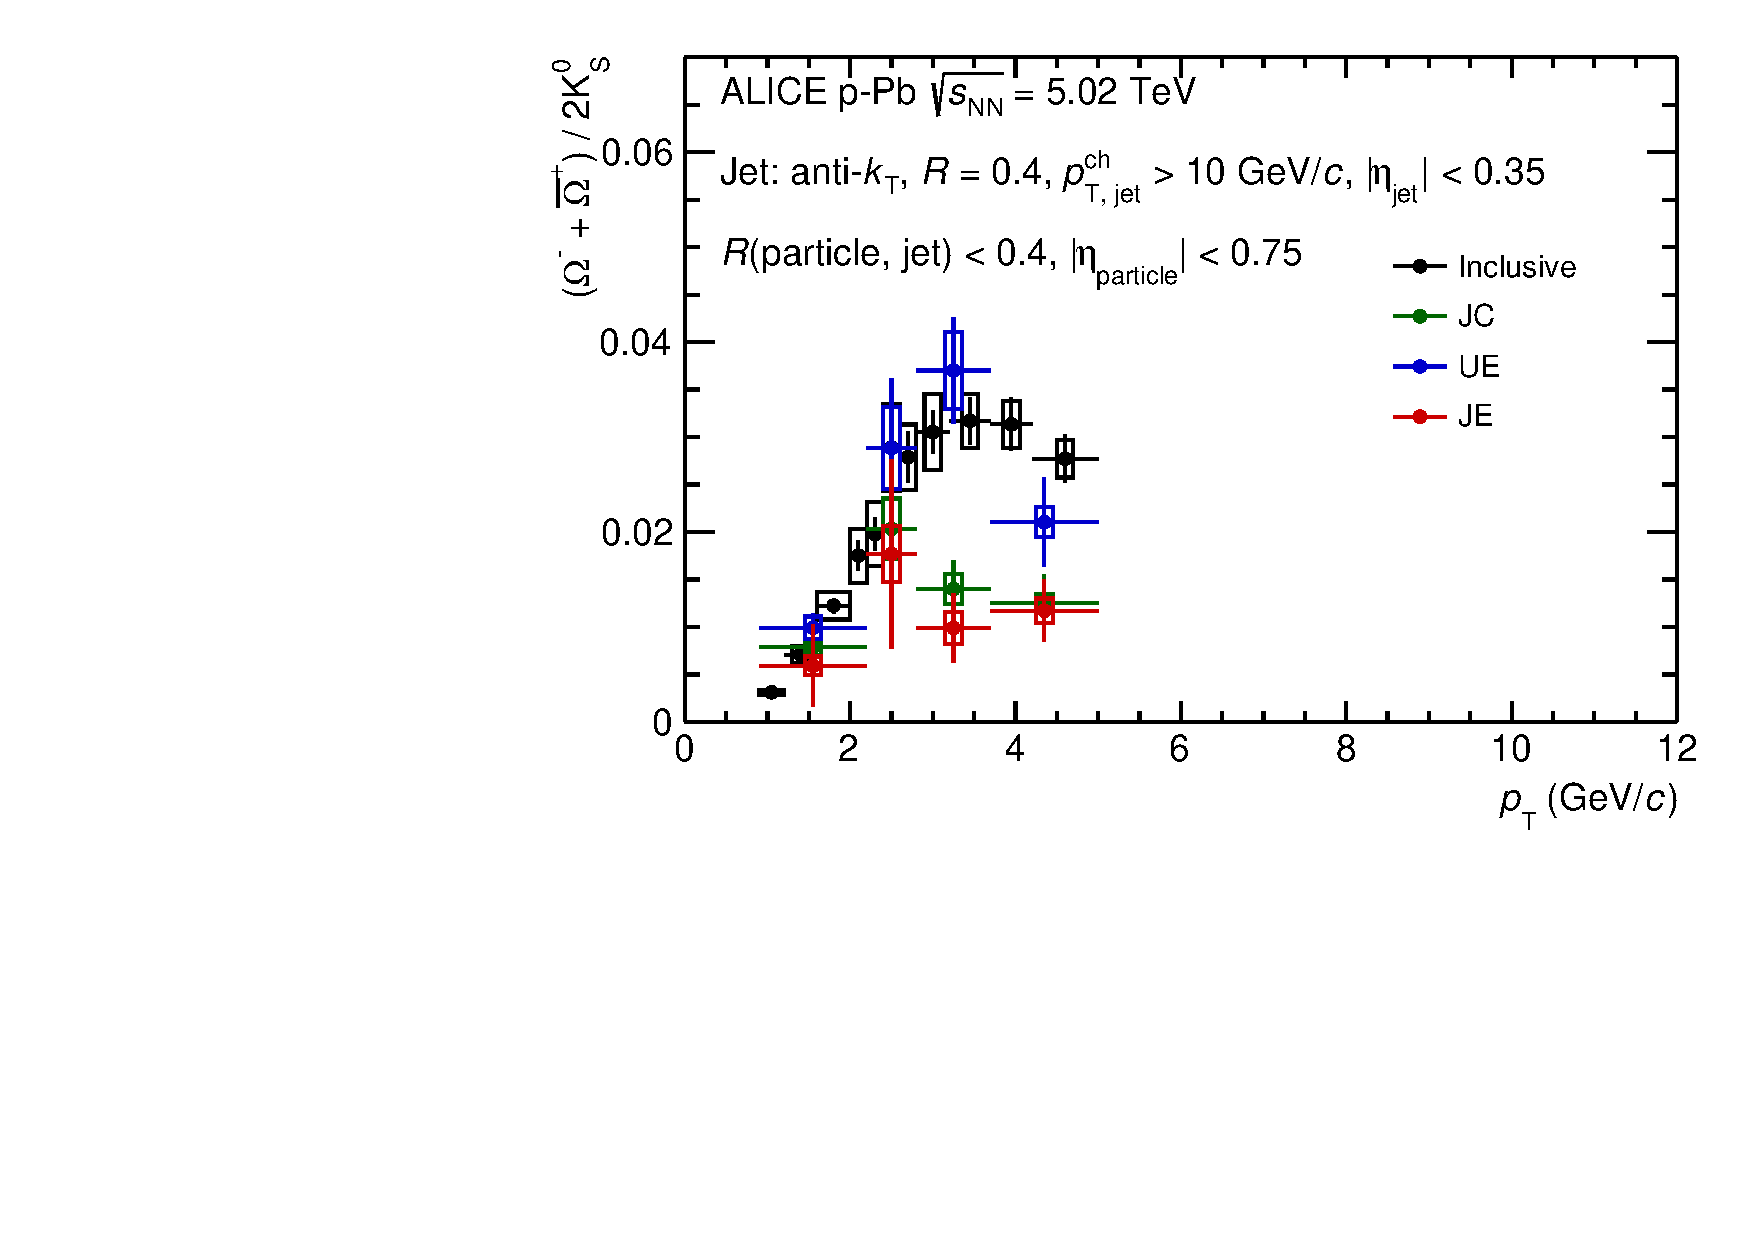
\includegraphics[width=.49\textwidth]{cf08_3}
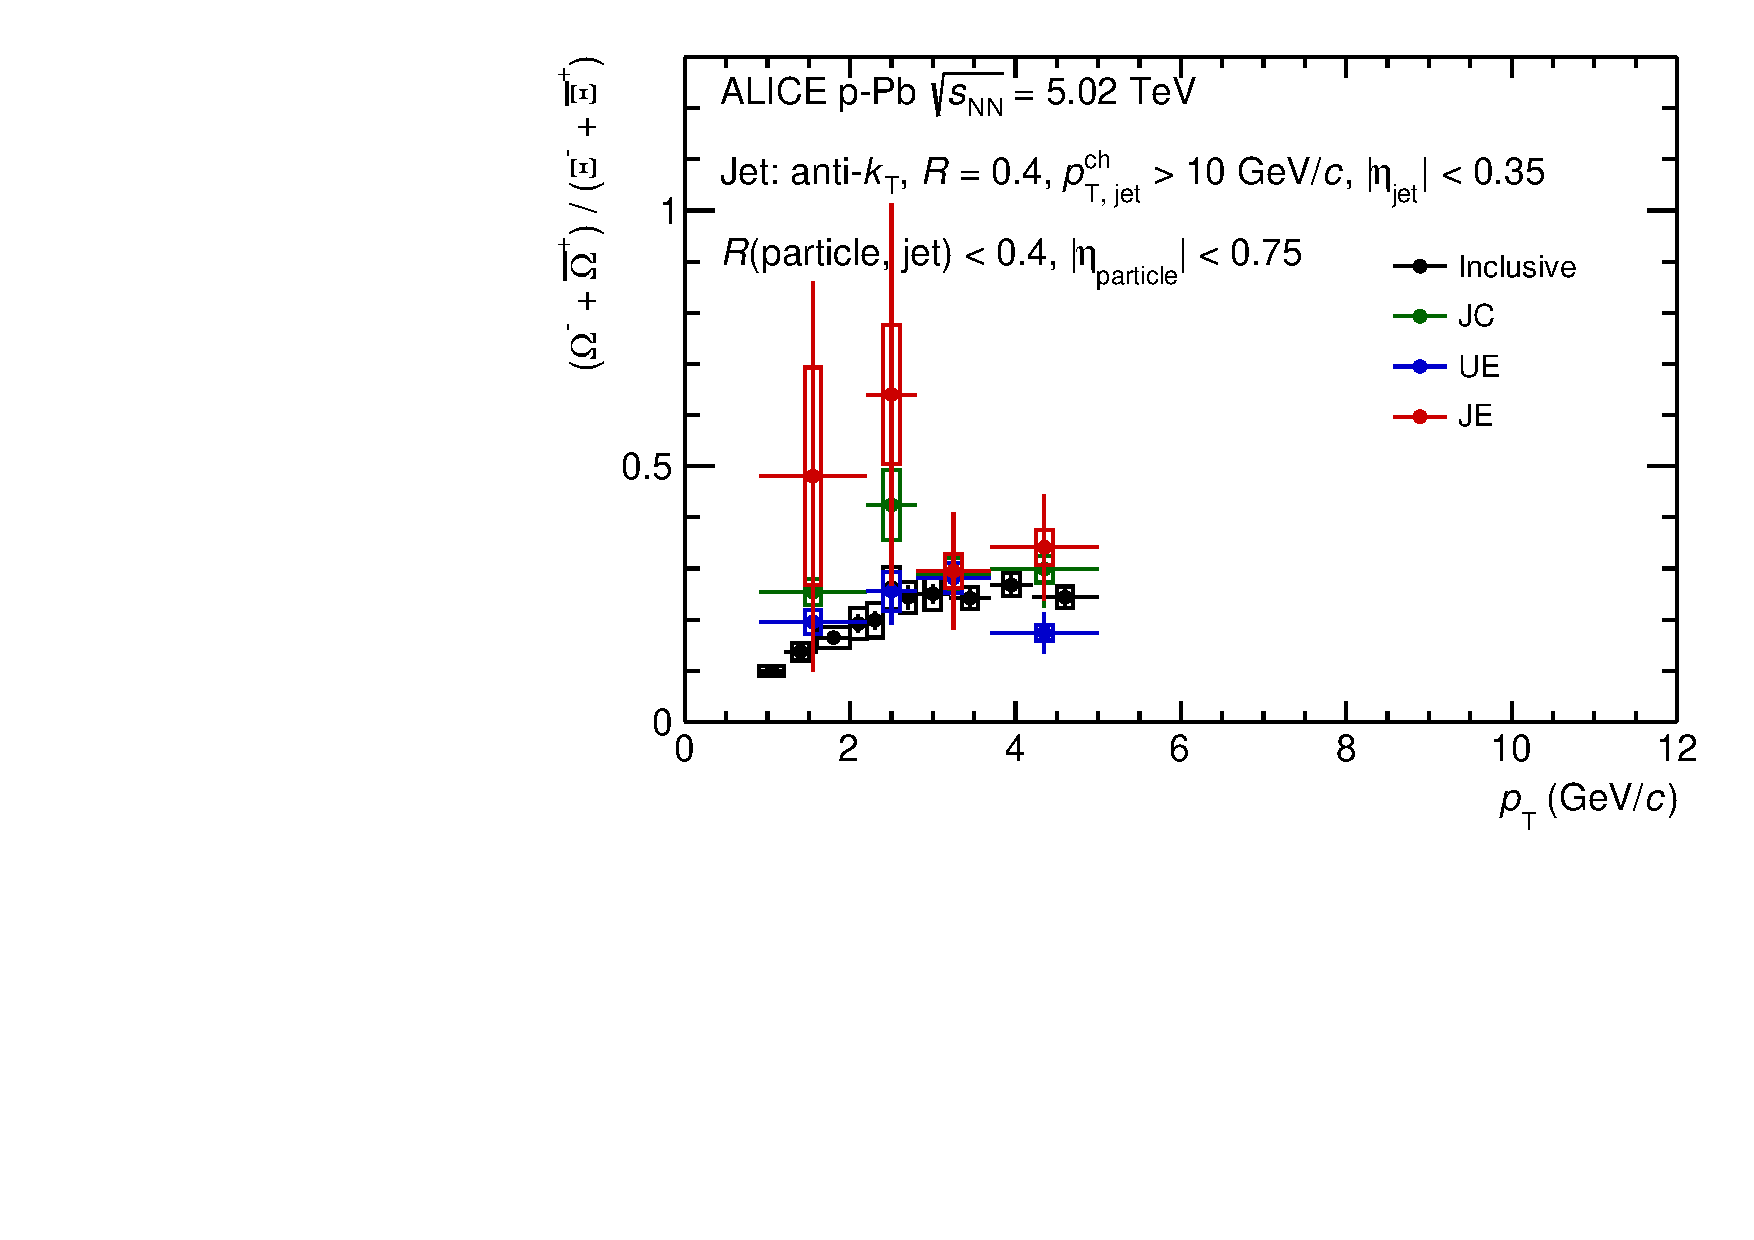
\includegraphics[width=.49\textwidth]{cf08_6}
\end{center}
\caption{The baryon-to-meson (left) and baryon-to-baryon (right) ratio as a function of particle $\pT$ in \pPb collisions at \fivenn. The black points correspond to the ratio with particles from minimum bias events, the green points correspond to the ratio with particles from the jet cones, the blue points correspond to the ratio with particles ratio within a cone perpendicular to the jet, associated with the underlying event and the red points represent the ratio from the jet fragmentation. Charged-particle jets with $\pTjch > 10$~\GeVc were reconstructed with the \akT algorithm with $R = 0.4$.}
\label{fig:pPbRatio}
\end{figure}

Fig.~\ref{fig:pppPbRatio} shows the particle ratios in jet in \pp collisions and in the different multiplicity classes in \pPb collisions for the same selection of the matching radius $R(\rm{particle, jet}) < 0.4$ in both systems.
The systematic uncertainties~(open boxes) are uncorrelated between the systems.
The particle ratios in the jet are observed to be relatively multiplicity class and system independent.
It is noteworthy that the baryon-to-meson ($\lmb/\kzero$, $\Xi/\kzero$ and $\Omega/\kzero$) ratios have a hint of multiplicity (collision system) dependence for $2 < \pT < 4$~\GeVc, however the difference between the ratios is less than $2\sigma$ and the measurement is currently dominated by large uncertainties.
For $\pT > 5$~\GeVc, the baryon-to-meson ratios become consistent for all multiplicity classes and collision systems.
In the Fig~\ref{fig:pppPbRatio}, these ratios are compared to the PYTHIA 8 simulation with Monash tune. Due to the PYTHIA overestimate with ($\X + \Ix$) (see Fig.~\ref{fig:pPbSpectwCent}) in jet spectra. So here we observed the PYTHIA can simulate the $(\lmb + \almb)/2\kzero$ well but not for the ratios which correlated with multi-strange particles.

\begin{figure}[!ht]
\begin{center}
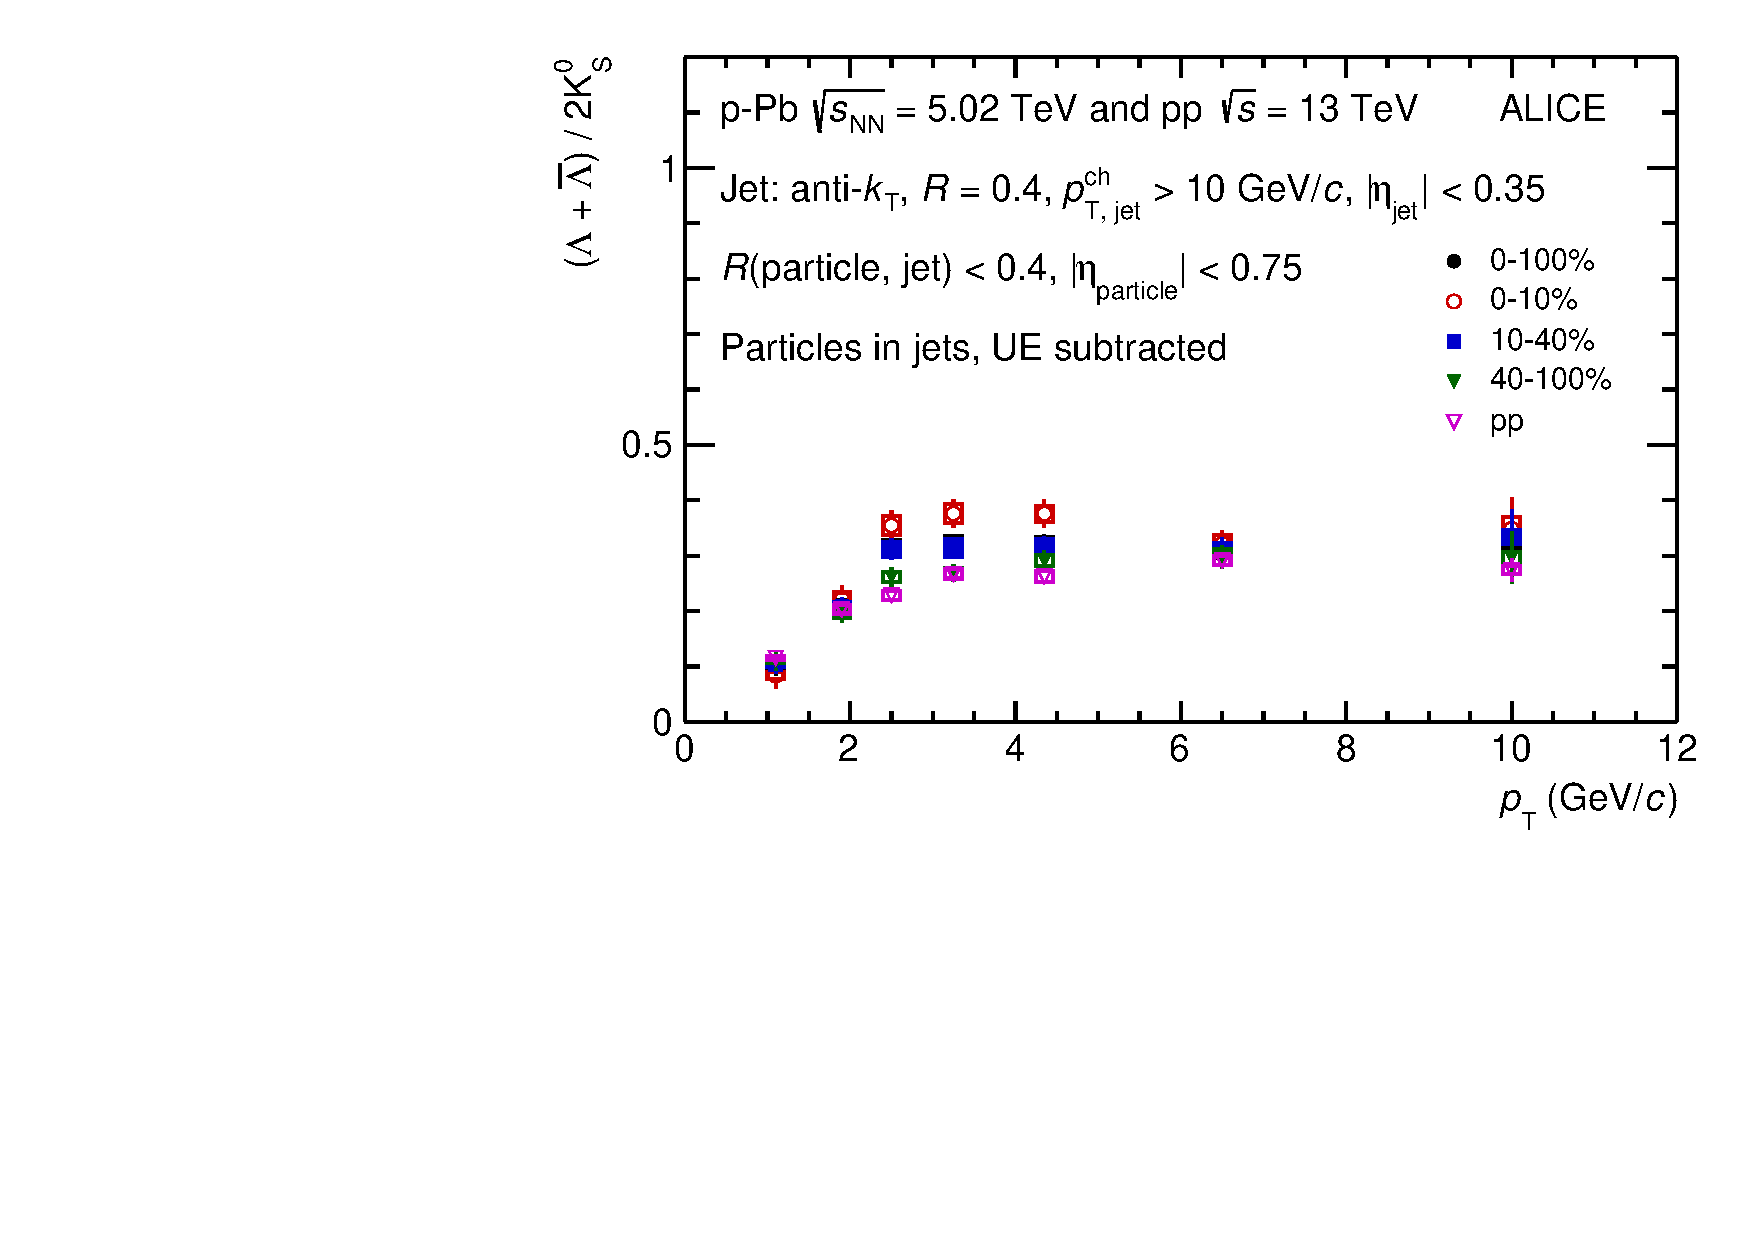
\includegraphics[width=.49\textwidth]{cf09_1}
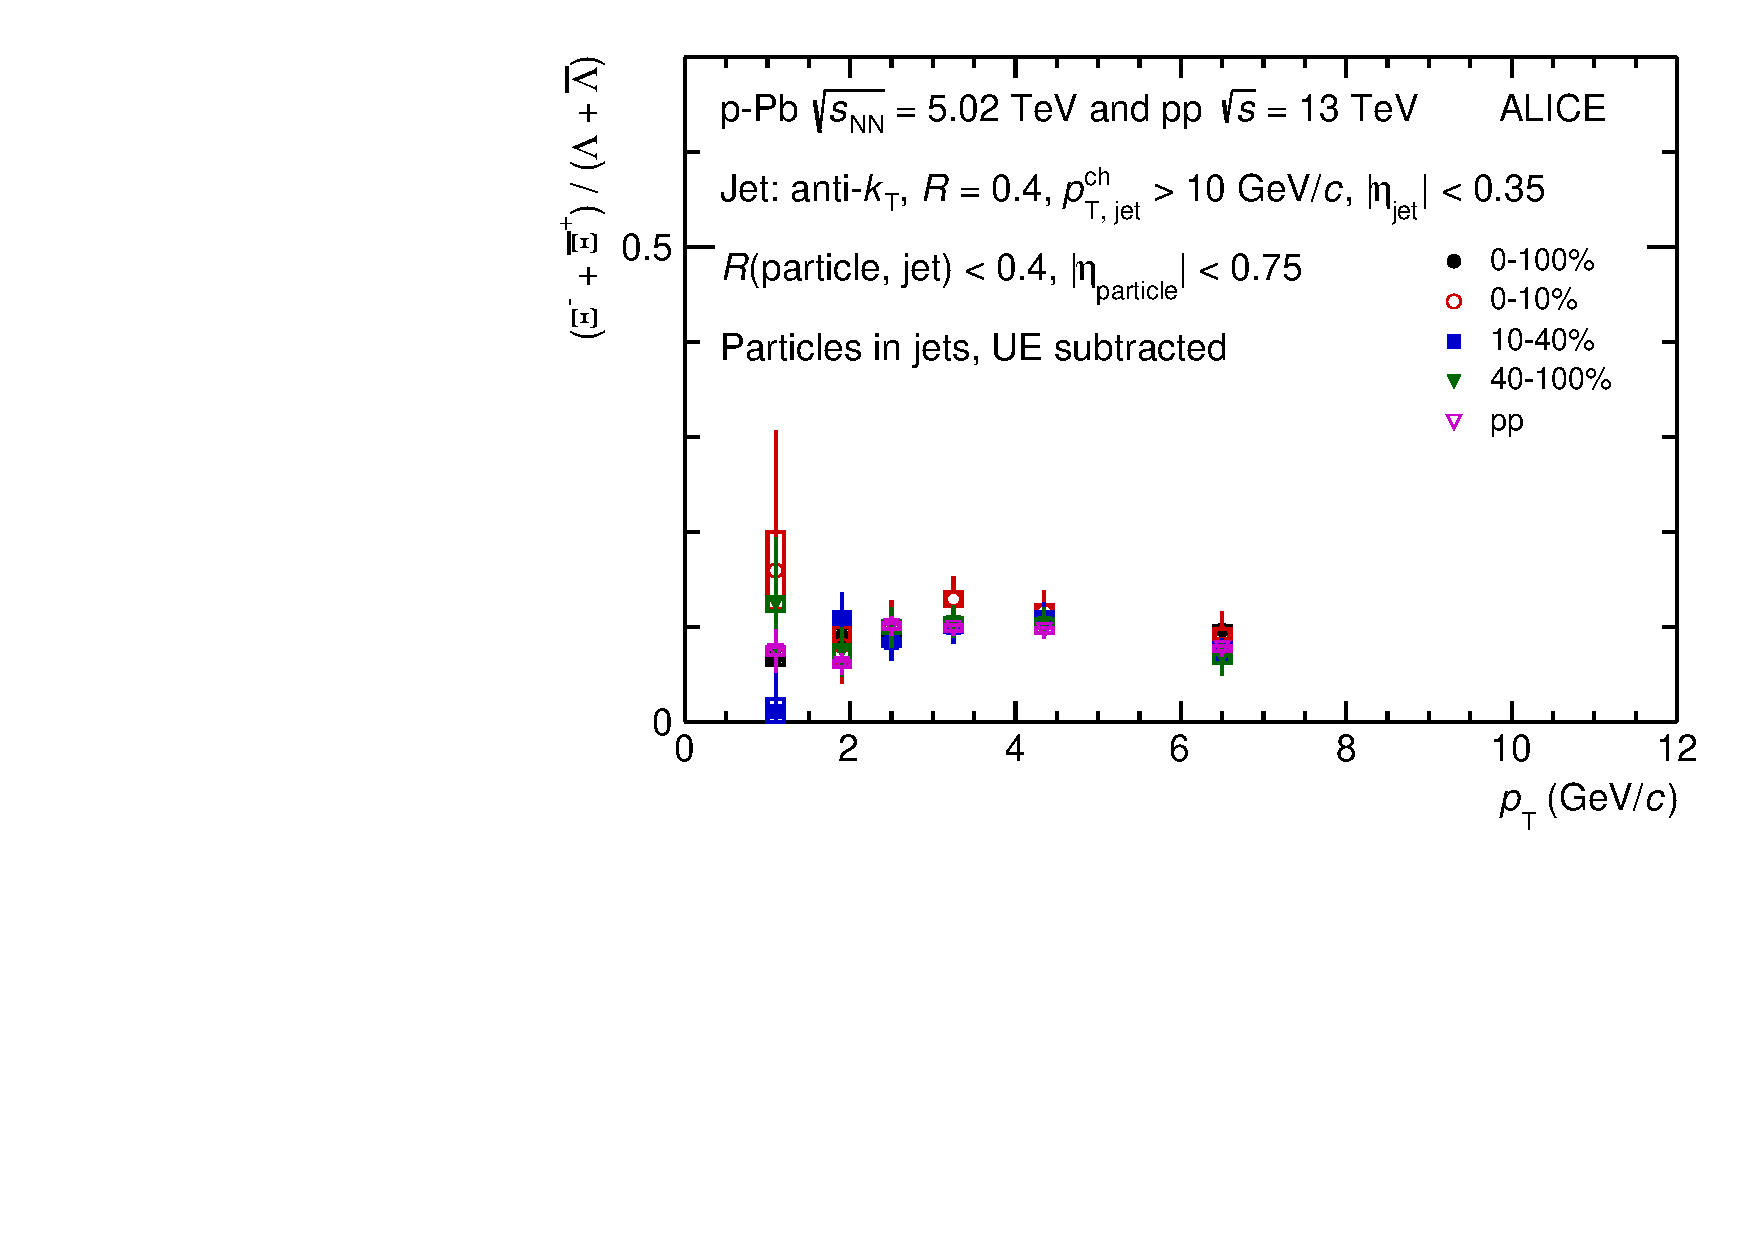
\includegraphics[width=.49\textwidth]{cf09_4}
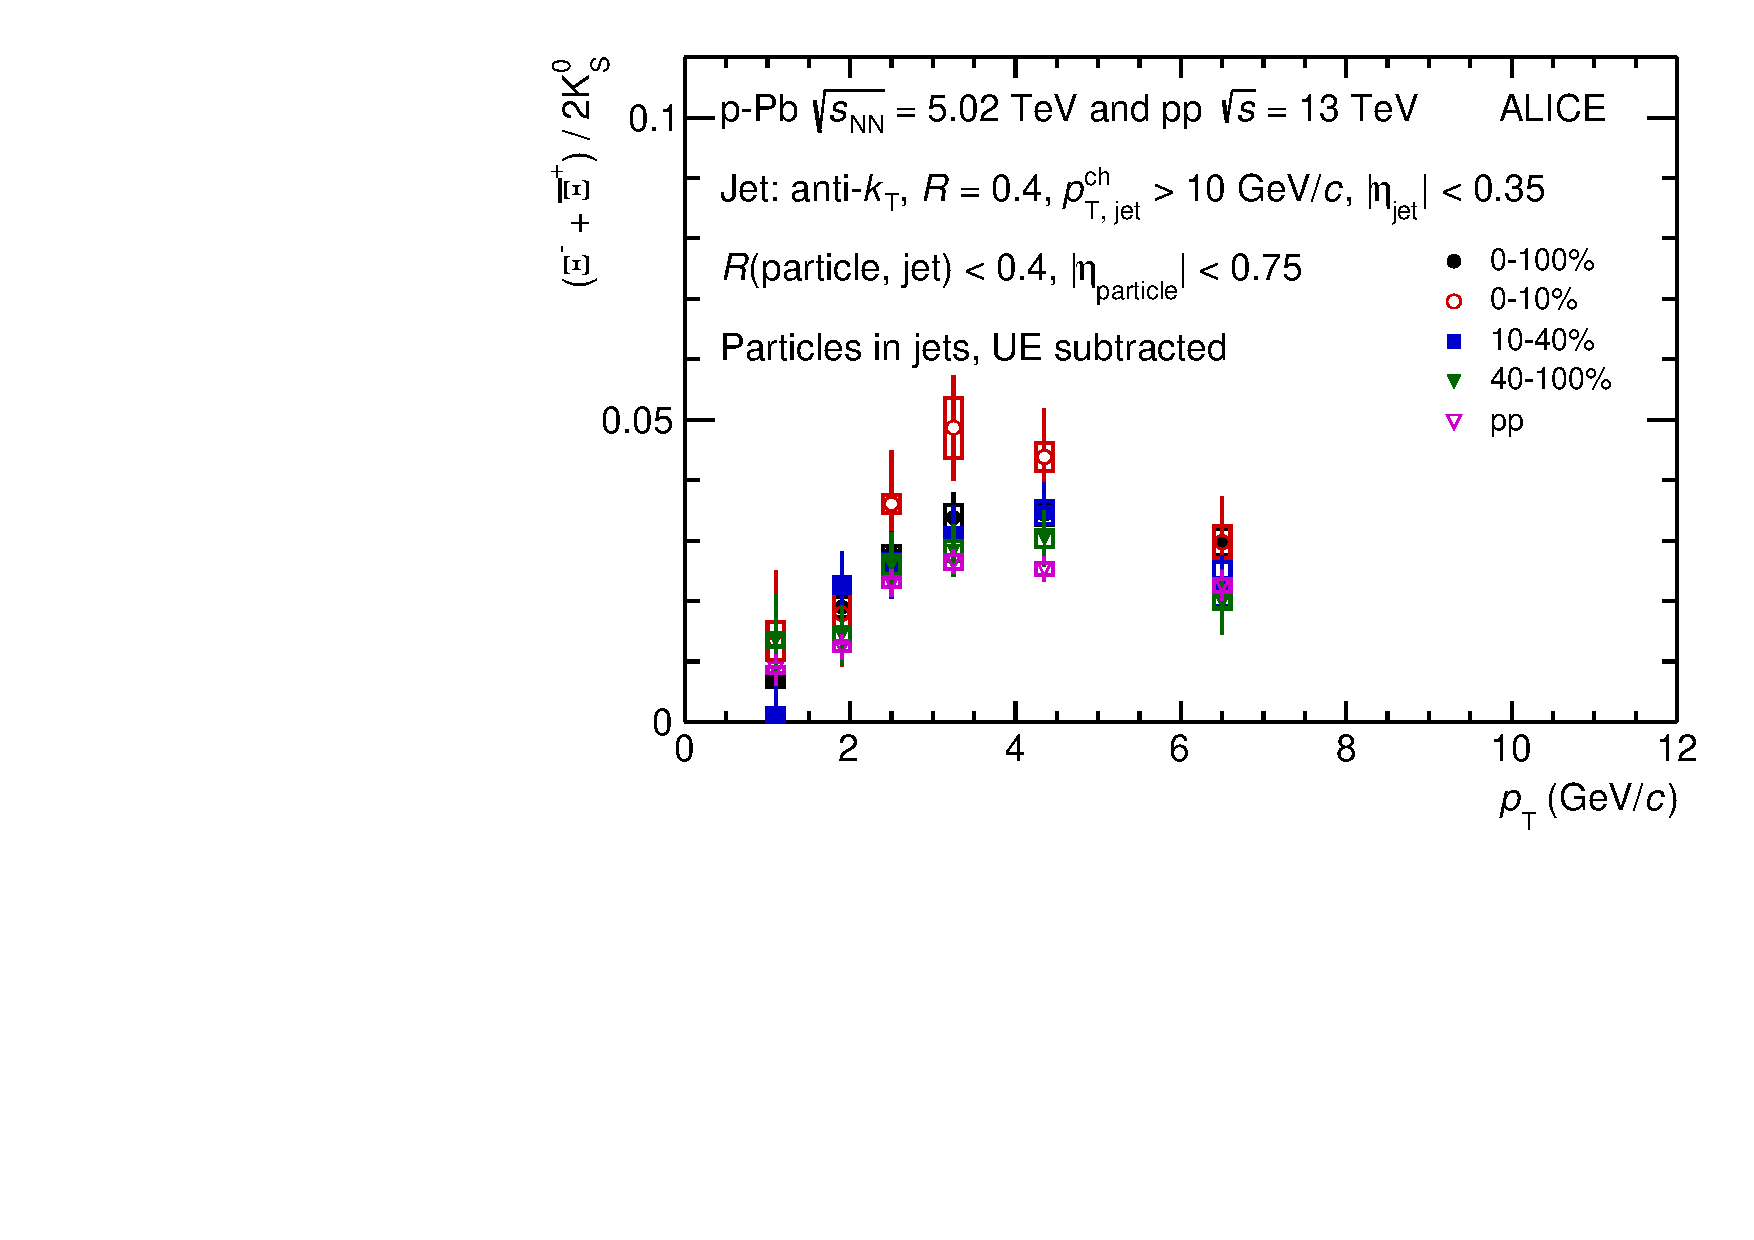
\includegraphics[width=.49\textwidth]{cf09_2}
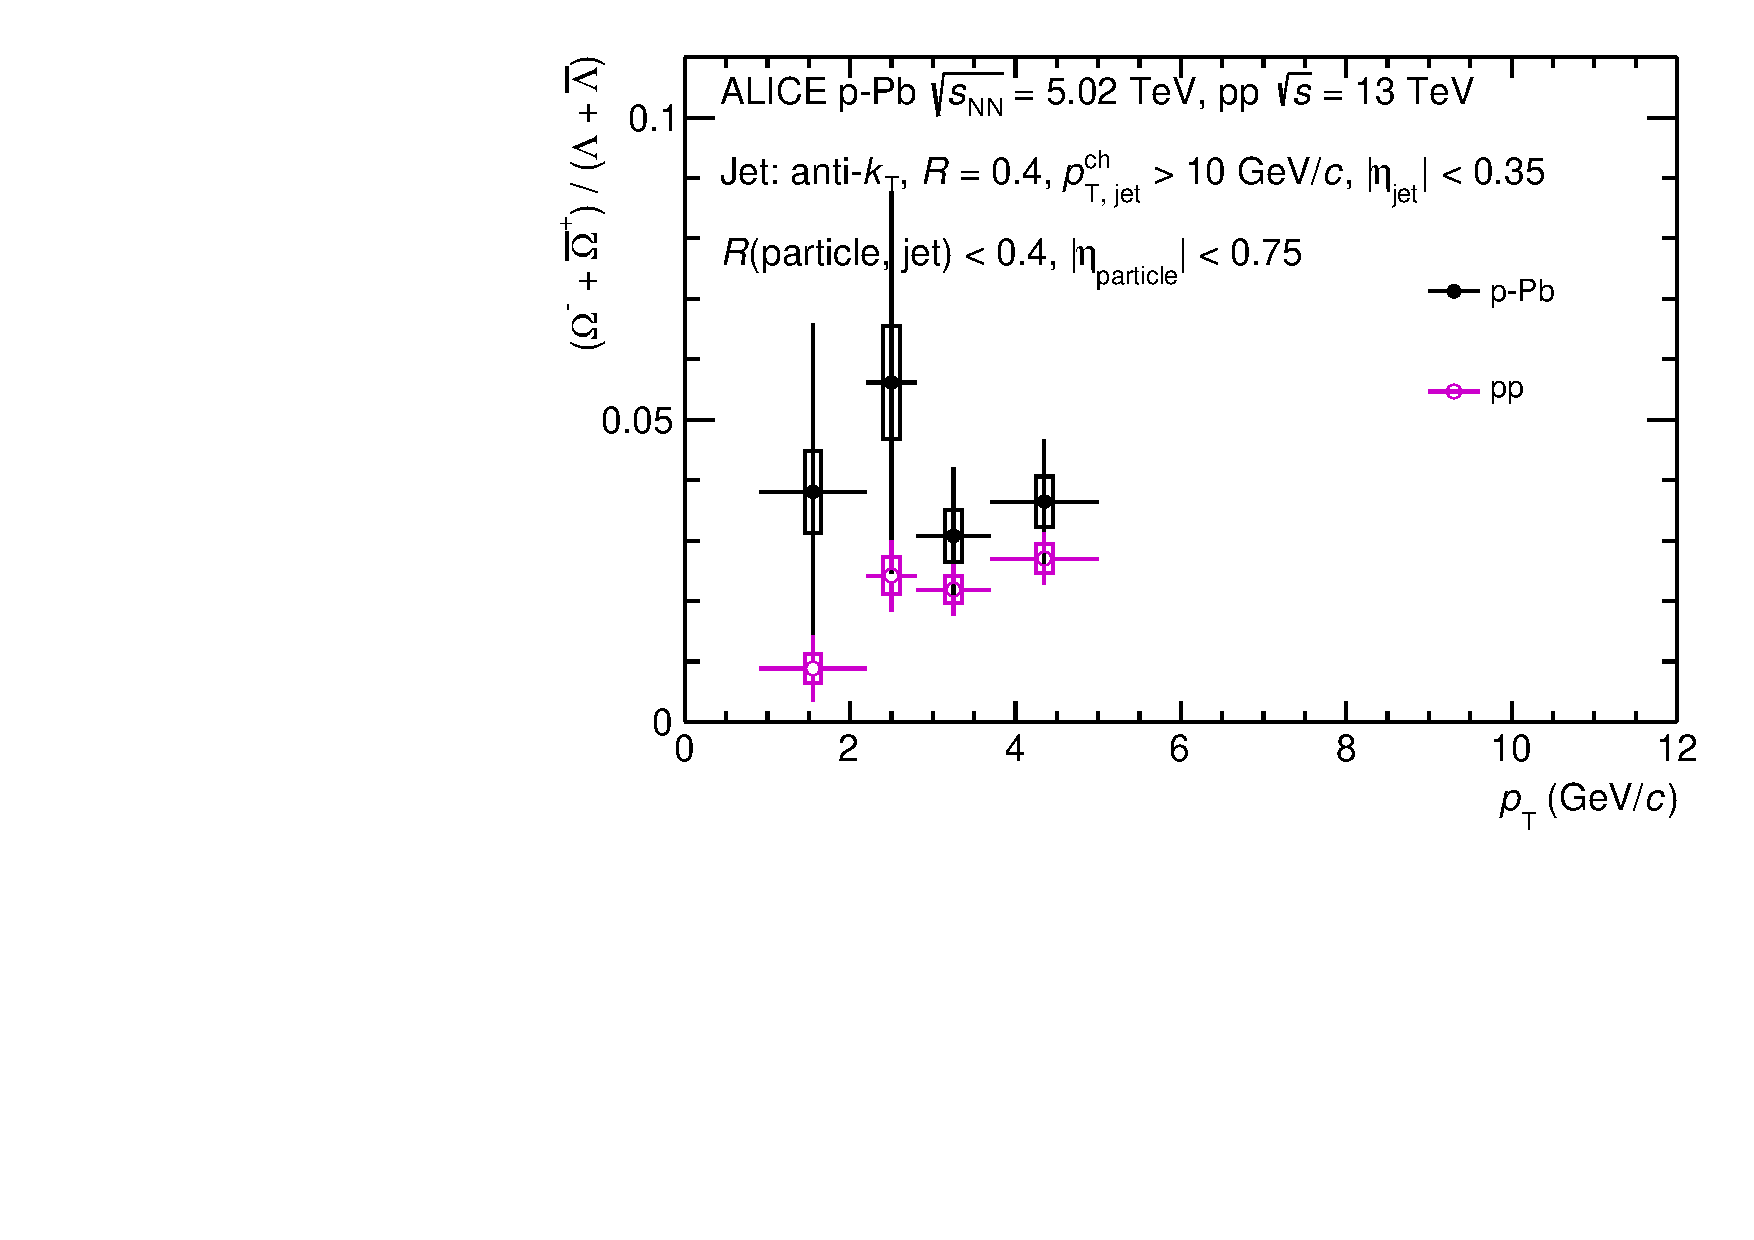
\includegraphics[width=.49\textwidth]{cf09_5}
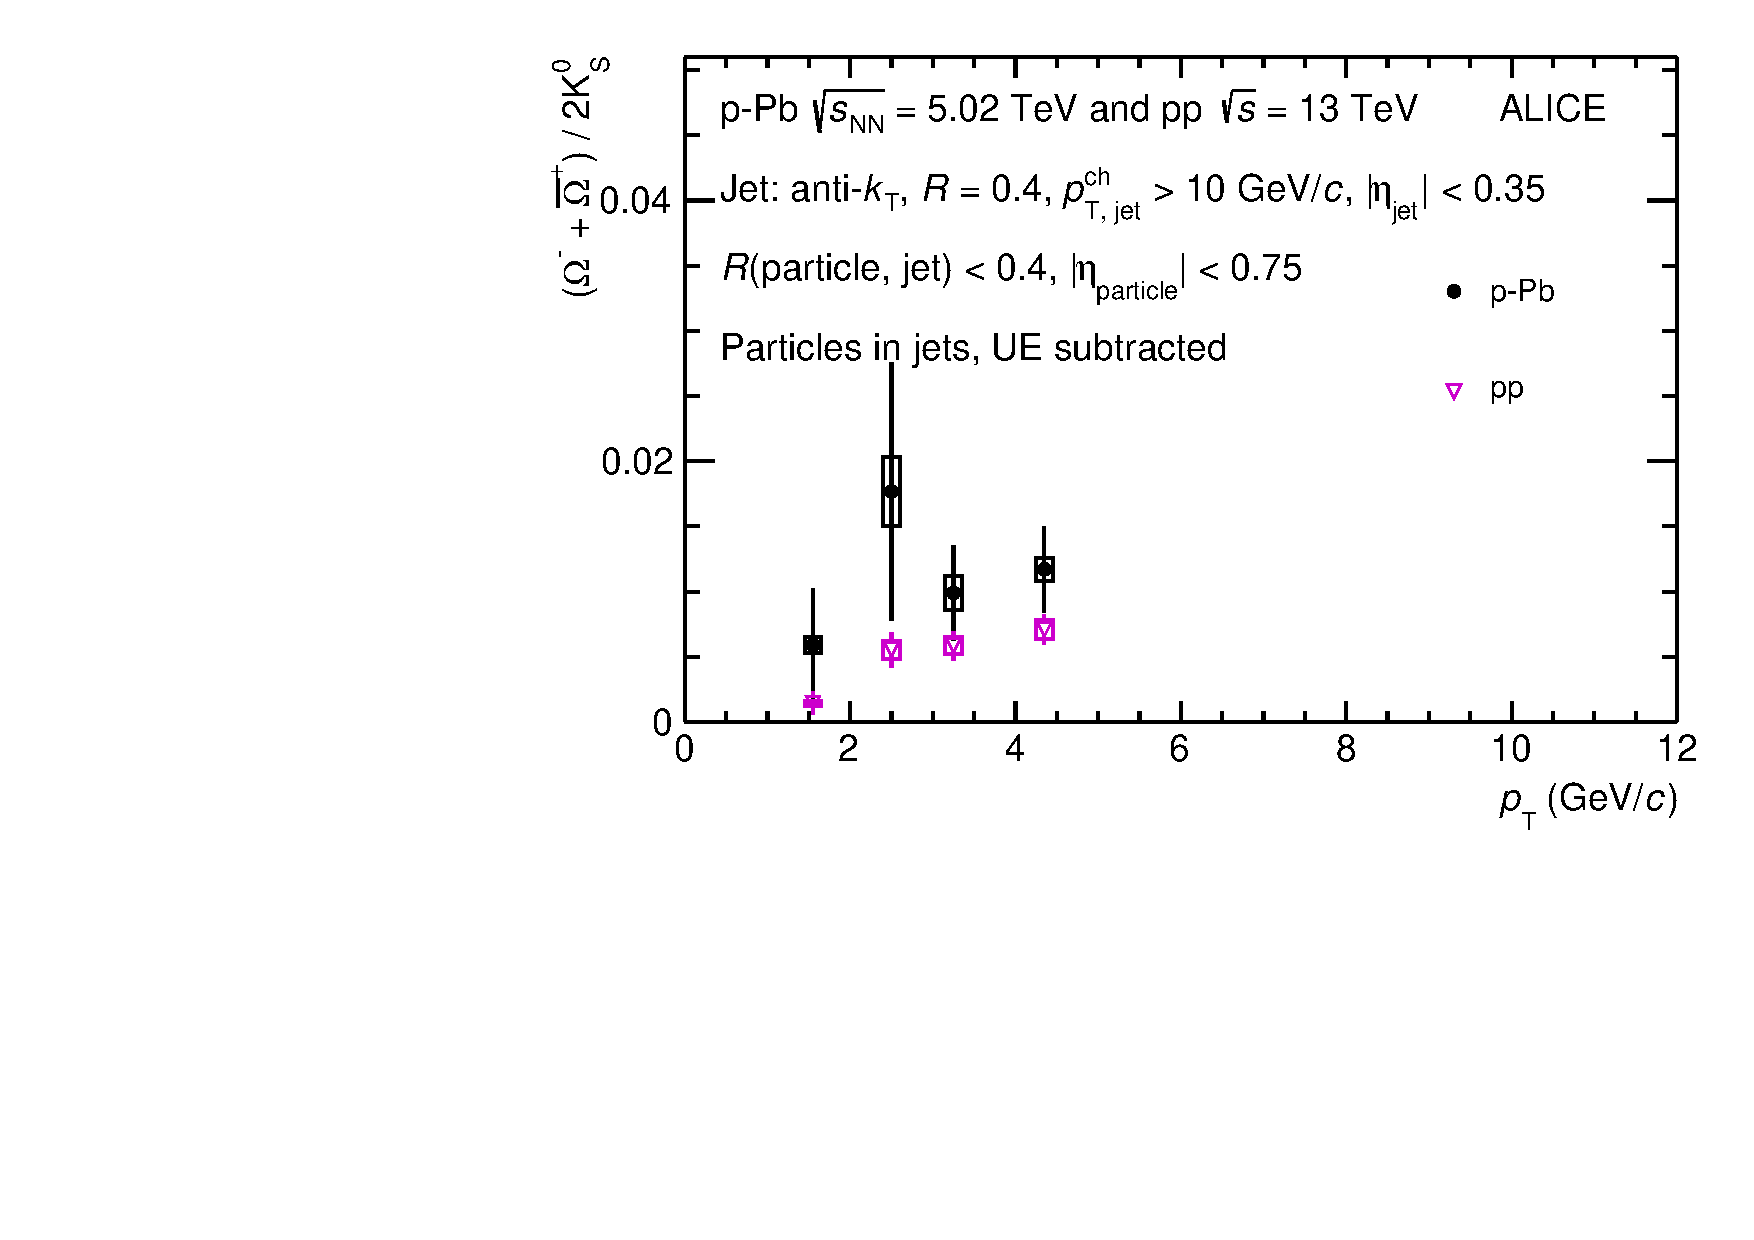
\includegraphics[width=.49\textwidth]{cf09_3}
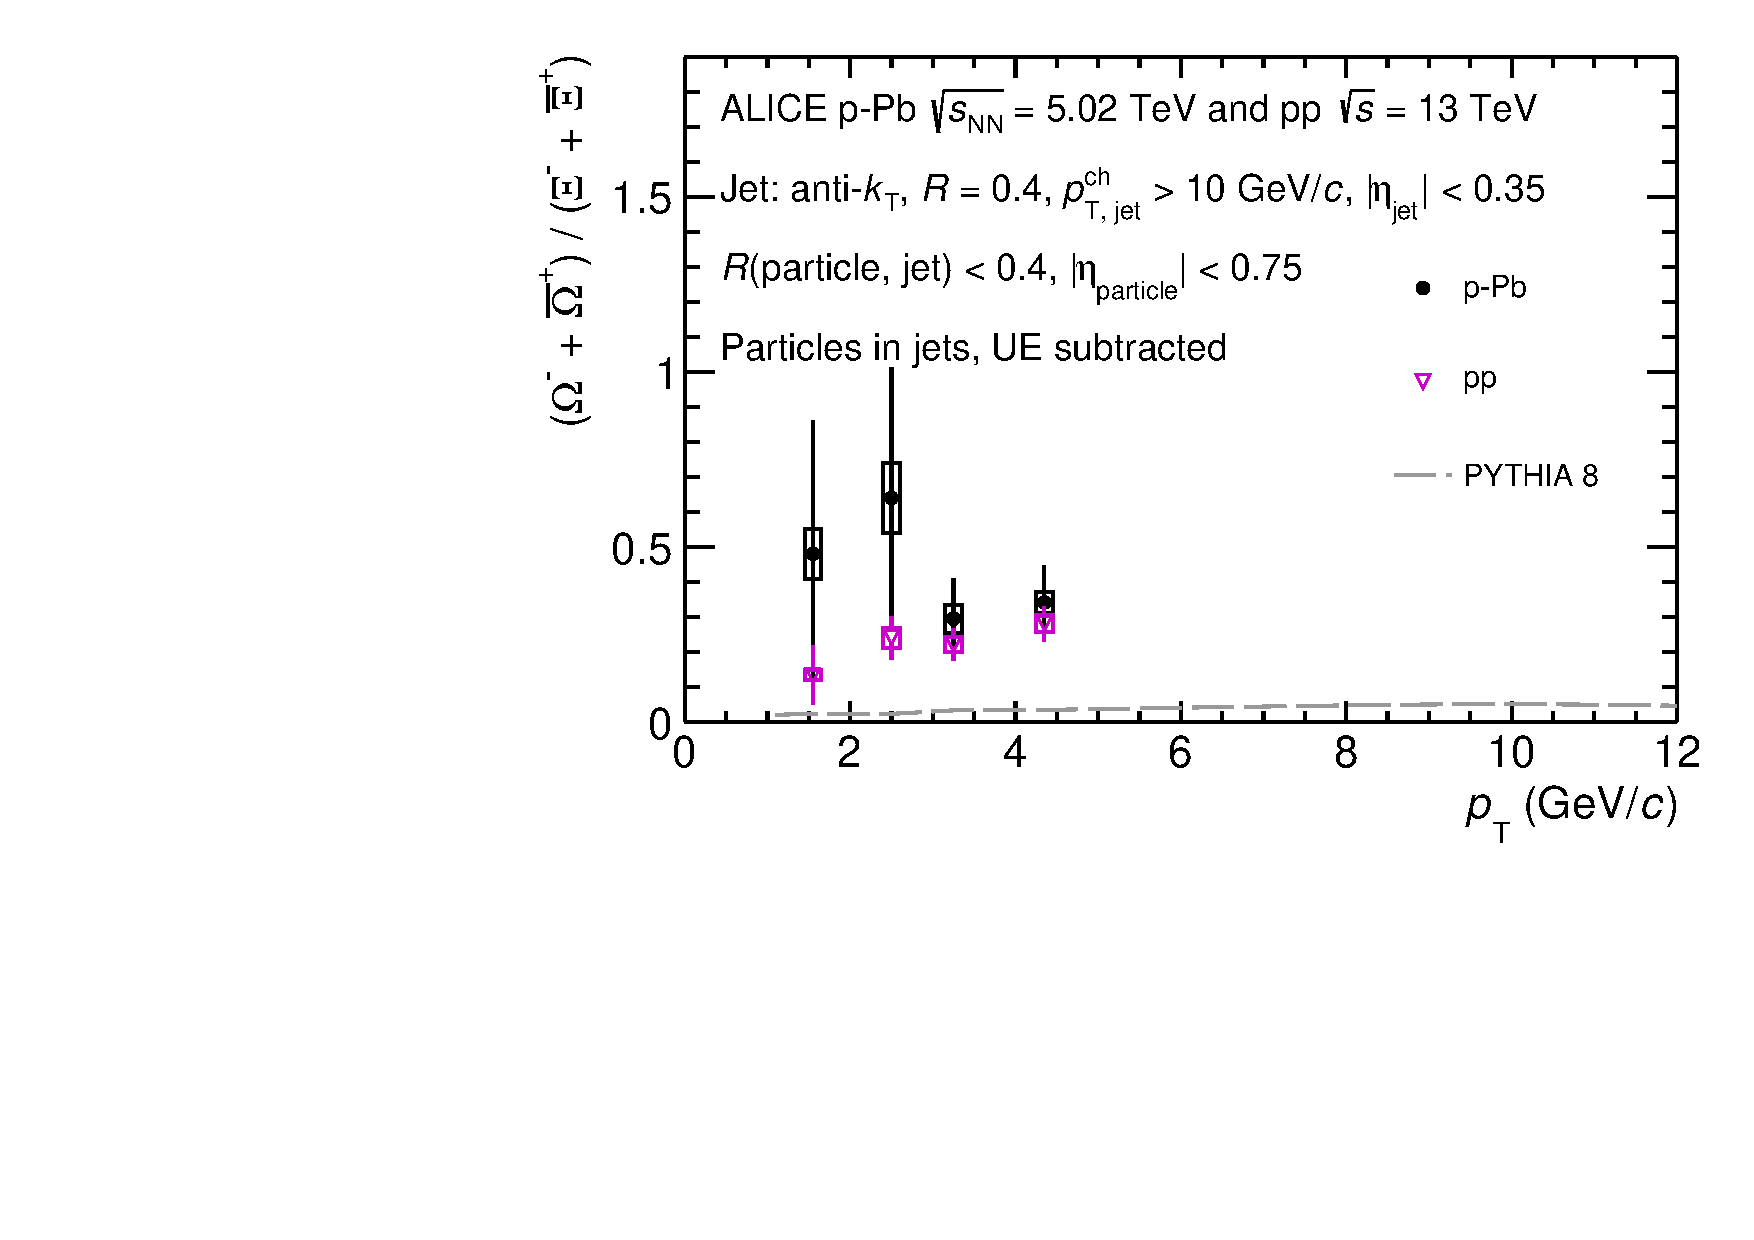
\includegraphics[width=.49\textwidth]{cf09_6}
\end{center}
\caption{The baryon-to-meson (left) and baryon-to-baryon (right) ratioin \pp (open symbols) collisions at \thirteen and \pPb (full symbols) collisions at \fivenn as a function of particle $\pT$ associated with charged particle jets with $\pTjch > 10$~\GeVc reconstructed using the \akT jet finder with resolution parameter $R = 0.4$. The ratios are shown for the same selection of the matching radius $R(\rm{particle, jet}) < 0.4$ in both systems. The different centrality classes for \pPb collisions are depicted with different color.The dashed curves represent PYTHIA 8 simulations to the measured ratios }
\label{fig:pppPbRatio}
\end{figure}

\clearpage
\section{Summary}%
\label{sec:Summary}

The first measurement of the \kzero, \lmb (\almb), \Xis and \Oms $\pT$-differential density, the $\lmb/\kzero$, $\Xi/\kzero$ and $\Omega/\kzero$ baryon-to-meson ratio and the $\Xi/\lmb$, $\Omega/\lmb$ and $\Omega/\Xi$ baryon-to-baryon ratio in charged-particle jets and underlying events in \pp collisions at \thirteen and \pPb collisions at \fivenn have been studied.
All the measured quantities are compared with PYTHIA 8 model predictions.
The PYTHIA 8 with the standard Monash trigg tune can describe the $\kzero, \lmb + \almb$, but not for the $\X + \Ix$ and $\Om + \Mo$.
The main aim of the presented analysis, based on charged-particle jet to separate hard and soft process, is to provide insight into the understanding of the origin of flow-like correlations observed in small systems.

For all particle the $\pT$-differential density in events with charged-particle jet ($\pTjch$ > 10~\GeVc) are observed to be harder than that in MB events.
In addition, the dependence on charged-particle multiplicity found in the inclusive particle is not present for particles generated by jet fragmentation.
The baryon-to-meson and baryon-to-baryon ratios associated with jets in \pPb collisions for $R({\rm particle, jet} < 0.4)$ is consistent with the ratio measured in \pp collisions.
The ratios are observed to be independent on the multiplicity class of \pPb collisions.
The enhancement of baryon-to-meson ratio at intermediate $\pT$ found in the inclusive particle are not present for particles associated with hard scattering tagged by jets reconstructed from charged particles for $\pTjch > 10$~\GeVc in \pp and \pPb collisions.
Moreover, as the baryon-to-meson enhancement has been linked to the interplay of radial flow and parton recombination at intermediate $\pT$, its absence within the jet cone demonstrates that these effects are indeed limited to the soft particle production process.

%%%%%%%%%%%%%%%%%%%%%%%%%%%%%%%%
% end main text
%%%%%%%%%%%%%%%%%%%%%%%%%%%%%%%%

%%%%% acknowledgements - handled by EB chairs
\newenvironment{acknowledgement}{\relax}{\relax}
\begin{acknowledgement}
\section*{Acknowledgements}
% add specific acknowledgements here
% ...but please don't remove the line below: funding agencies
% will be acknowledged with a custom tex file handled by EB chairs after Collab Round 2
%\input{acknowledgements.tex}
\end{acknowledgement}

%%%%%%%% Bibliography
\bibliographystyle{etc/utphys}
\bibliography{AliStrangeJets}

%%%%%%%%%%%%%%%%%%%%%%%%%%%%%%%%
% Appendices: yours (if any) + authorlist
%%%%%%%%%%%%%%%%%%%%%%%%%%%%%%%%
\newpage
\appendix
\section{Particle candidate selection criteria}
\begin{table}[!ht]
\begin{center}
\caption{\kzero(\lmb and \almb) candidate selection criteria of topological variables, daughter tracks and \Vzero candidates.
The DCA stands for the ``Distance of Closest Approach'', PV represents the ``Primary collision Vertex'' and CPA is the ``Cosine Pointing Angle between the momentum vector of the reconstructed \Vzero and the displacement vector between the decay and primary vertices''.}
\label{tab:V0Cut}
\begin{tabularx}{\textwidth}{@{} lCC @{}}
\toprule
\textbf{Topological variable} & \textbf{\pp} & \textbf{\pPb} \\
\midrule
$\Vzero$ transverse decay radius      & $> 0.5$~cm   & $> 0.5$~cm \\
DCA of positive / negative track to PV & $> 0.06$~cm  & $> 0.06$~cm \\
DCA between $\Vzero$ daughter tracks  & $< 1.0\sigma$ & $< 1\sigma$ \\
CPA of $\Vzero$ & $> 0.97$ ($0.995$) & $> 0.97$ ($0.995$) \\
\midrule
\textbf{Track selection} \\
\midrule
Daughter track pseudo-rapidity interval &$|\eta| < 0.8$ & $\abs{\eta} < 0.8$      \\
Daughter track $N_{\rm crossed~rows}$                   & $\geq 70$  & $\geq$ 70 \\
Daughter Track $N_{\rm crossed~rows}/N_{\rm findable}$  & $\geq 0.8$ & $\geq$ 0.8 \\
TPC $\dEdx$ & $< 5\sigma$ & $< 5\sigma$ \\
\midrule
\textbf{Candidate selection} \\
\midrule
Pseudo-rapidity interval & $|\eta| < 0.75$ & $|\eta| < 0.75$ \\
Proper lifetime($mL/p$)  & $< 20$ (30)~cm & $< 20$ (30)~cm \\
Competing mass & $> 0.005$ (0.010)~\GeVmass & $> 0.005$ (0.010)~\GeVmass \\
\bottomrule
\end{tabularx}
\end{center}
\end{table}

\begin{table}[!ht]
\begin{center}
\caption{\Xis(\Oms) candidate selection criteria of topological variables, daughter tracks and cascade candidates.}
\label{tab:CascadeCut}
\begin{tabularx}{\textwidth}{@{} lCC @{}}
\toprule
\textbf{Topological variable} & \textbf{\pp} & \textbf{\pPb} \\
\midrule
Cascade transverse decay radius & $> 0.8(0.6)$~cm & $> 0.6$~cm \\
\Vzero transverse decay radius & $> 1.4$~cm     & $> 1.2$~cm \\
DCA (bachelor to PV)           & $> 0.05$~cm    & $> 0.04$~cm \\
DCA (\Vzero to PV)             & $> 0.07$~cm    & $> 0.06$~cm \\
DCA (positive / negative track to PV) & $> 0.04(0.03)$~cm & $> 0.03$~cm  \\
DCA between \Vzero daughter tracks & $< 1.6\sigma$     & $< 1.5\sigma$ \\
DCA (bachelor to \Vzero) & $< 1.6(1.0)$~cm & $< 1.3$~cm \\
CPA of Cascade          & $> 0.97$       & $> 0.97$  \\
CPA of \Vzero           & $> 0.97$       & $> 0.97$  \\
\Vzero invariant mass window & $\pm 0.006$~\GeVmass & $\pm 0.008$~\GeVmass \\
\midrule
\textbf{Track selection} \\
\midrule
Daughter track pseudo-rapidity interval & $|\eta| < 0.8$ & $|\eta| < 0.8$ \\
Daughter track $N_{\rm crossed~rows}$  & $\geq 70$      & $\geq$ 70 \\
Daughter Track $N_{\rm crossed~rows}/N_{\rm findable}$ &$\geq 0.8$ &$\geq$ 0.8 \\
TPC $\dEdx$ & $< 5\sigma$ & $< 4\sigma$ \\
\midrule
\textbf{Candidate selection} \\
\midrule
Pseudo-rapidity interval & $|\eta| < 0.75$ &$|\eta| < 0.75$ \\
Proper lifetime ($mL/p$) & & $< 3 \times c\tau$ \\
Competing mass          & $8$~\MeVmass & $8$~\MeVmass \\
\bottomrule
\end{tabularx}
\end{center}
\end{table}

%%%%% Authorlist - please do not touch: handled by EB chairs
\section{The ALICE Collaboration}
\label{app:collab}
%\input{authorlist-preprint.tex}
\end{document}